\setlength{\parindent}{0pt}
\chapter{\bf APPENDIX} 

\shorthandoff{=}

\begin{figure}[H]
\begin{center}
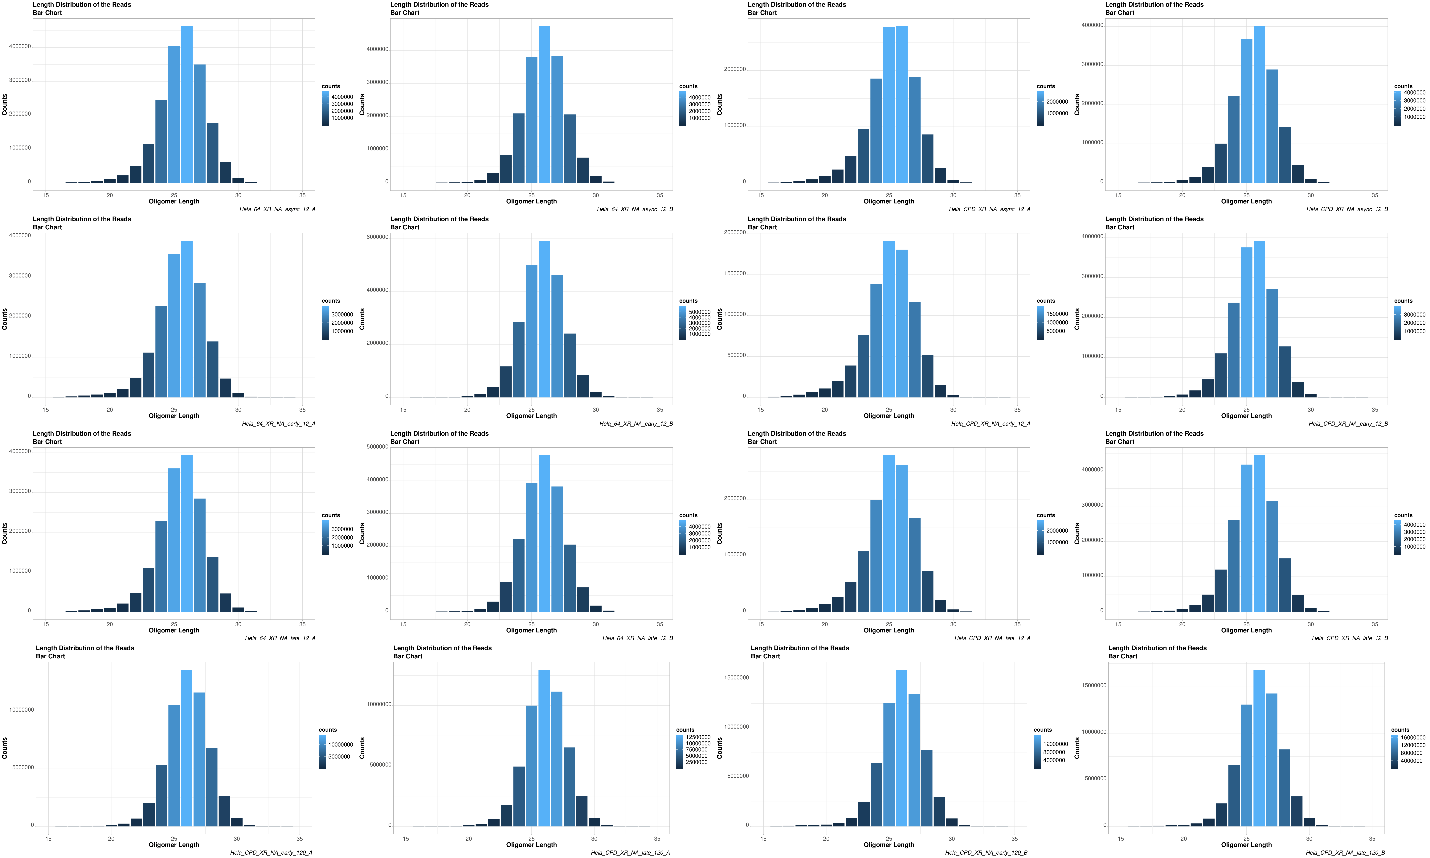
\includegraphics[width=\textwidth]{Chapters/7_appendix/figures/supfig1}
\caption[Length distribution of excised oligomers of XR-seq samples.]{Length distribution of excised oligomers of XR-seq samples after adaptor trimming and duplicate removal. Majority of the oligomers are 26 nucleotides long.}
\label{supfig:length}
\end{center}
\end{figure}


\begin{figure}[H]
\begin{center}
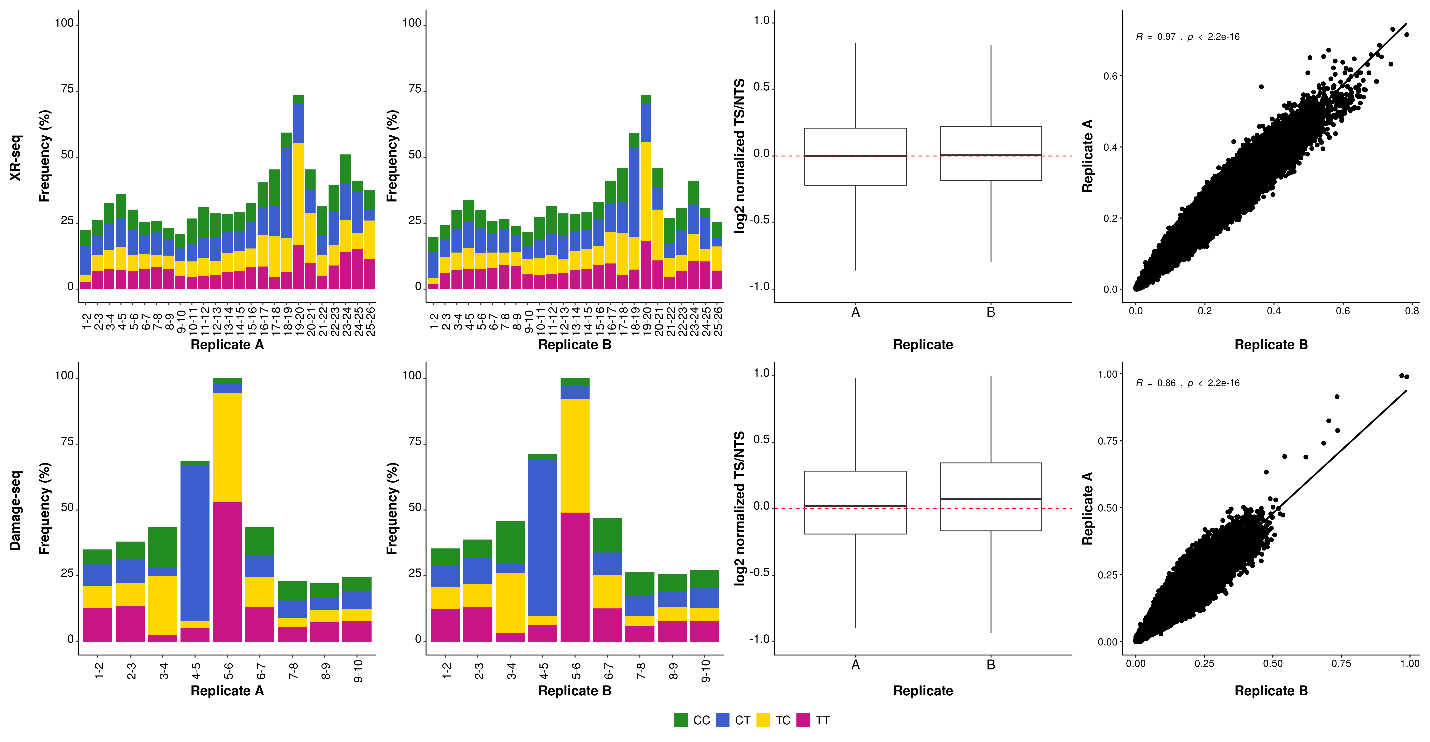
\includegraphics[width=\textwidth]{Chapters/7_appendix/figures/supfig2}
\caption[Control figures of (6-4)PP asynchronized samples at 12 minutes.]{Control figures of (6-4)PP asynchronized samples at 12 minutes. Column 1 is the correlation plot of the biological replicates (A \& B). Column 1 and 2 displays the dinucleotide composition frequency of replicate A and B, respectively. Column 3 is the log2 transformed TS/NTS ratios of replicate A and B. Row 1 is the results of XR-seq samples, and row 2 is the results of Damage-seq samples. Column 4 is the correlation plot of the biological replicates (A \& B). Correlation coefficient is calculated by Spearman’s rank correlation test.}
\label{supfig:control1}
\end{center}
\end{figure}


\begin{figure}[H]
\begin{center}
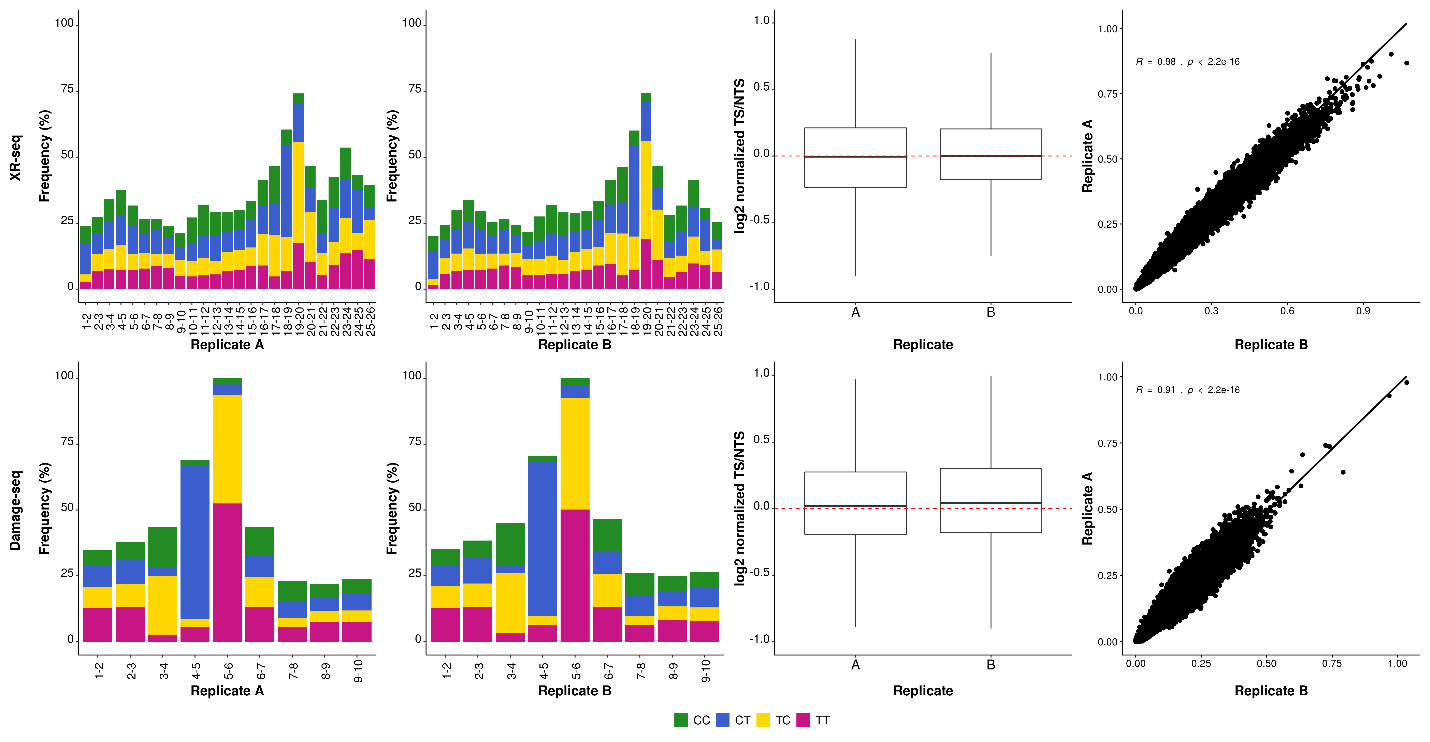
\includegraphics[width=\textwidth]{Chapters/7_appendix/figures/supfig3}
\caption[Control figures of (6-4)PP early phased samples at 12 minutes.]{Control figures of (6-4)PP early phased samples at 12 minutes. Column 1 is the correlation plot of the biological replicates (A \& B). Column 1 and 2 displays the dinucleotide composition frequency of replicate A and B, respectively. Column 3 is the log2 transformed TS/NTS ratios of replicate A and B. Row 1 is the results of XR-seq samples, and row 2 is the results of Damage-seq samples. Column 4 is the correlation plot of the biological replicates (A \& B). Correlation coefficient is calculated by Spearman’s rank correlation test.}
\label{supfig:control2}
\end{center}
\end{figure}


\begin{figure}[H]
\begin{center}
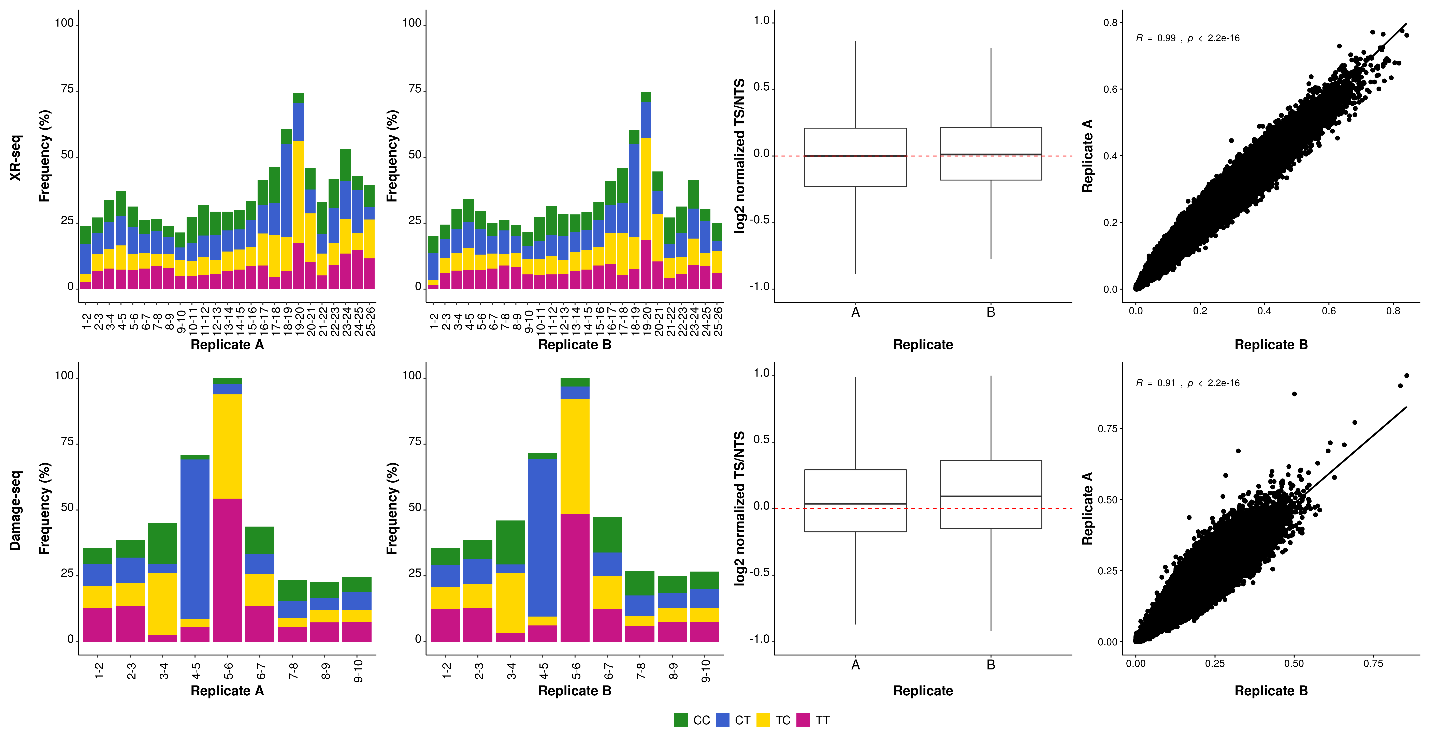
\includegraphics[width=\textwidth]{Chapters/7_appendix/figures/supfig4}
\caption[Control figures of (6-4)PP late phased samples at 12 minutes.]{Column 1 is the correlation plot of the biological replicates (A \& B). Column 1 and 2 displays the dinucleotide composition frequency of replicate A and B, respectively. Column 3 is the log2 transformed TS/NTS ratios of replicate A and B. Row 1 is the results of XR-seq samples, and row 2 is the results of Damage-seq samples. Column 4 is the correlation plot of the biological replicates (A \& B). Correlation coefficient is calculated by Spearman’s rank correlation test.}
\label{supfig:control3}
\end{center}
\end{figure}


\begin{figure}[H]
\begin{center}
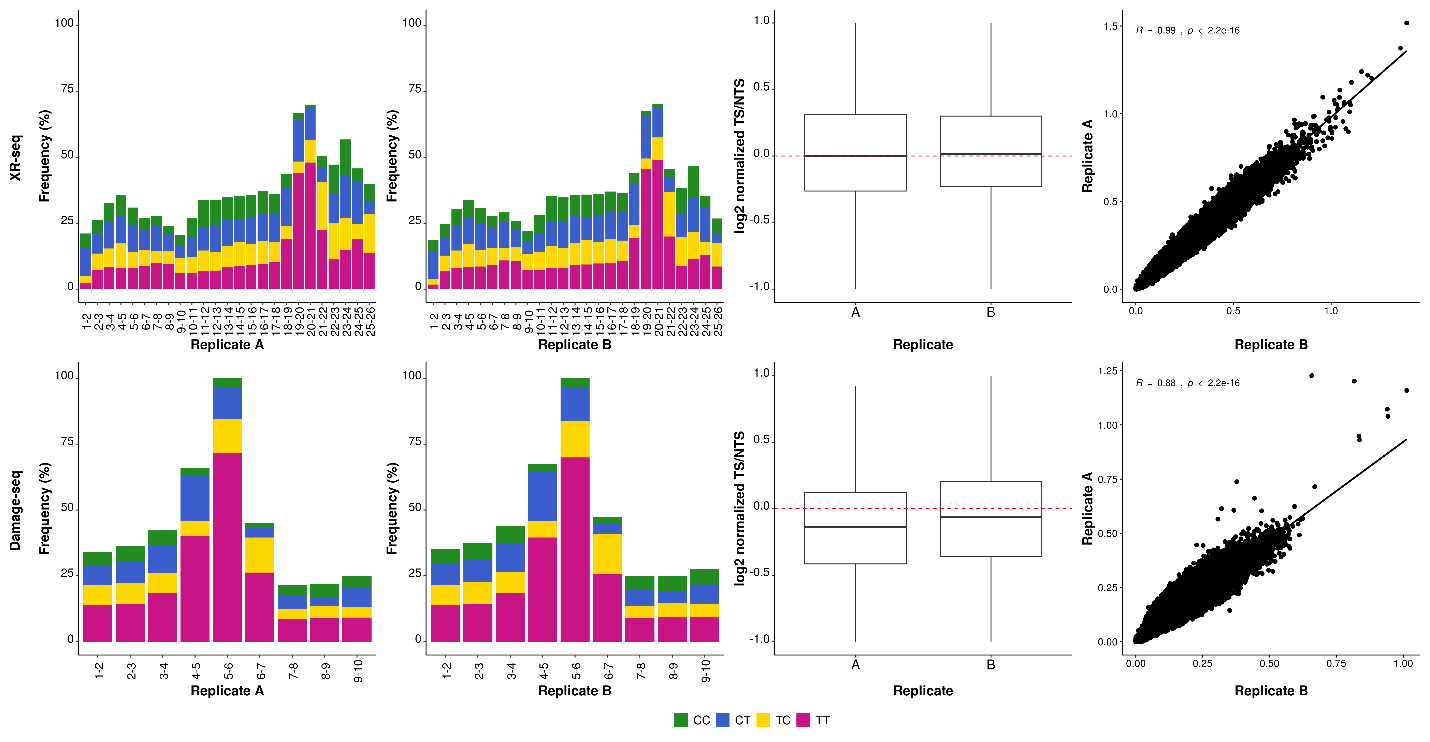
\includegraphics[width=\textwidth]{Chapters/7_appendix/figures/supfig5}
\caption[Control figures of CPD asynchronized samples at 12 minutes.]{Control figures of CPD asynchronized samples at 12 minutes. Column 1 is the correlation plot of the biological replicates (A \& B). Column 1 and 2 displays the dinucleotide composition frequency of replicate A and B, respectively. Column 3 is the log2 transformed TS/NTS ratios of replicate A and B. Row 1 is the results of XR-seq samples, and row 2 is the results of Damage-seq samples. Column 4 is the correlation plot of the biological replicates (A \& B). Correlation coefficient is calculated by Spearman’s rank correlation test.}
\label{supfig:control4}
\end{center}
\end{figure}


\begin{figure}[H]
\begin{center}
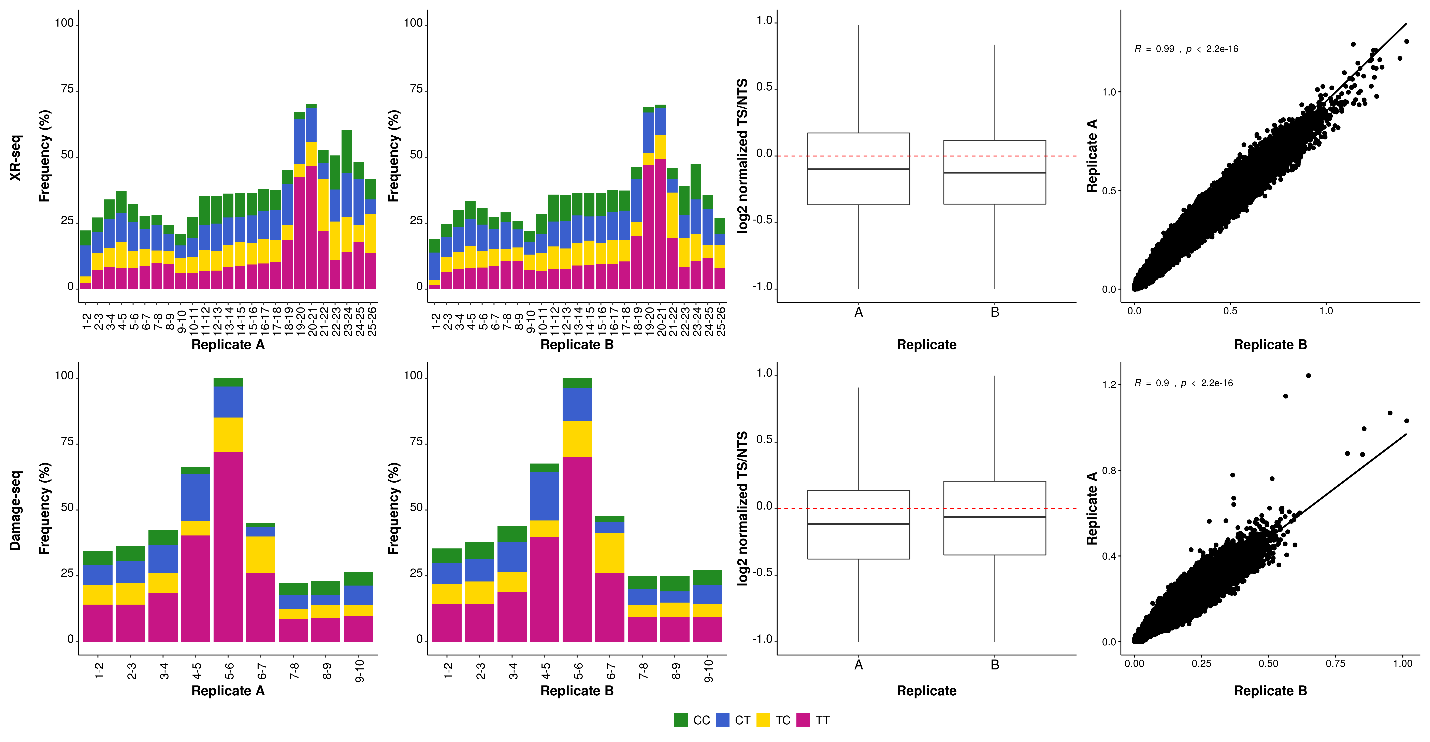
\includegraphics[width=\textwidth]{Chapters/7_appendix/figures/supfig6}
\caption[Control figures of CPD early phased samples at 12 minutes.]{Control figures of CPD early phased samples at 12 minutes. Column 1 is the correlation plot of the biological replicates (A \& B). Column 1 and 2 displays the dinucleotide composition frequency of replicate A and B, respectively. Column 3 is the log2 transformed TS/NTS ratios of replicate A and B. Row 1 is the results of XR-seq samples, and row 2 is the results of Damage-seq samples. Column 4 is the correlation plot of the biological replicates (A \& B). Correlation coefficient is calculated by Spearman’s rank correlation test.}
\label{supfig:control5}
\end{center}
\end{figure}


\begin{figure}[H]
    \begin{center}
    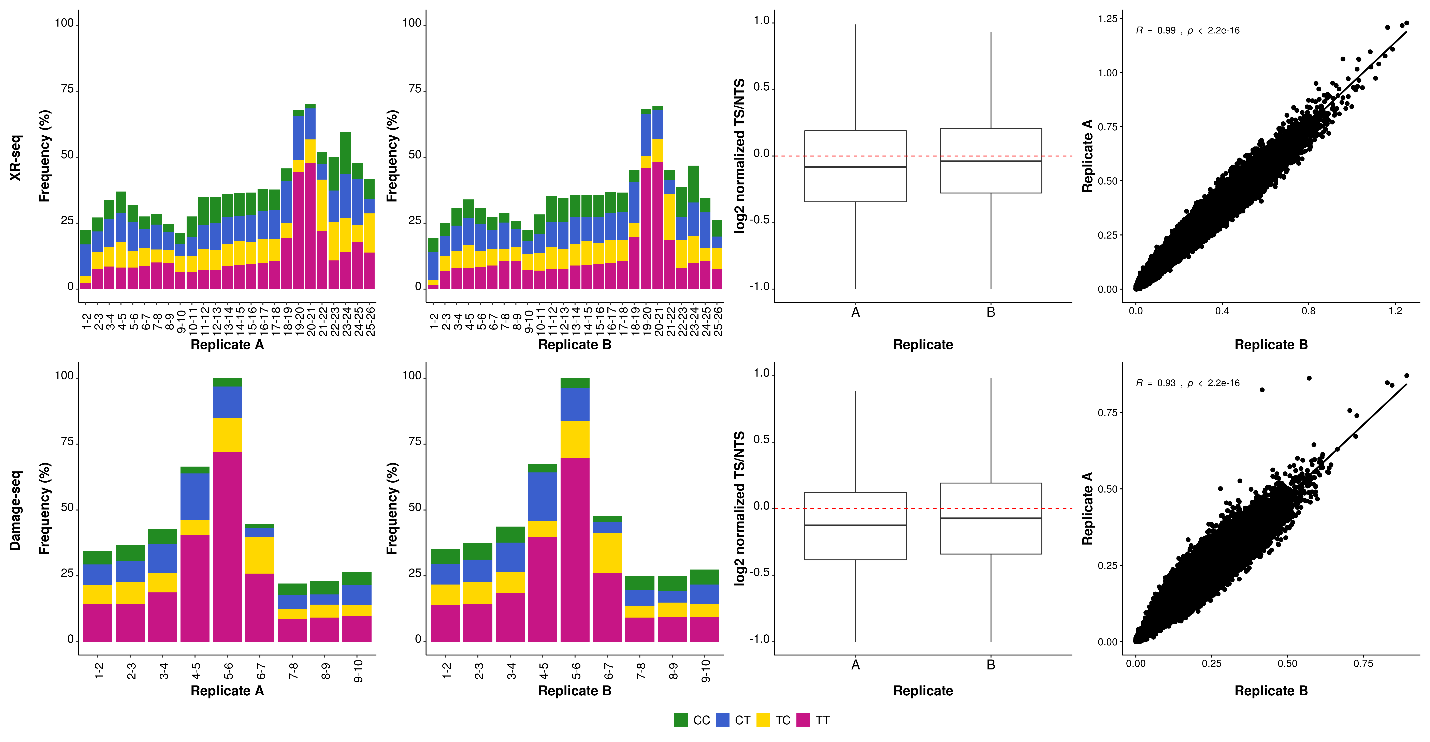
\includegraphics[width=\textwidth]{Chapters/7_appendix/figures/supfig7}
    \caption[Control figures of CPD late phased samples at 12 minutes.]{Control figures of CPD late phased samples at 12 minutes. Column 1 is the correlation plot of the biological replicates (A \& B). Column 1 and 2 displays the dinucleotide composition frequency of replicate A and B, respectively. Column 3 is the log2 transformed TS/NTS ratios of replicate A and B. Row 1 is the results of XR-seq samples, and row 2 is the results of Damage-seq samples. Column 4 is the correlation plot of the biological replicates (A \& B). Correlation coefficient is calculated by Spearman’s rank correlation test.}
    \label{supfig:control6}
    \end{center}
    \end{figure}

\begin{figure}[H]
    \begin{center}
    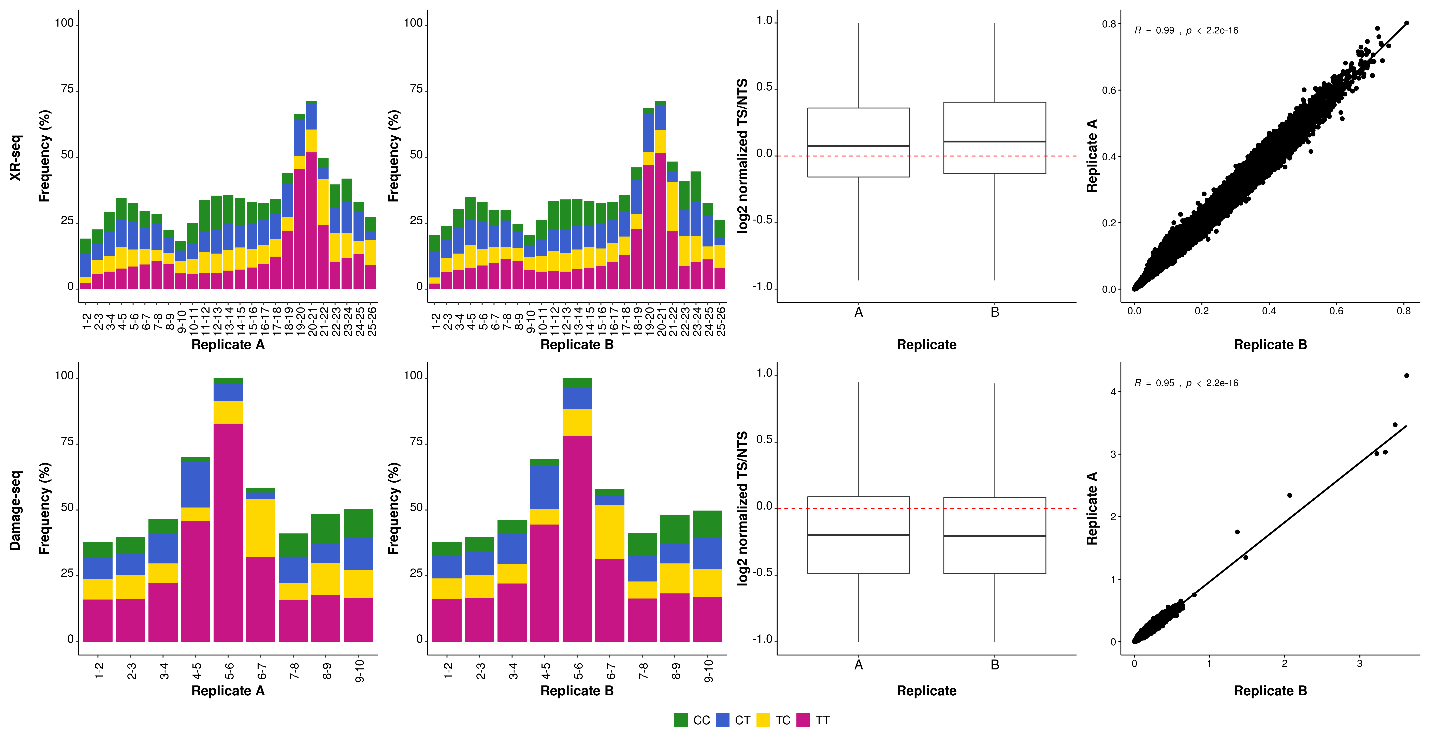
\includegraphics[width=\textwidth]{Chapters/7_appendix/figures/supfig8}
    \caption[Control figures of CPD early phased samples at 120 minutes.]{Control figures of CPD early phased samples at 120 minutes. Column 1 is the correlation plot of the biological replicates (A \& B). Column 1 and 2 displays the dinucleotide composition frequency of replicate A and B, respectively. Column 3 is the log2 transformed TS/NTS ratios of replicate A and B. Row 1 is the results of XR-seq samples, and row 2 is the results of Damage-seq samples. Column 4 is the correlation plot of the biological replicates (A \& B). Correlation coefficient is calculated by Spearman’s rank correlation test.}
    \label{supfig:control7}
    \end{center}
    \end{figure}

\begin{figure}[H]
    \begin{center}
    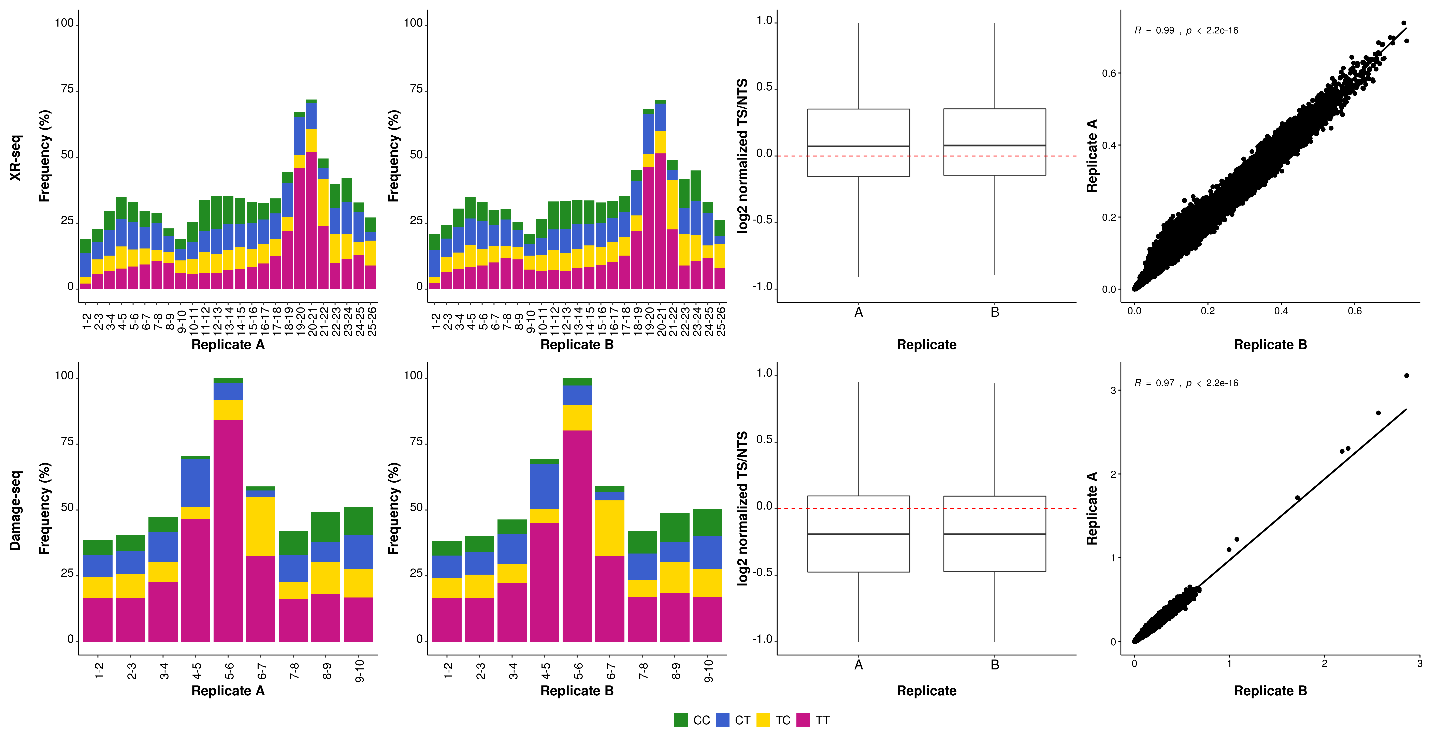
\includegraphics[width=\textwidth]{Chapters/7_appendix/figures/supfig9}
    \caption[Control figures of CPD late phased samples at 120 minutes.]{Control figures of CPD late phased samples at 120 minutes. Column 1 is the correlation plot of the biological replicates (A \& B). Column 1 and 2 displays the dinucleotide composition frequency of replicate A and B, respectively. Column 3 is the log2 transformed TS/NTS ratios of replicate A and B. Row 1 is the results of XR-seq samples, and row 2 is the results of Damage-seq samples. Column 4 is the correlation plot of the biological replicates (A \& B). Correlation coefficient is calculated by Spearman’s rank correlation test.}
    \label{supfig:control8}
    \end{center}
    \end{figure}

\begin{figure}[H]
\begin{center}
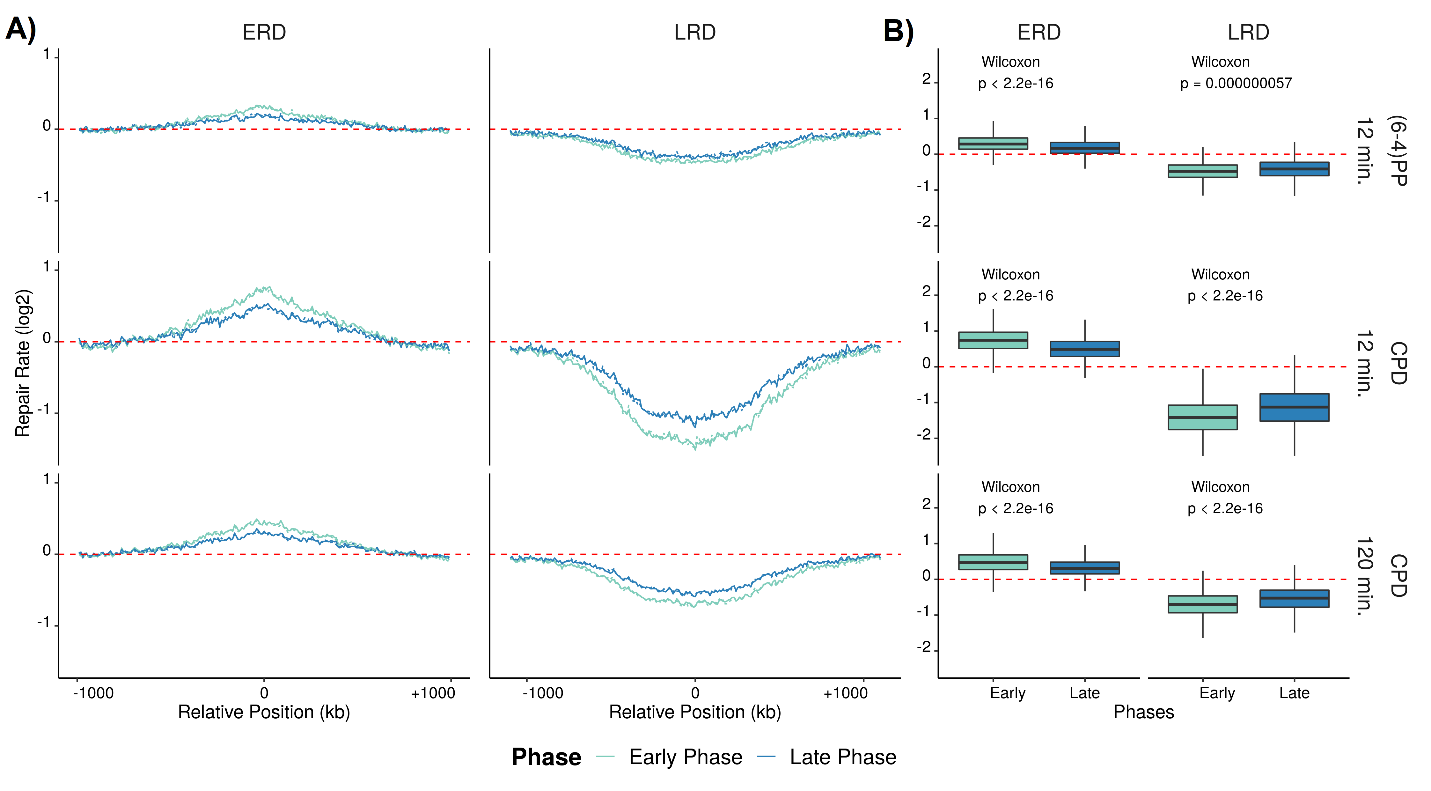
\includegraphics[width=\textwidth]{Chapters/7_appendix/figures/supfig10}
\caption[The shift of repair efficiency at replication domains during replication.]{The shift of repair efficiency at replication domains during replication. A) Repair rates (XR-seq/Damage-seq) are calculated and log2 transformed in 2 Mbp regions with 10 kb intervals, which early replication domains (ERDs, left) and late replication domains (LRDs, right) positioned at the center of the region. B) RPKM values of XR-seq samples are divided by Damage-seq samples (Repair Rate) for both ERDs (left) and LRDs (right) and log2 transformed. Wilcoxon test is used to assess the significance of difference between early and late S phases. The light blue lines are the early phase repair rate values and dark blue lines are the late phase repair rate values. Above the red horizontal dashed line demonstrates that repair is higher than damage, below demonstrates that damage is higher. (Same analysis as Figure 2, it is performed with replicate B)}
\label{supfig:repdomain}
\end{center}
\end{figure}

\begin{figure}[H]
\begin{center}
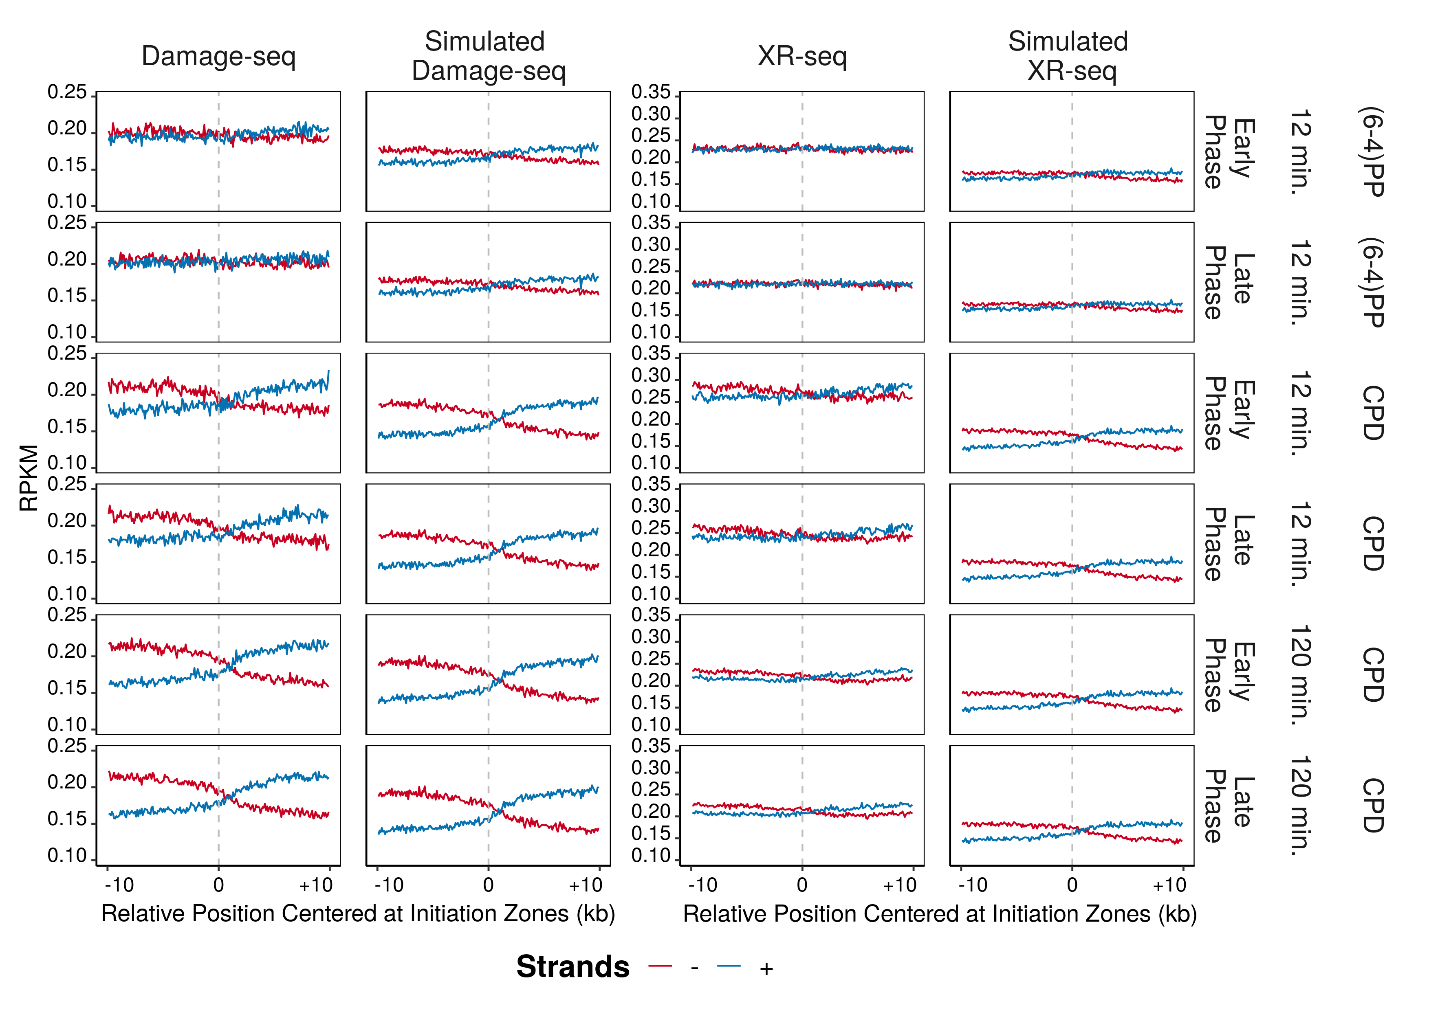
\includegraphics[width=\textwidth]{Chapters/7_appendix/figures/supfig11}
\caption[Strand asymmetry around initiation zones caused by nucleotide bias.]{Strand asymmetry around initiation zones caused by nucleotide bias. RPKM values of real and simulated Damage-seq samples (left) and XR-seq samples (right) are calculated in 20 kb windows with 100 base pair intervals, which Initiation Zones are positioned at the center of the region. Blue lines represent the plus strands and red lines represent the minus strands. Gray vertical dashed line shows the center of the region. (Same analysis as Figure 4, it is performed with replicate B)}
\label{supfig:simulation}
\end{center}
\end{figure}

\begin{figure}[H]
\begin{center}
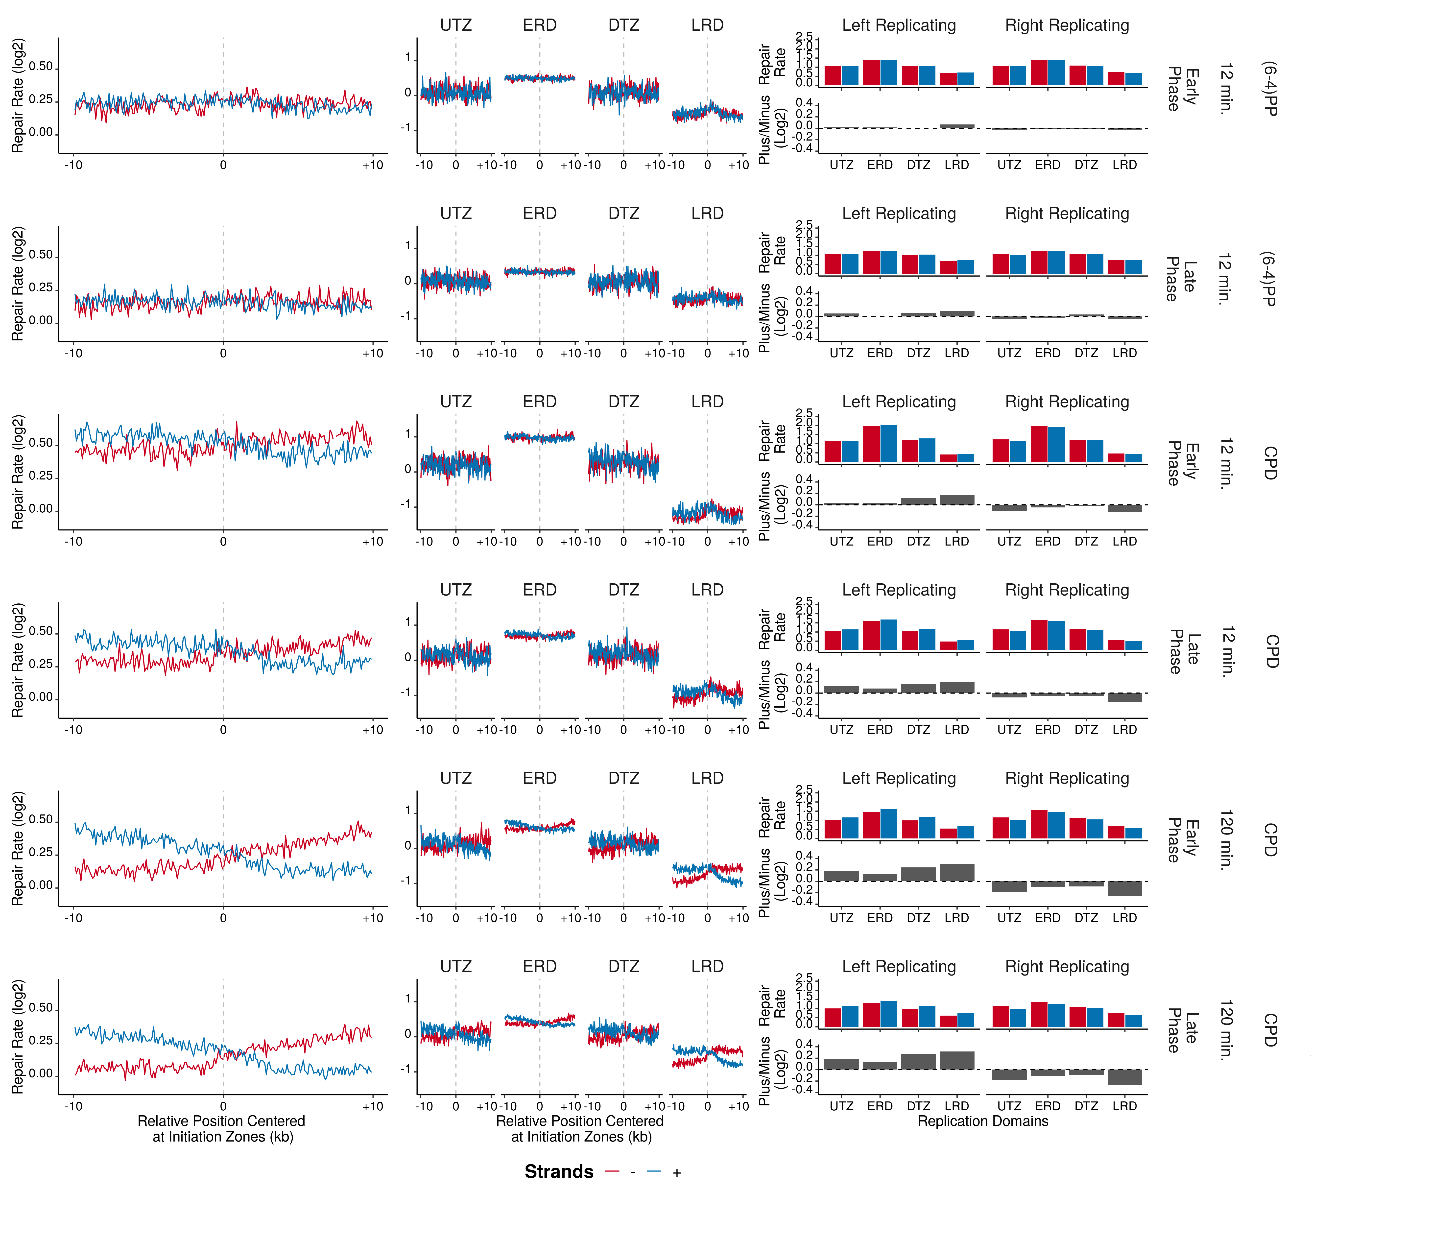
\includegraphics[width=\textwidth]{Chapters/7_appendix/figures/supfig12}
\caption[Repair rate asymmetry around initiation zones and replication domains.]{Repair rate asymmetry around initiation zones and replication domains. (Left) Repair rates (XR-seq/Damage-seq) are calculated and log2 transformed in 20 kb windows with 100 base pair intervals, which Initiation Zones are positioned at the center of the region. (Middle) Same analysis performed, however initiation zones separated into their corresponding replication domains. (Right) The strand differences at left (left part of the gray line) and right (right part of the gray line) replicating directions are shown by taking the mean of the intervals, separately for the strands. Below that, strands are divided to each other (Plus/Minus) and log2 transformed to better visualize the asymmetry at each replication domain. Blue lines are the plus strands and red lines are the minus strands. Gray vertical dashed line shows the center of the region. (Same analysis as Figure 6, it is performed with replicate B)}
\label{supfig:repairrate}
\end{center}
\end{figure}

\begin{figure}[H]
\begin{center}
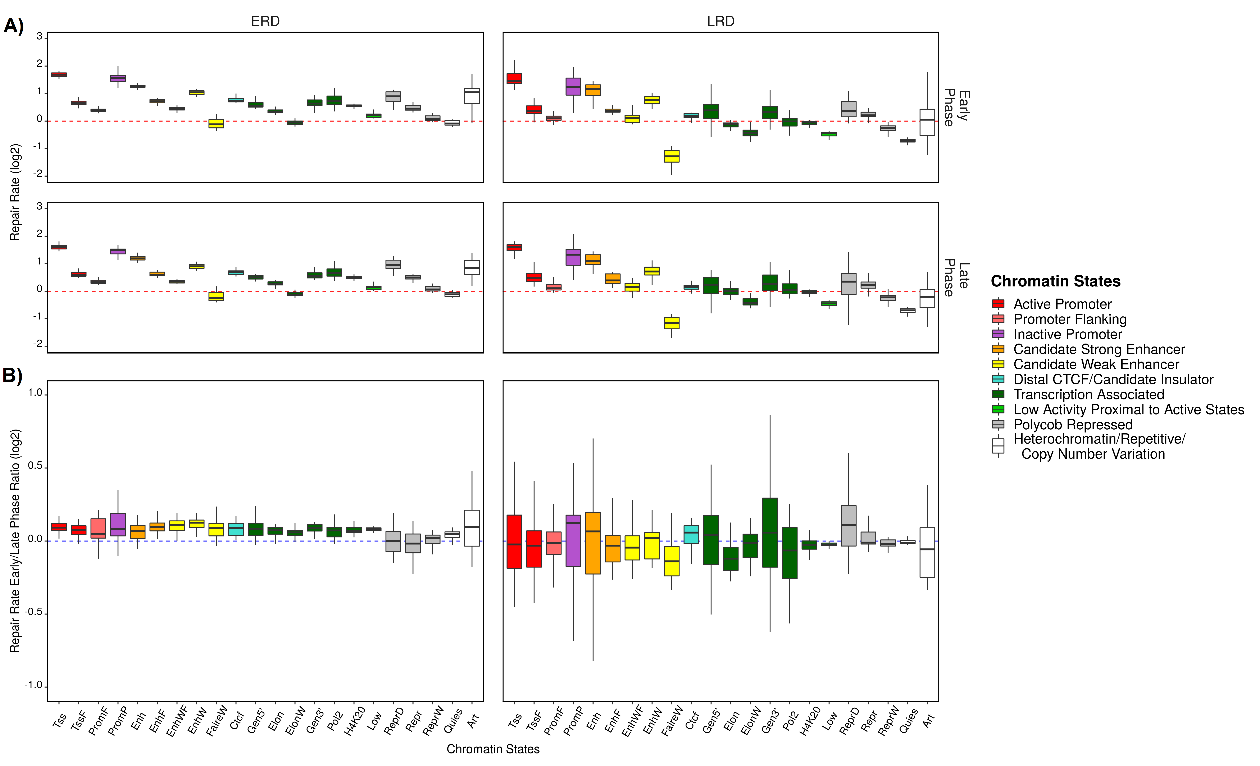
\includegraphics[width=\textwidth]{Chapters/7_appendix/figures/supfig13}
\caption[The effect of Chromatin States to repair efficiency of replication domains for (6-4)PP samples at 12 minutes (replicate A).]{The effect of Chromatin States to repair efficiency of replication domains. A) Repair rates (XR-seq/Damage-seq) of (6-4)PP samples at 12 minutes are calculated, log2 transformed B) and for every region, the repair rates at early S phase divided by repair rates at late S phase to spot the chromatin states that are repaired dominant at a phase. Above the red horizontal dashed line demonstrates that repair is higher than damage (A), and the blue horizontal dashed line demonstrates that the chromatin state has higher repair efficiency at early S phase than it has at late S phase (B). Analysis is performed on replicate A.}
\label{supfig:chromatin1}
\end{center}
\end{figure}

\begin{figure}[H]
\begin{center}
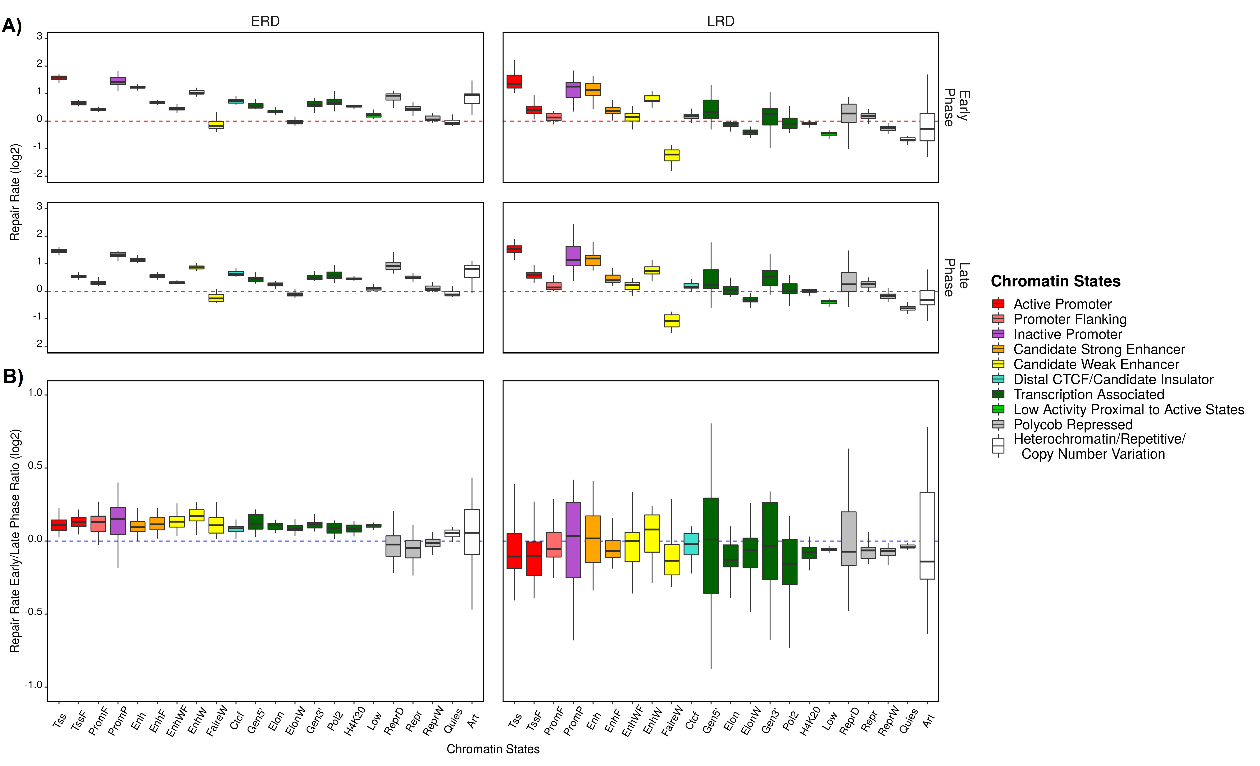
\includegraphics[width=\textwidth]{Chapters/7_appendix/figures/supfig14}
\caption[The effect of Chromatin States to repair efficiency of replication domains for (6-4)PP samples at 12 minutes (replicate A).]{The effect of Chromatin States to repair efficiency of replication domains. A) Repair rates (XR-seq/Damage-seq) of (6-4)PP samples at 12 minutes are calculated, log2 transformed, B) and for every region, the repair rates at early S phase divided by repair rates at late S phase to spot the chromatin states that are repaired dominant at a phase. Above the red horizontal dashed line demonstrates that repair is higher than damage (A), and the blue horizontal dashed line demonstrates that the chromatin state has higher repair efficiency at early S phase than it has at late S phase (B). Analysis is performed on replicate B.}
\label{supfig:chromatin2}
\end{center}
\end{figure}

\begin{figure}[H]
\begin{center}
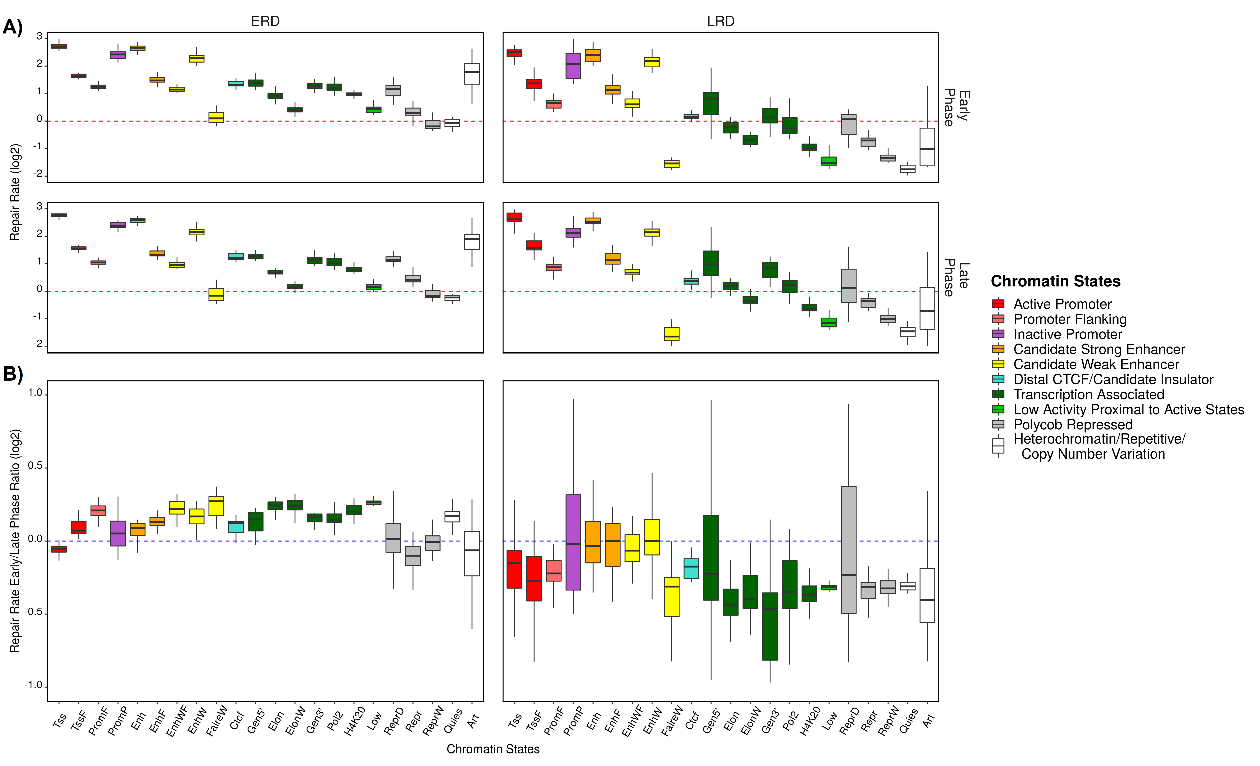
\includegraphics[width=\textwidth]{Chapters/7_appendix/figures/supfig15}
\caption[The effect of Chromatin States to repair efficiency of replication domains for CPD samples at 12 minutes (replicate B).]{The effect of Chromatin States to repair efficiency of replication domains. A) Repair rates (XR-seq/Damage-seq) of CPD samples at 12 minutes are calculated, log2 transformed, B) and for every region, the repair rates at early S phase divided by repair rates at late S phase to spot the chromatin states that are repaired dominant at a phase. Above the red horizontal dashed line demonstrates that repair is higher than damage (A), and the blue horizontal dashed line demonstrates that the chromatin state has higher repair efficiency at early S phase than it has at late S phase (B). (Same analysis as Figure 3, it is performed with replicate B)}
\label{supfig:chromatin3}
\end{center}
\end{figure}

\begin{figure}[H]
\begin{center}
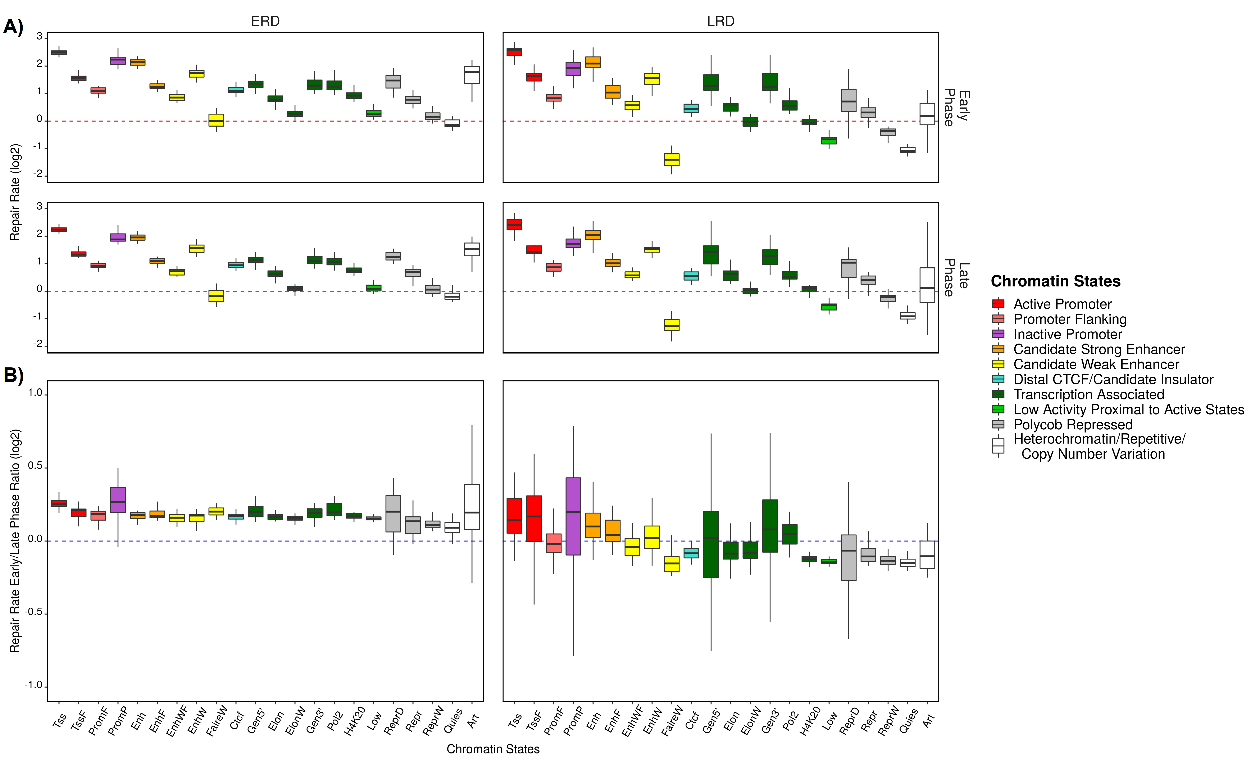
\includegraphics[width=\textwidth]{Chapters/7_appendix/figures/supfig16}
\caption[The effect of Chromatin States to repair efficiency of replication domains for CPD samples at 120 minutes (replicate A).]{The effect of Chromatin States to repair efficiency of replication domains. A) Repair rates (XR-seq/Damage-seq) of CPD samples at 120 minutes are calculated, log2 transformed, B) and for every region, the repair rates at early S phase divided by repair rates at late S phase to spot the chromatin states that are repaired dominant at a phase. Above the red horizontal dashed line demonstrates that repair is higher than damage (A), and the blue horizontal dashed line demonstrates that the chromatin state has higher repair efficiency at early S phase than it has at late S phase (B). Analysis is performed on replicate A.}
\label{supfig:chromatin4}
\end{center}
\end{figure}

\begin{figure}[H]
\begin{center}
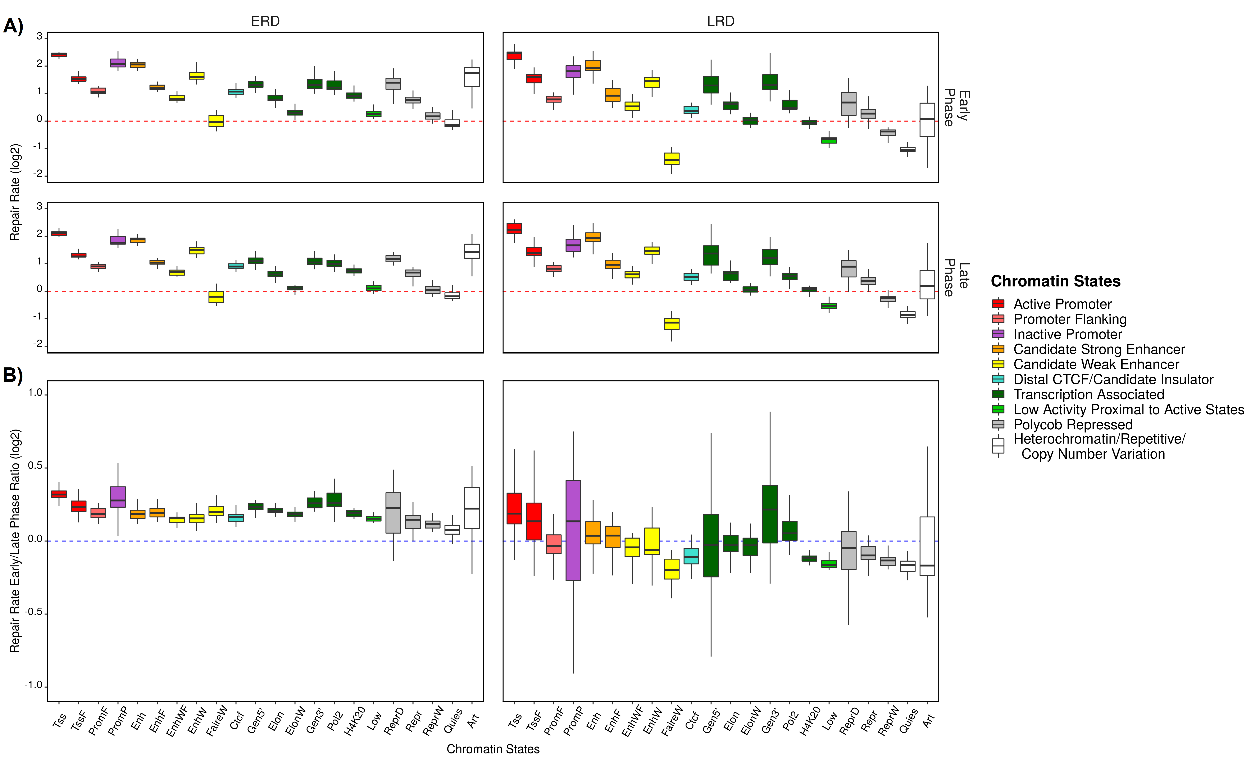
\includegraphics[width=\textwidth]{Chapters/7_appendix/figures/supfig17}
\caption[The effect of Chromatin States to repair efficiency of replication domains for CPD samples at 120 minutes (replicate B).]{The effect of Chromatin States to repair efficiency of replication domains. A) Repair rates (XR-seq/Damage-seq) of CPD samples at 120 minutes are calculated, log2 transformed B) and for every region, the repair rates at early S phase divided by repair rates at late S phase to spot the chromatin states that are repaired dominant at a phase. Above the red horizontal dashed line demonstrates that repair is higher than damage (A), and the blue horizontal dashed line demonstrates that the chromatin state has higher repair efficiency at early S phase than it has at late S phase (B). Analysis is performed on replicate B.}
\label{supfig:chromatin5}
\end{center}
\end{figure}

\begin{figure}[H]
\begin{center}
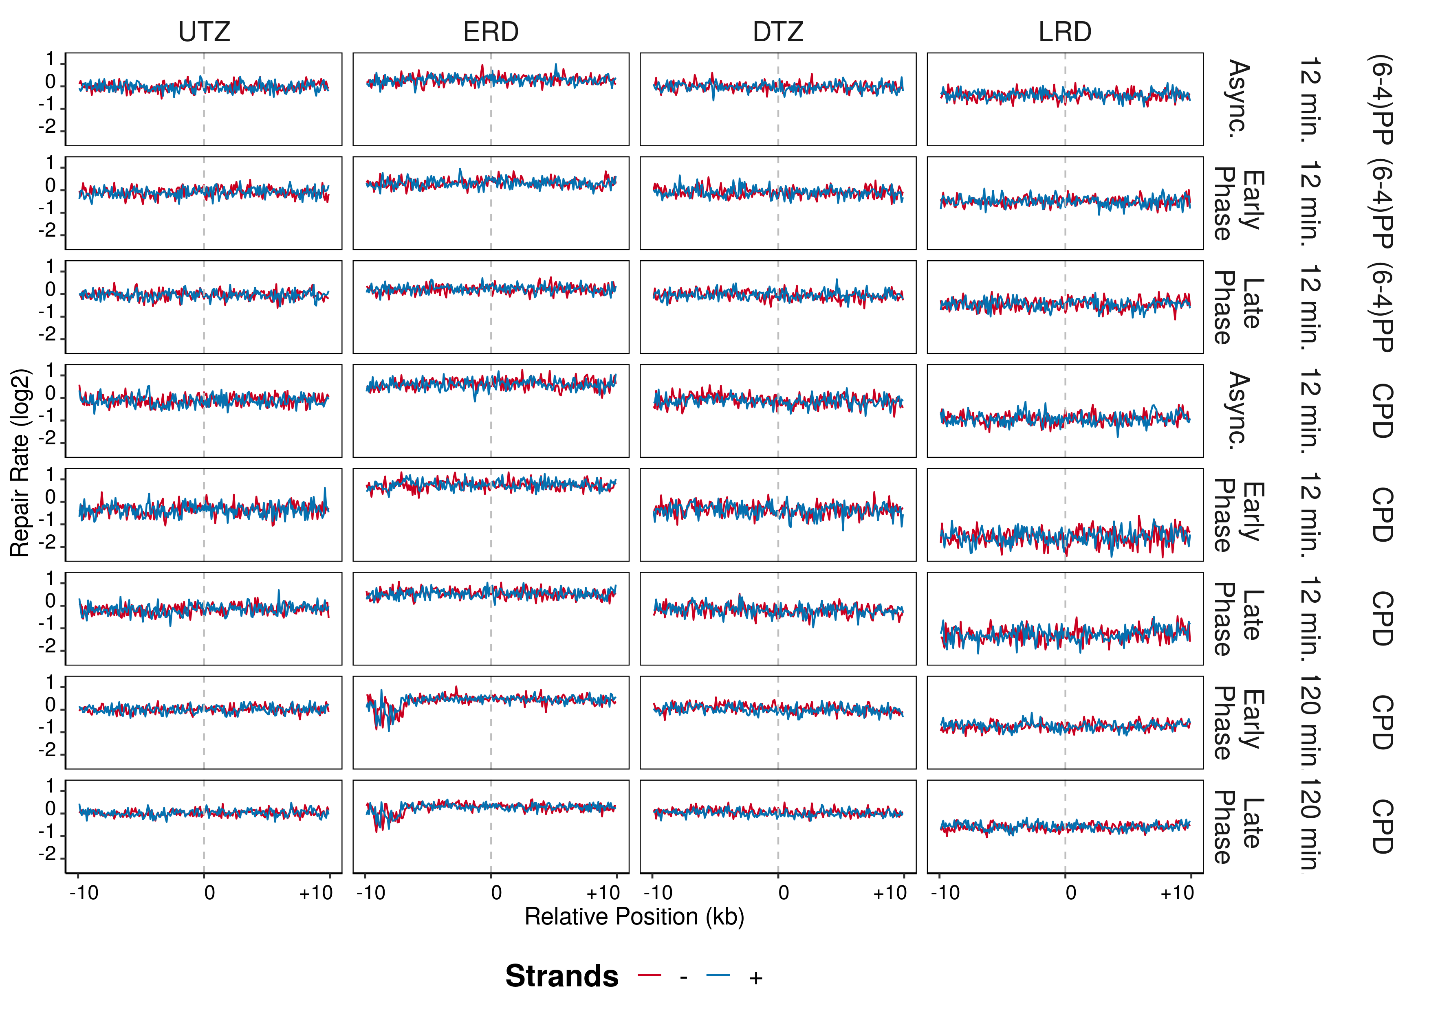
\includegraphics[width=\textwidth]{Chapters/7_appendix/figures/supfig18}
\caption[Repair rates of replication domains in 20 kb (replicate A).]{Repair rates (XR-seq/Damage-seq) are calculated and log2 transformed in 20 kb windows with 100 base pair intervals, which replication domains are positioned at the center of the region. The blue lines are the plus strands and red lines are the minus strands. Analysis is performed on replicate A.}
\label{supfig:repairrate20repdomainA}
\end{center}
\end{figure}

\begin{figure}[H]
\begin{center}
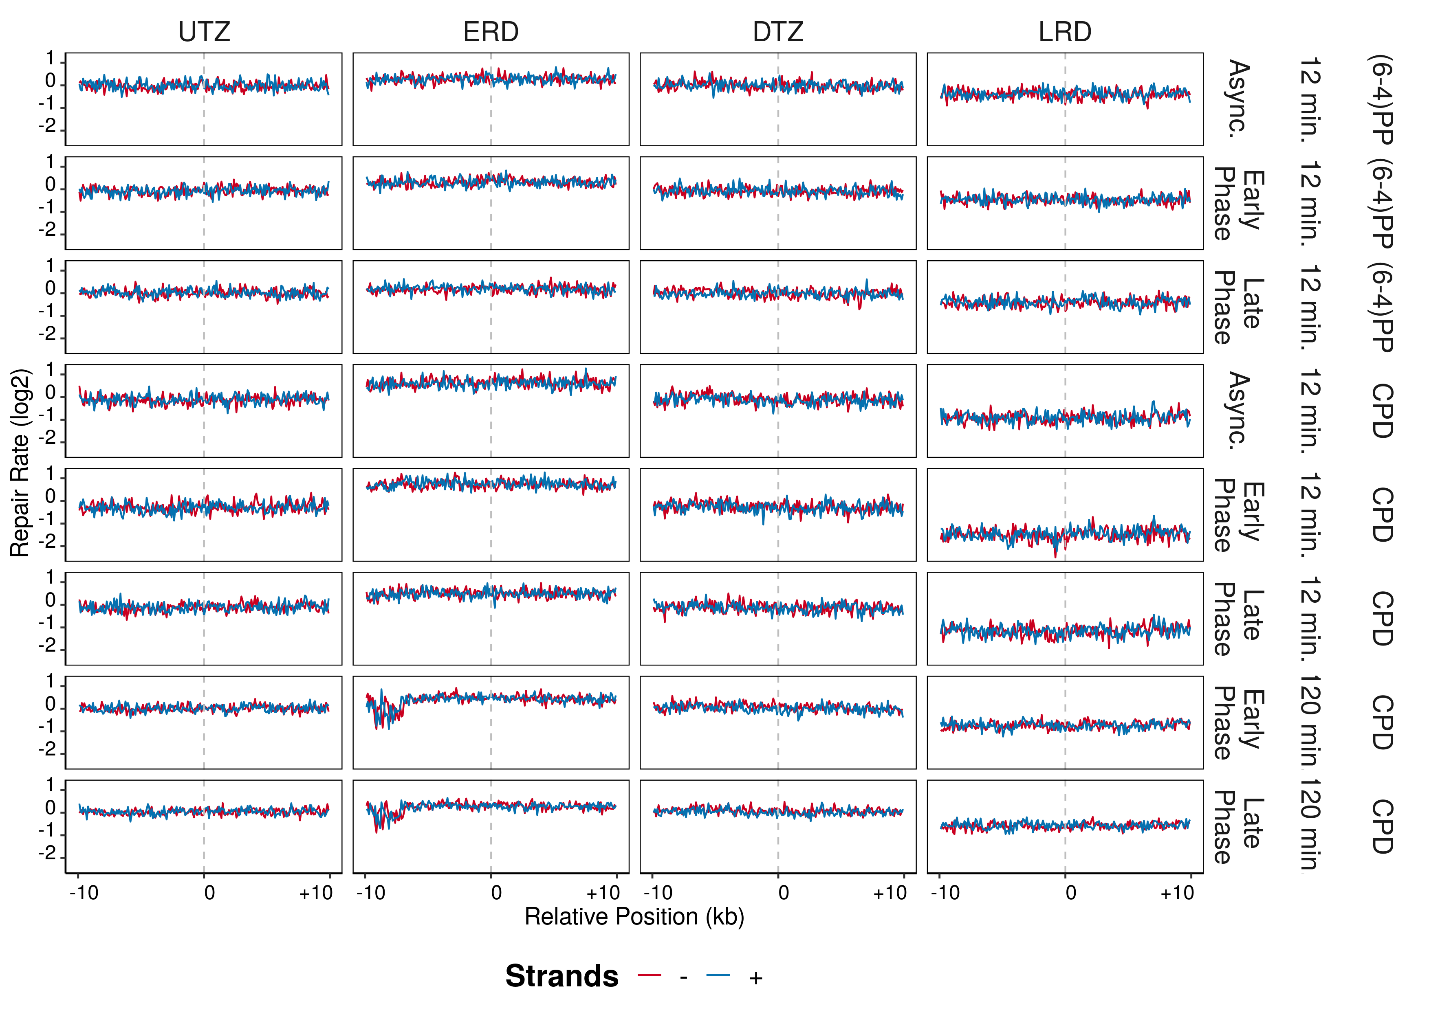
\includegraphics[width=\textwidth]{Chapters/7_appendix/figures/supfig19}
\caption[Repair rates of replication domains in 20 kb (replicate B).]{Repair rates (XR-seq/Damage-seq) are calculated and log2 transformed in 20 kb windows with 100 base pair intervals, which replication domains are positioned at the center of the region. The blue lines are the plus strands and red lines are the minus strands. Analysis is performed on replicate B.}
\label{supfig:repairrate20repdomainB}
\end{center}
\end{figure}

\begin{figure}[H]
\begin{center}
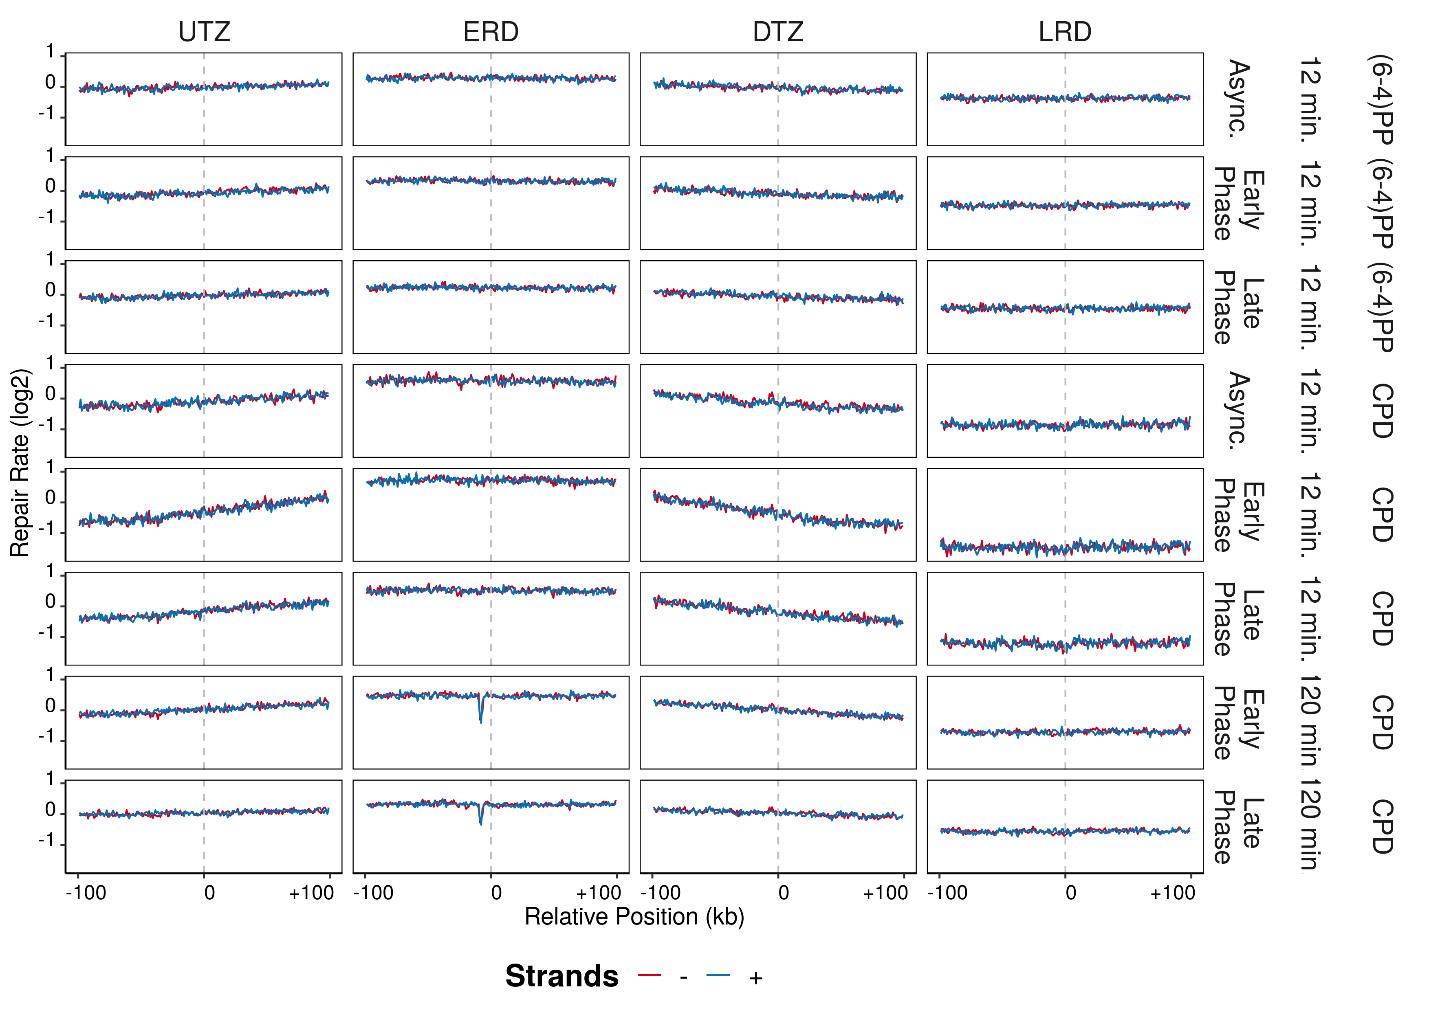
\includegraphics[width=\textwidth]{Chapters/7_appendix/figures/supfig20}
\caption[Repair rates of replication domains in 200 kb (replicate A).]{Repair rates (XR-seq/Damage-seq) are calculated and log2 transformed in 200 kb windows with 1 kb intervals, which replication domains are positioned at the center of the region. The blue lines are the plus strands and red lines are the minus strands. Analysis is performed on replicate A.}
\label{supfig:repairrate200repdomainA}
\end{center}
\end{figure}

\begin{figure}[H]
\begin{center}
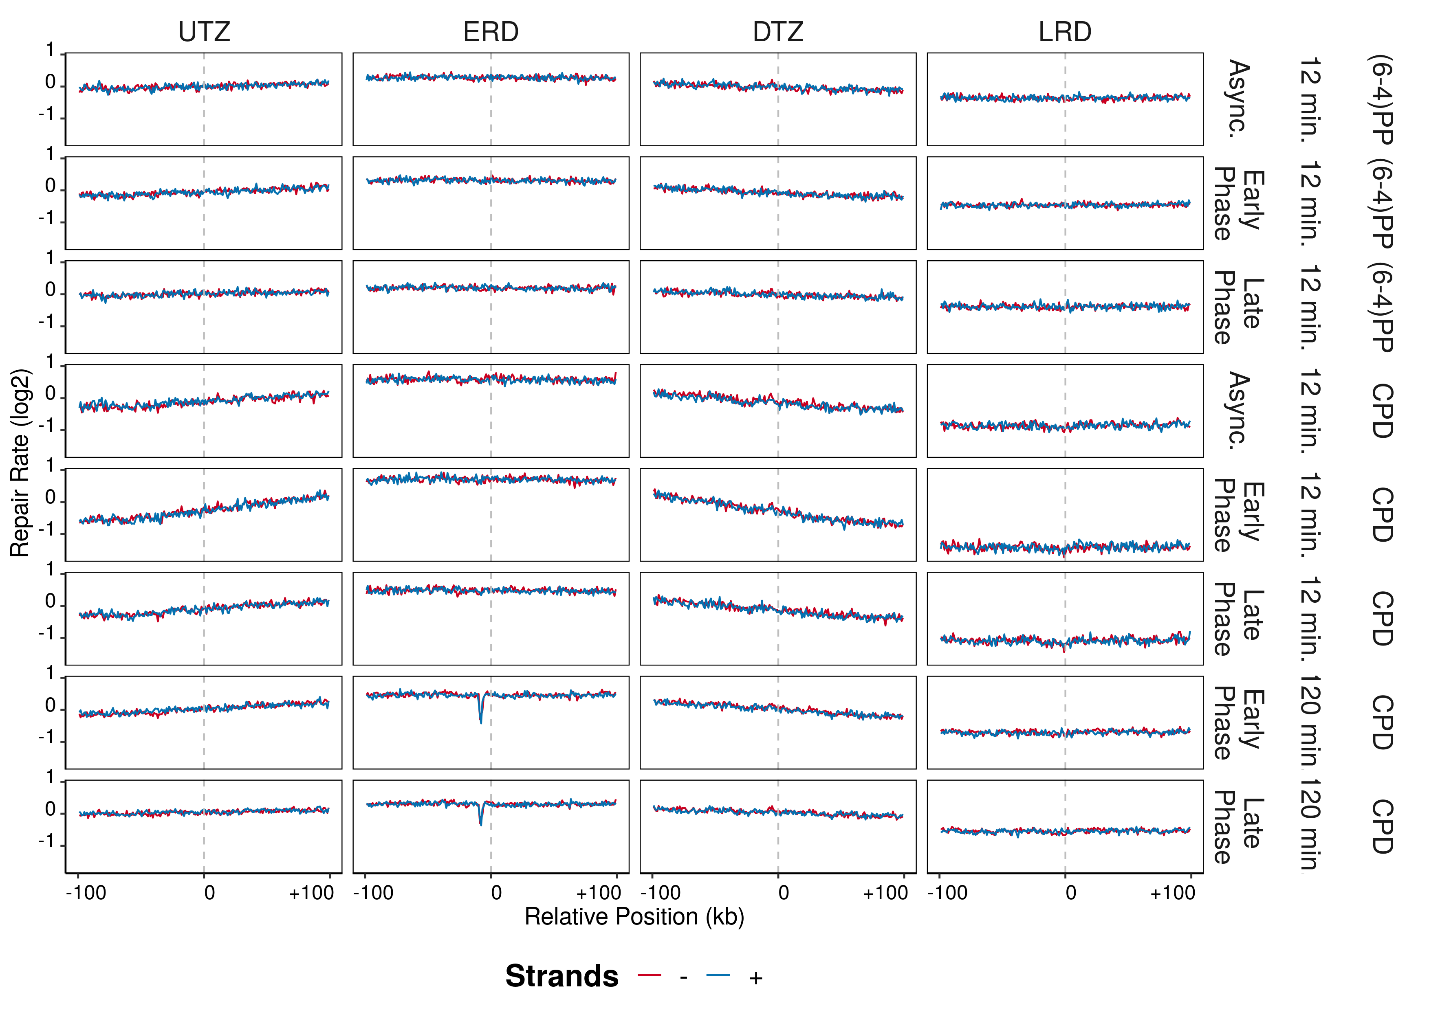
\includegraphics[width=\textwidth]{Chapters/7_appendix/figures/supfig21}
\caption[Repair rates of replication domains in 200 kb (replicate B).]{Repair rates (XR-seq/Damage-seq) are calculated and log2 transformed in 200 kb windows with 1 kb intervals, which replication domains are positioned at the center of the region. The blue lines are the plus strands and red lines are the minus strands. Analysis is performed on replicate B.}
\label{supfig:repairrate200repdomainB}
\end{center}
\end{figure}

\begin{figure}[H]
\begin{center}
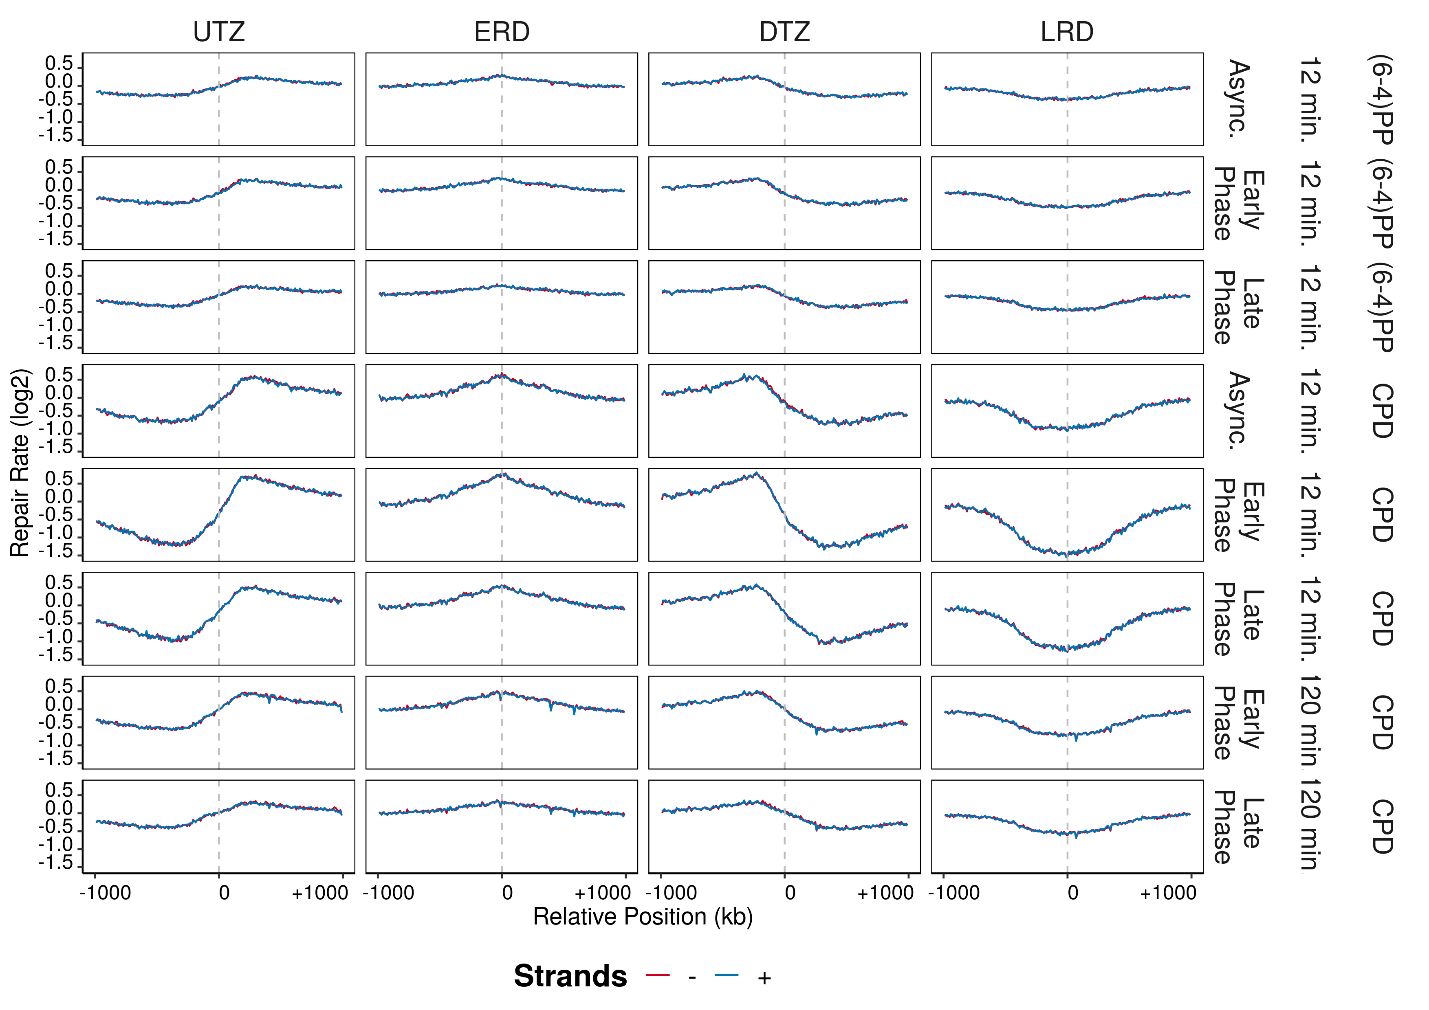
\includegraphics[width=\textwidth]{Chapters/7_appendix/figures/supfig22}
\caption[Repair rates of replication domains in 2 Mbp (replicate A).]{Repair rates (XR-seq/Damage-seq) are calculated and log2 transformed in 2 Mbp windows with 10 kb intervals, which replication domains are positioned at the center of the region. The blue lines are the plus strands and red lines are the minus strands. Analysis is performed on replicate A.}
\label{supfig:repairrate2000repdomainA}
\end{center}
\end{figure}

\begin{figure}[H]
\begin{center}
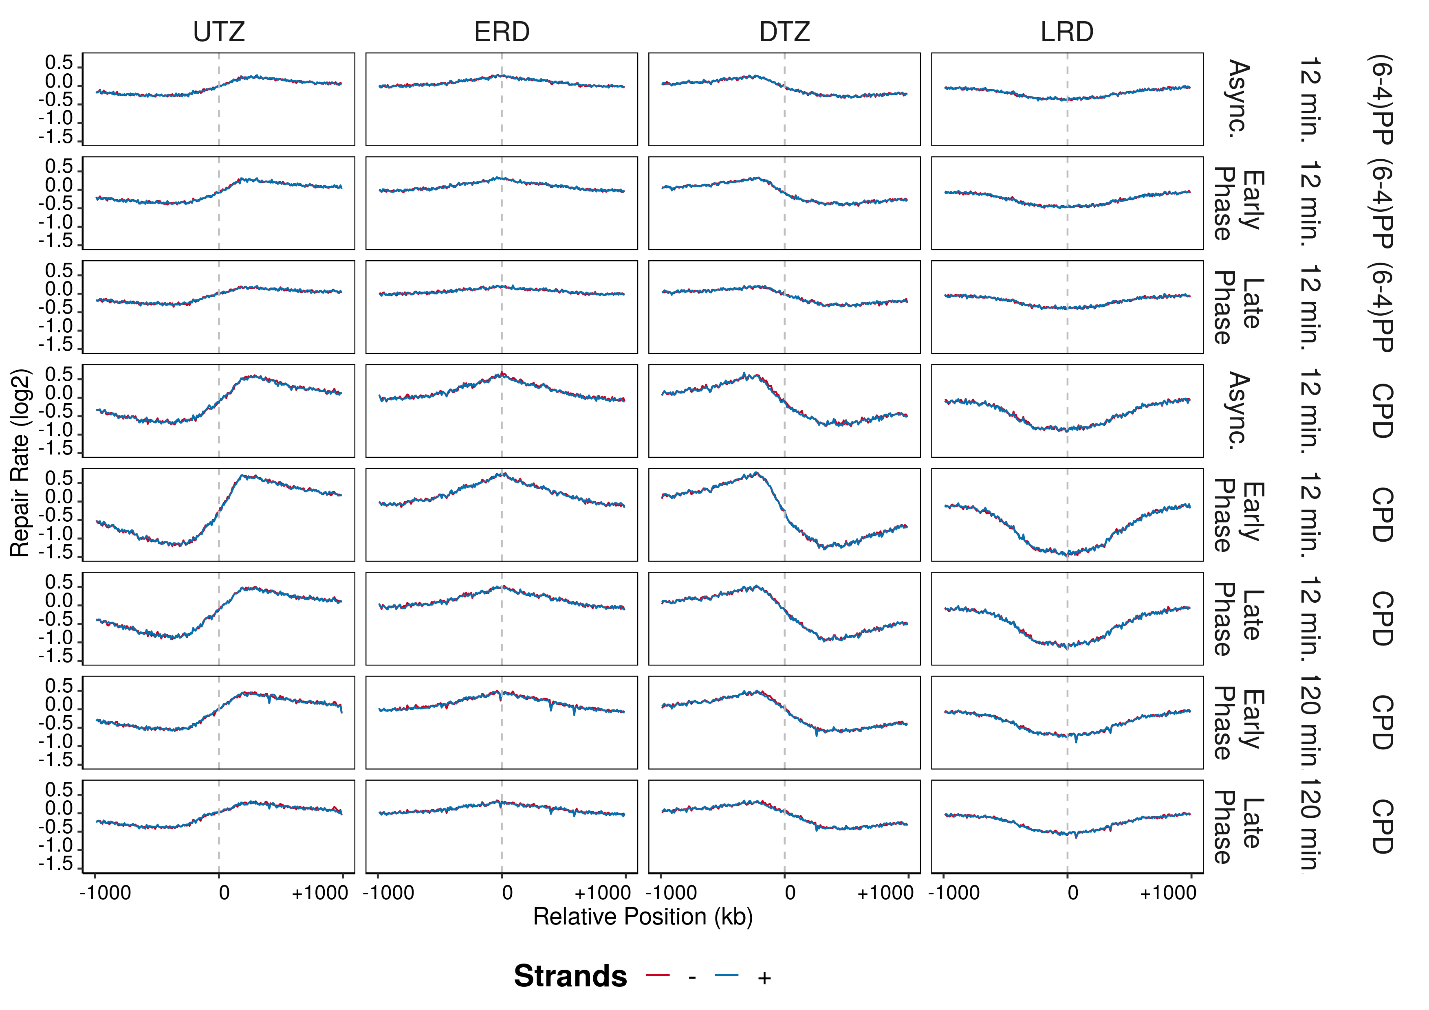
\includegraphics[width=\textwidth]{Chapters/7_appendix/figures/supfig23}
\caption[Repair rates of replication domains in 2 Mbp (replicate B).]{Repair rates (XR-seq/Damage-seq) are calculated and log2 transformed in 2 Mbp windows with 10 kb intervals, which replication domains are positioned at the center of the region. The blue lines are the plus strands and red lines are the minus strands. Analysis is performed on replicate B.}
\label{supfig:repairrate2000repdomainB}
\end{center}
\end{figure}

\begin{figure}[H]
\begin{center}
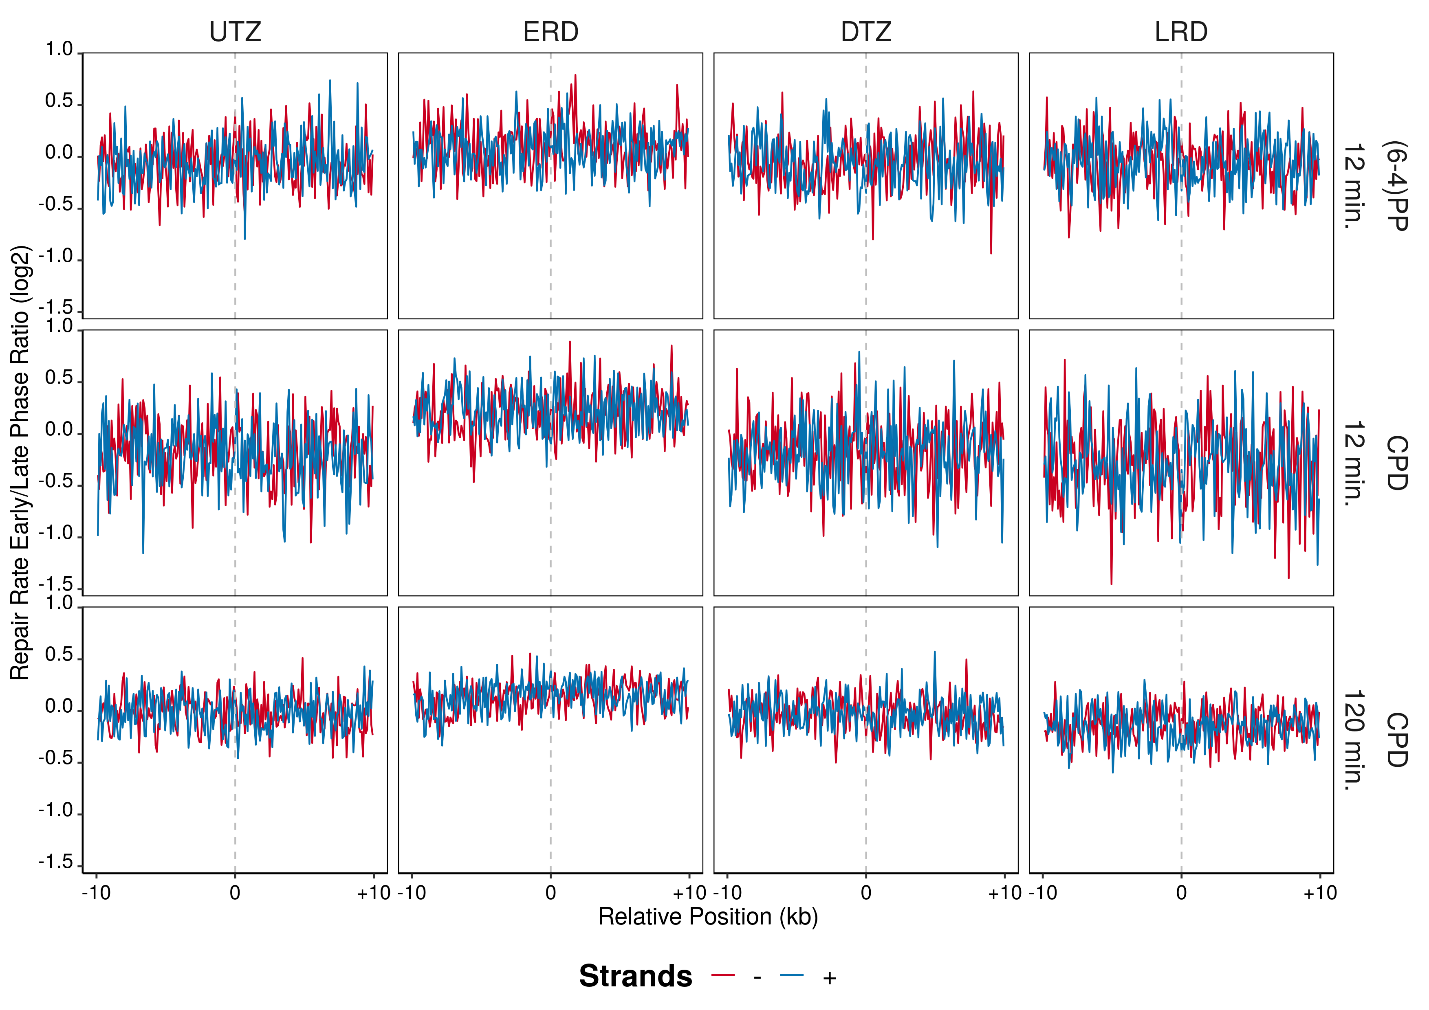
\includegraphics[width=\textwidth]{Chapters/7_appendix/figures/supfig24}
\caption[Repair rate early/late phase ratio of replication domains in 20 kb (replicate A).]{After log2 transformed repair rates (XR-seq/Damage-seq) are calculated, samples that are at early S phase of the cell cycle are further divided by the ones that are at the late S phase (early/late) in 20 kb windows with 100 base pair intervals, which replication domains are positioned at the center of the region. The blue lines are the plus strands and red lines are the minus strands. Analysis is performed on replicate A.}
\label{supfig:rrel20repdomainA}
\end{center}
\end{figure}

\begin{figure}[H]
\begin{center}
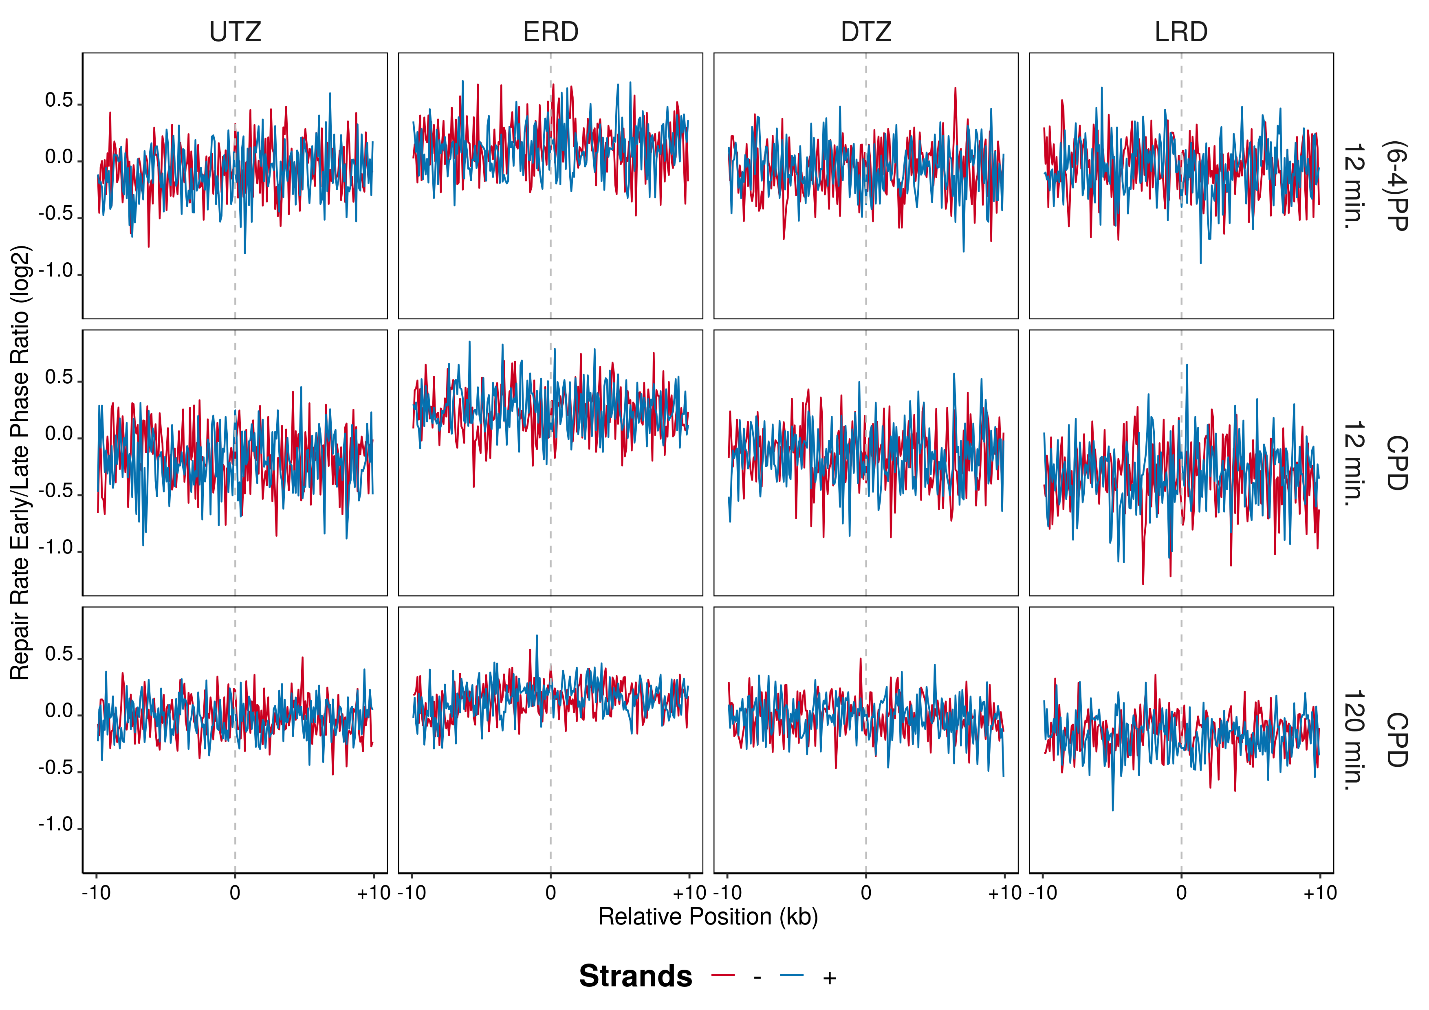
\includegraphics[width=\textwidth]{Chapters/7_appendix/figures/supfig25}
\caption[Repair rate early/late phase ratio of replication domains in 20 kb (replicate B).]{After log2 transformed repair rates (XR-seq/Damage-seq) are calculated, samples that are at early S phase of the cell cycle are further divided by the ones that are at the late S phase (early/late) in 20 kb windows with 100 base pair intervals, which replication domains are positioned at the center of the region. The blue lines are the plus strands and red lines are the minus strands. Analysis is performed on replicate B.}
\label{supfig:rrel20repdomainB}
\end{center}
\end{figure}

\begin{figure}[H]
\begin{center}
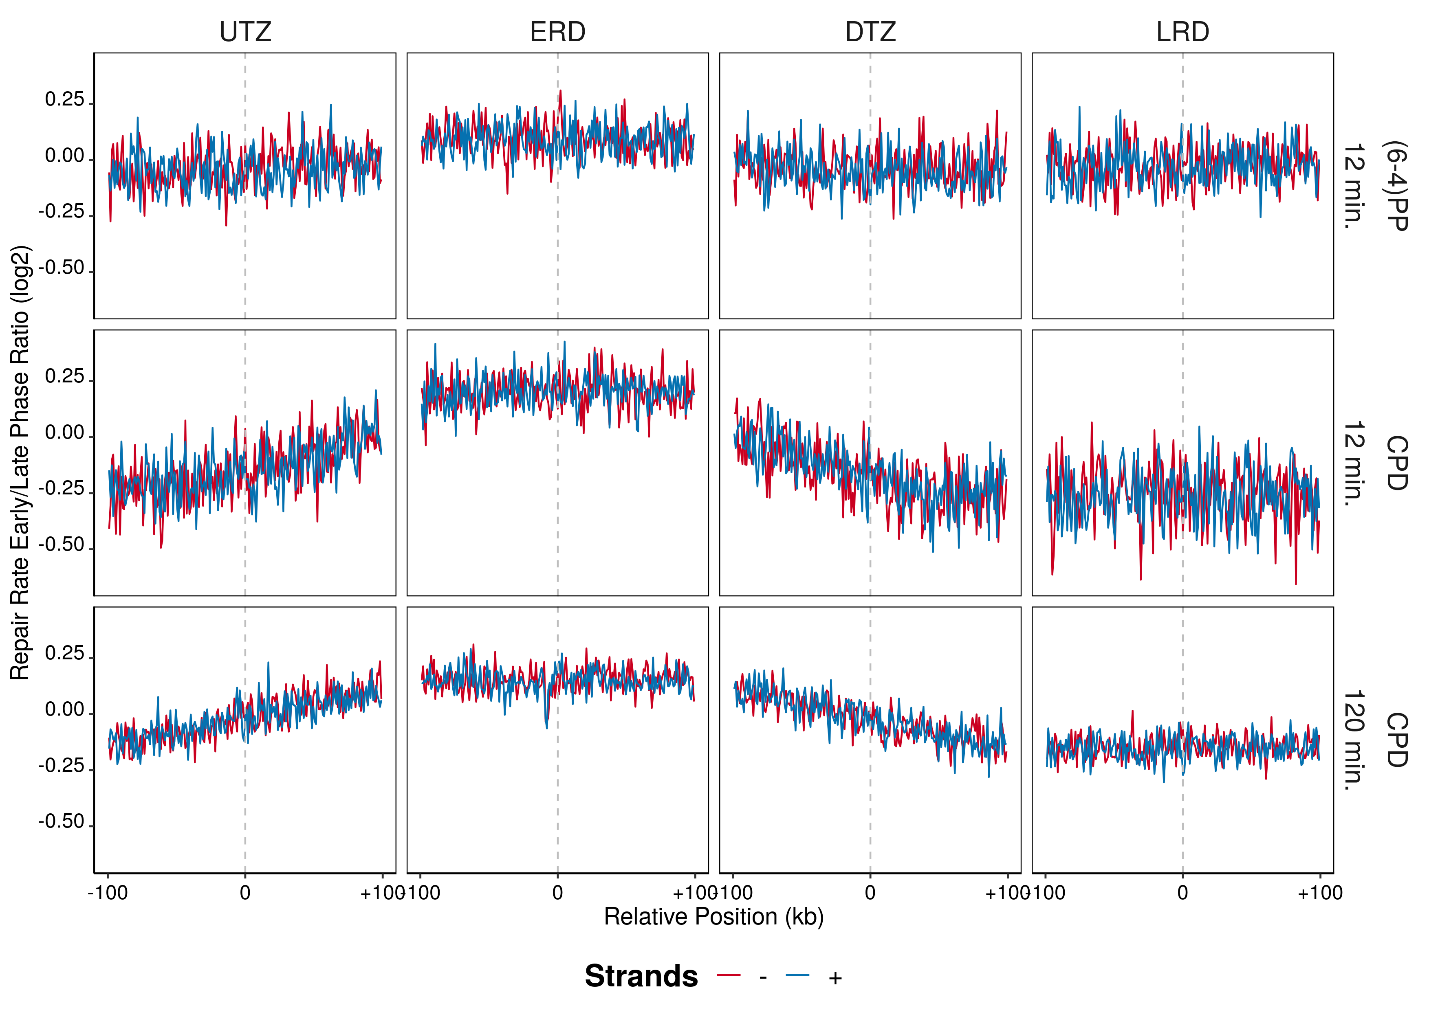
\includegraphics[width=\textwidth]{Chapters/7_appendix/figures/supfig26}
\caption[Repair rate early/late phase ratio of replication domains in 200 kb (replicate A).]{After log2 transformed repair rates (XR-seq/Damage-seq) are calculated, samples that are at early S phase of the cell cycle are further divided by the ones that are at the late S phase (early/late) in 200 kb windows with 1 kb intervals, which replication domains are positioned at the center of the region. The blue lines are the plus strands and red lines are the minus strands. Analysis is performed on replicate A.}
\label{supfig:rrel200repdomainA}
\end{center}
\end{figure}

\begin{figure}[H]
\begin{center}
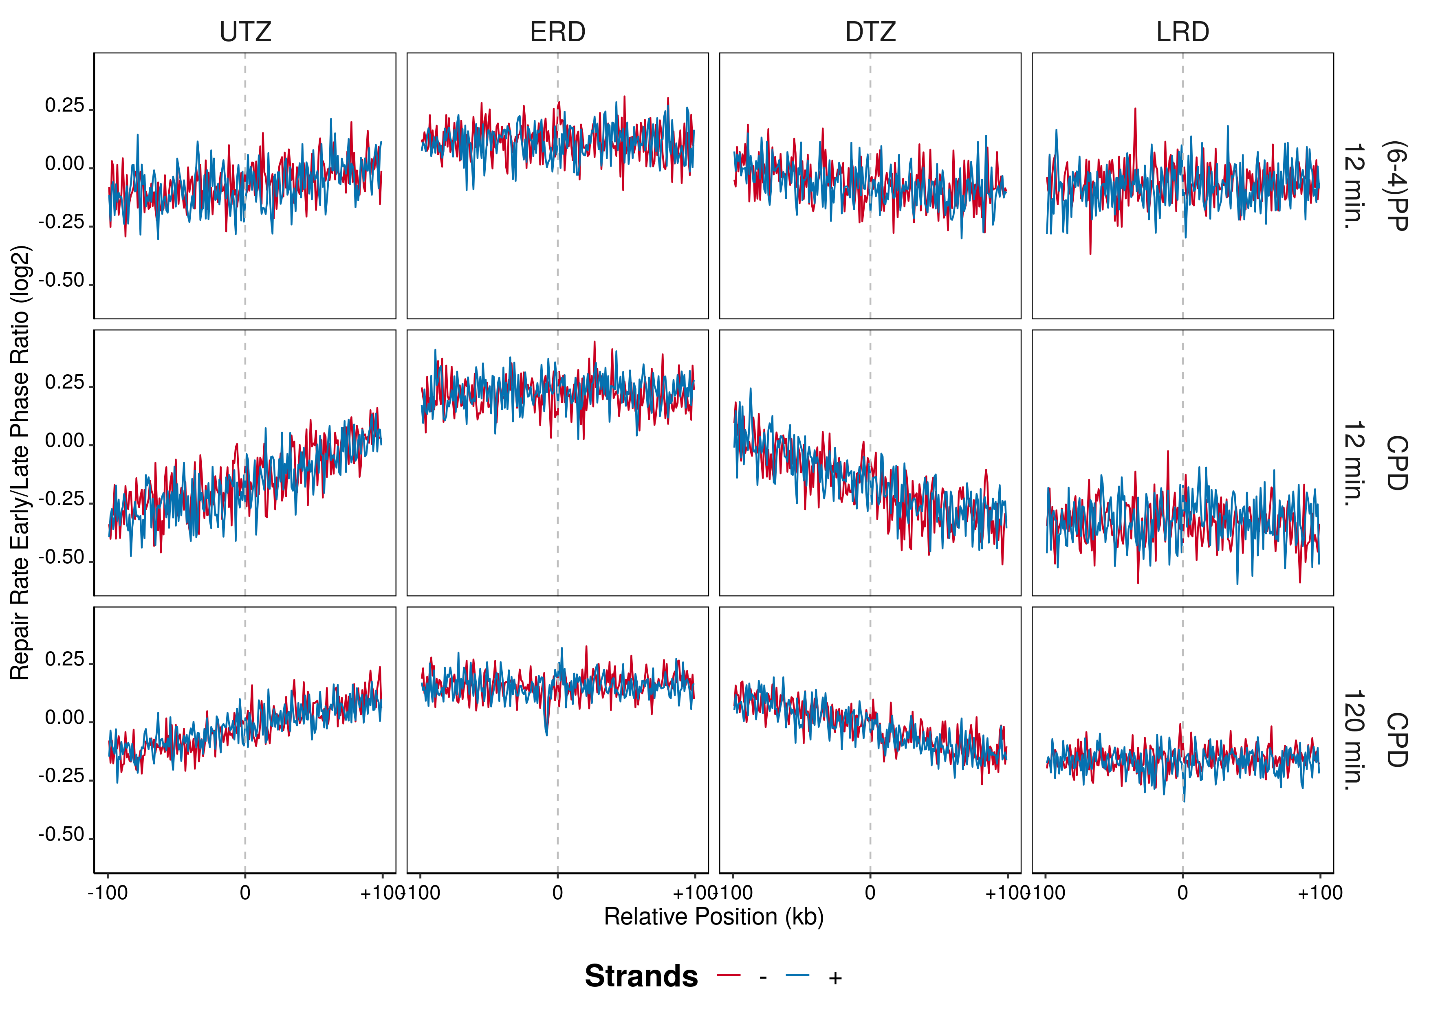
\includegraphics[width=\textwidth]{Chapters/7_appendix/figures/supfig27}
\caption[Repair rate early/late phase ratio of replication domains in 200 kb (replicate B).]{After log2 transformed repair rates (XR-seq/Damage-seq) are calculated, samples that are at early S phase of the cell cycle are further divided by the ones that are at the late S phase (early/late) in 200 kb windows with 1 kb intervals, which replication domains are positioned at the center of the region. The blue lines are the plus strands and red lines are the minus strands. Analysis is performed on replicate B.}
\label{supfig:rrel200repdomainB}
\end{center}
\end{figure}

\begin{figure}[H]
\begin{center}
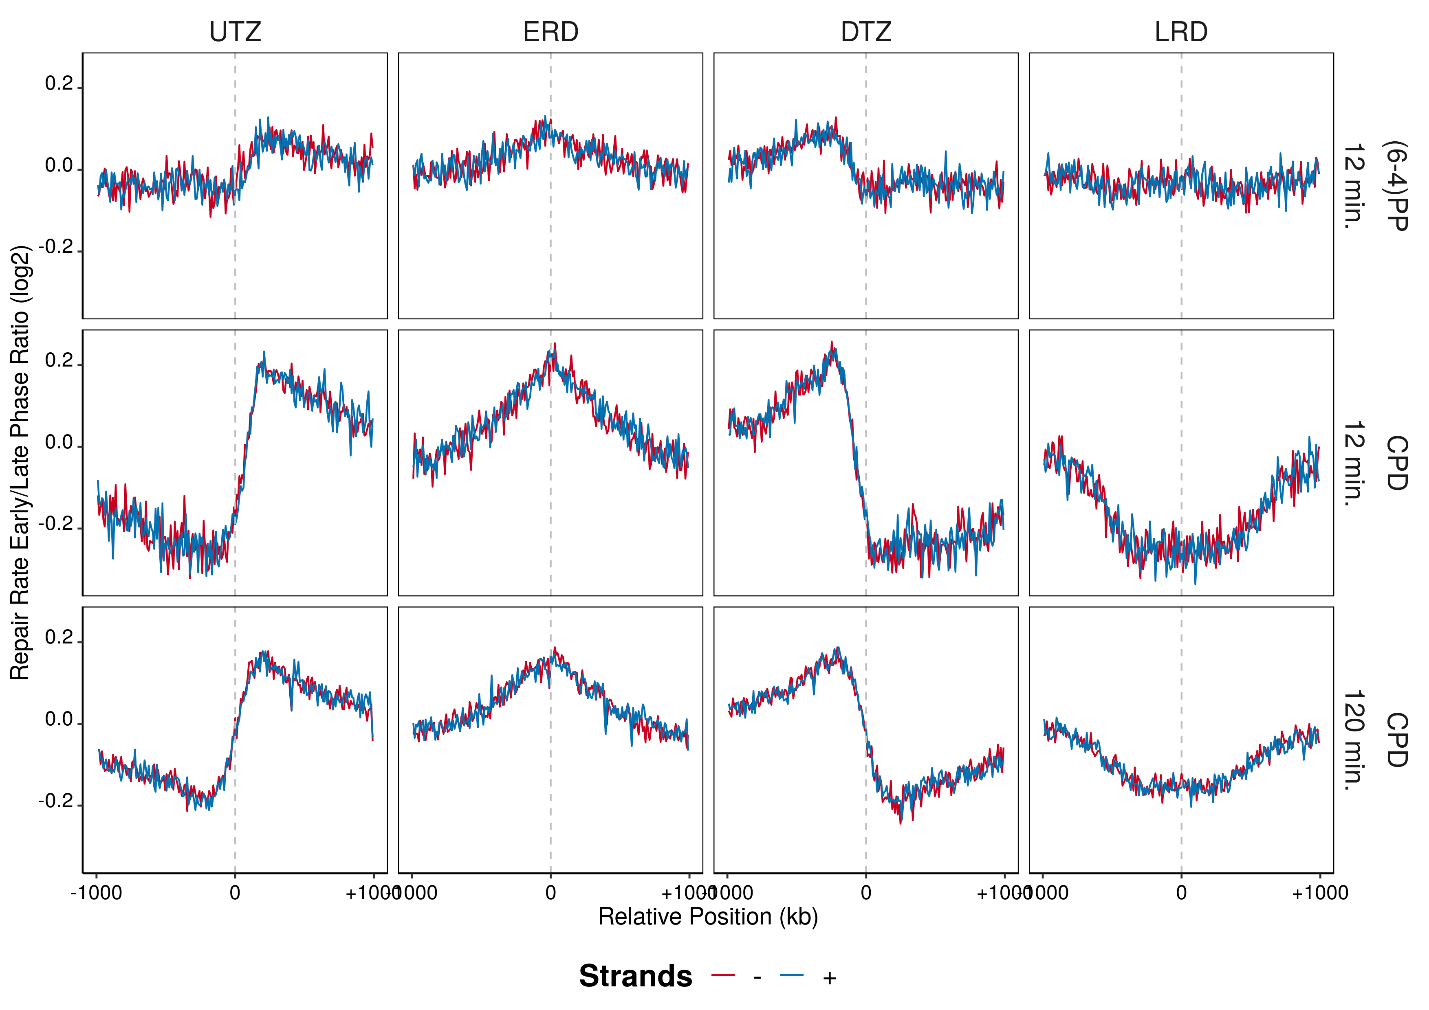
\includegraphics[width=\textwidth]{Chapters/7_appendix/figures/supfig28}
\caption[Repair rate early/late phase ratio of replication domains in 2 Mbp (replicate A).]{After log2 transformed repair rates (XR-seq/Damage-seq) are calculated, samples that are at early S phase of the cell cycle are further divided by the ones that are at the late S phase (early/late) in 2 Mbp windows with 10 kb intervals, which replication domains are positioned at the center of the region. The blue lines are the plus strands and red lines are the minus strands. Analysis is performed on replicate A.}
\label{supfig:rrel2000repdomainA}
\end{center}
\end{figure}

\begin{figure}[H]
\begin{center}
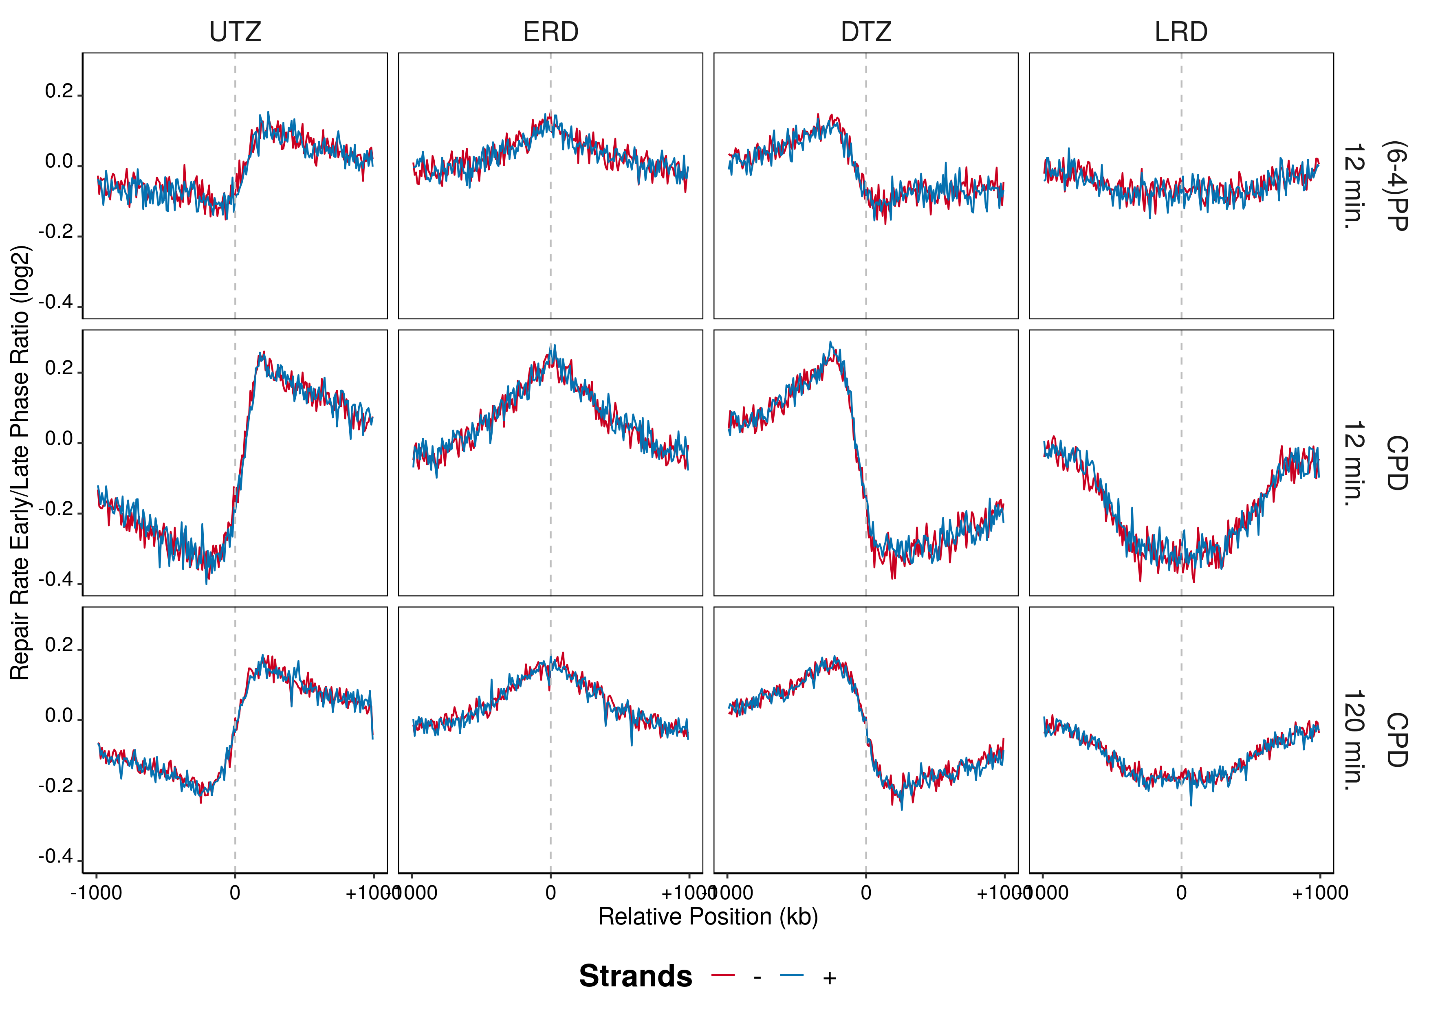
\includegraphics[width=\textwidth]{Chapters/7_appendix/figures/supfig29}
\caption[Repair rate early/late phase ratio of replication domains in 2 Mbp (replicate B).]{After log2 transformed repair rates (XR-seq/Damage-seq) are calculated, samples that are at early S phase of the cell cycle are further divided by the ones that are at the late S phase (early/late) in 2 Mbp windows with 10 kb intervals, which replication domains are positioned at the center of the region. The blue lines are the plus strands and red lines are the minus strands. Analysis is performed on replicate B.}
\label{supfig:rrel2000repdomainB}
\end{center}
\end{figure}

\begin{figure}[H]
\begin{center}
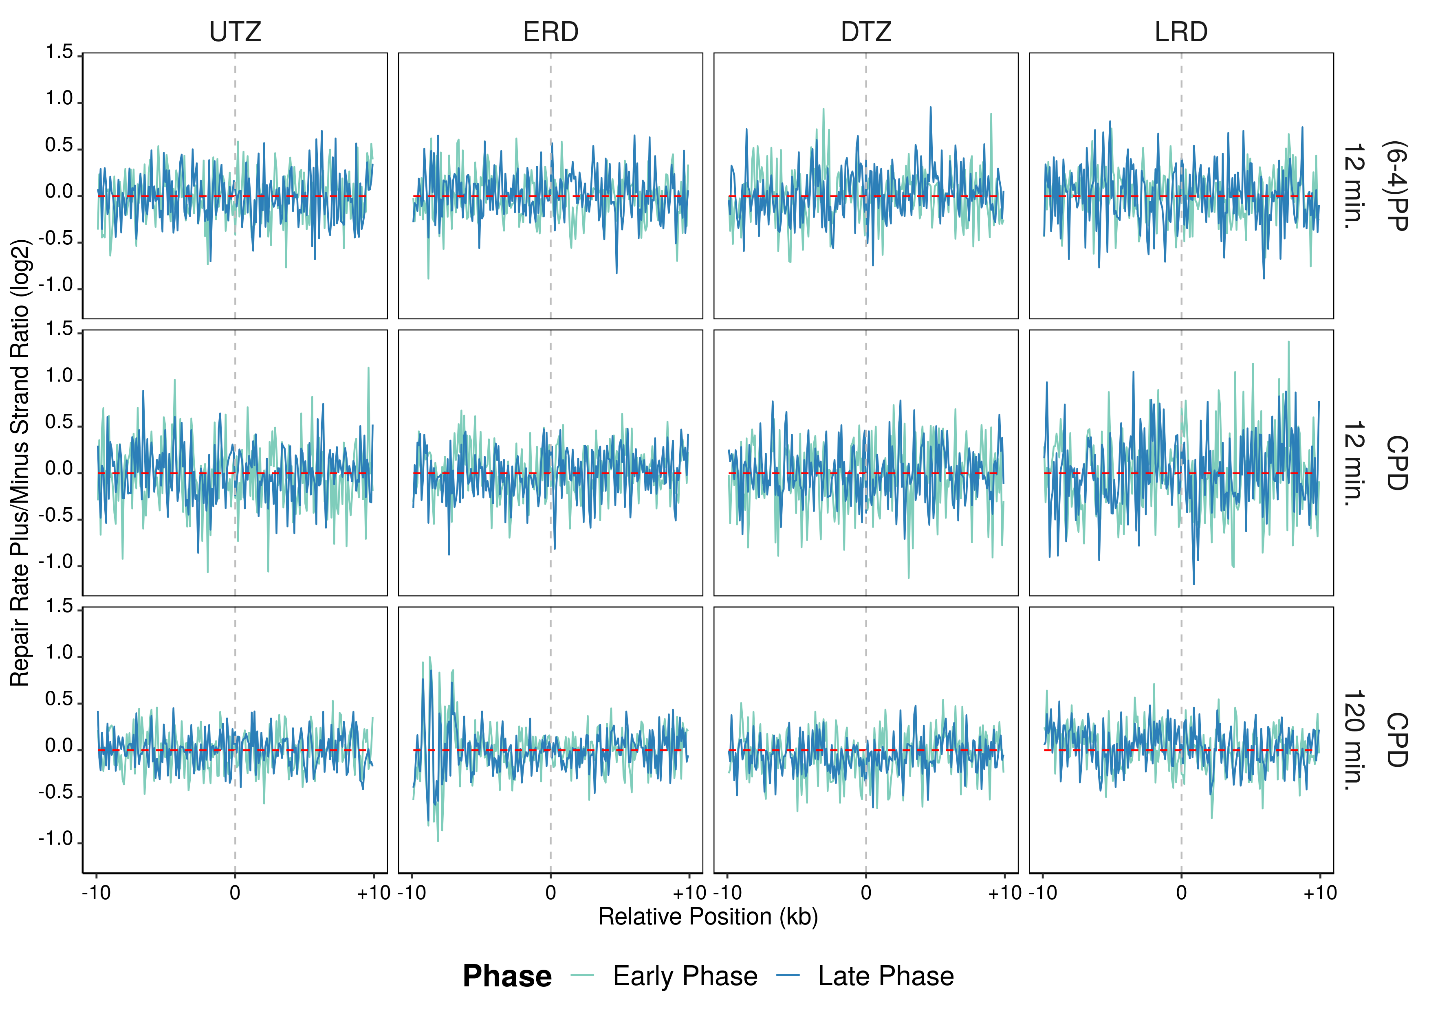
\includegraphics[width=\textwidth]{Chapters/7_appendix/figures/supfig30}
\caption[Repair rate plus/minus phase ratio of replication domains in 20 kb (replicate A).]{After log2 transformed repair rates (XR-seq/Damage-seq) are calculated, plus strands of the samples are further divided to minus strands (plus/minus) in 20 kb windows with 100 base pair intervals, which replication domains are positioned at the center of the region. Light blue lines are the early phase samples and dark blue lines are the late phase samples. Analysis is performed on replicate A.}
\label{supfig:rrpm20repdomainA}
\end{center}
\end{figure}

\begin{figure}[H]
\begin{center}
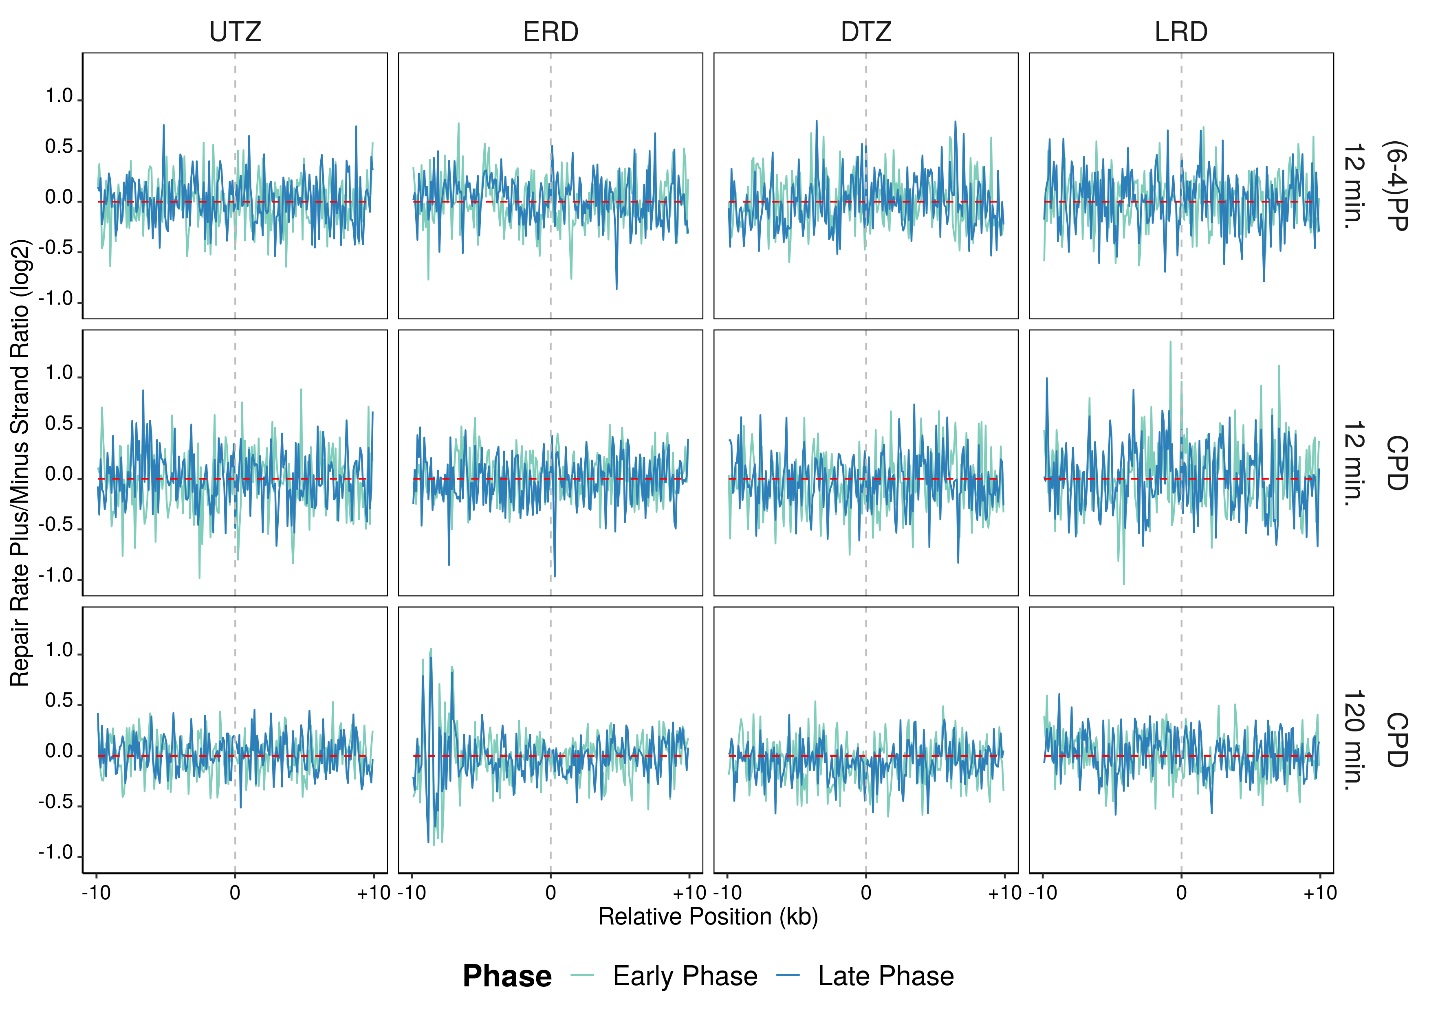
\includegraphics[width=\textwidth]{Chapters/7_appendix/figures/supfig31}
\caption[Repair rate plus/minus phase ratio of replication domains in 20 kb (replicate B).]{After log2 transformed repair rates (XR-seq/Damage-seq) are calculated, plus strands of the samples are further divided to minus strands (plus/minus) in 20 kb windows with 100 base pair intervals, which replication domains are positioned at the center of the region. Light blue lines are the early phase samples and dark blue lines are the late phase samples. Analysis is performed on replicate B.}
\label{supfig:rrpm20repdomainB}
\end{center}
\end{figure}

\begin{figure}[H]
\begin{center}
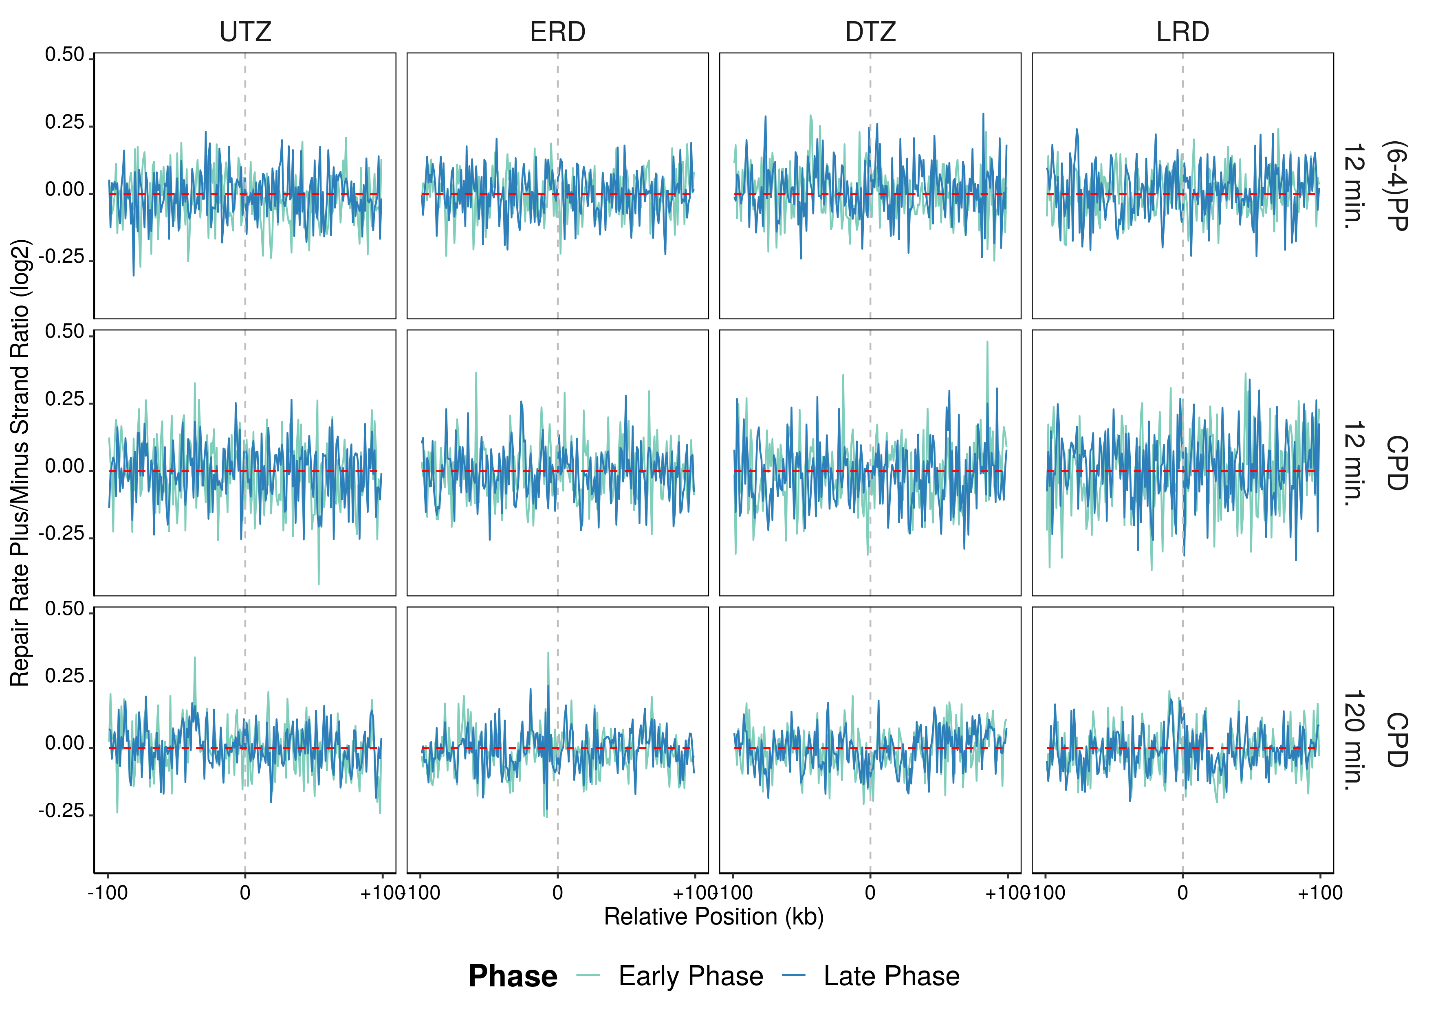
\includegraphics[width=\textwidth]{Chapters/7_appendix/figures/supfig32}
\caption[Repair rate plus/minus phase ratio of replication domains in 200 kb (replicate A).]{After log2 transformed repair rates (XR-seq/Damage-seq) are calculated, plus strands of the samples are further divided to minus strands (plus/minus) in 200 kb windows with 1 kb intervals, which replication domains are positioned at the center of the region. Light blue lines are the early phase samples and dark blue lines are the late phase samples. Analysis is performed on replicate A.}
\label{supfig:rrpm200repdomainA}
\end{center}
\end{figure}

\begin{figure}[H]
\begin{center}
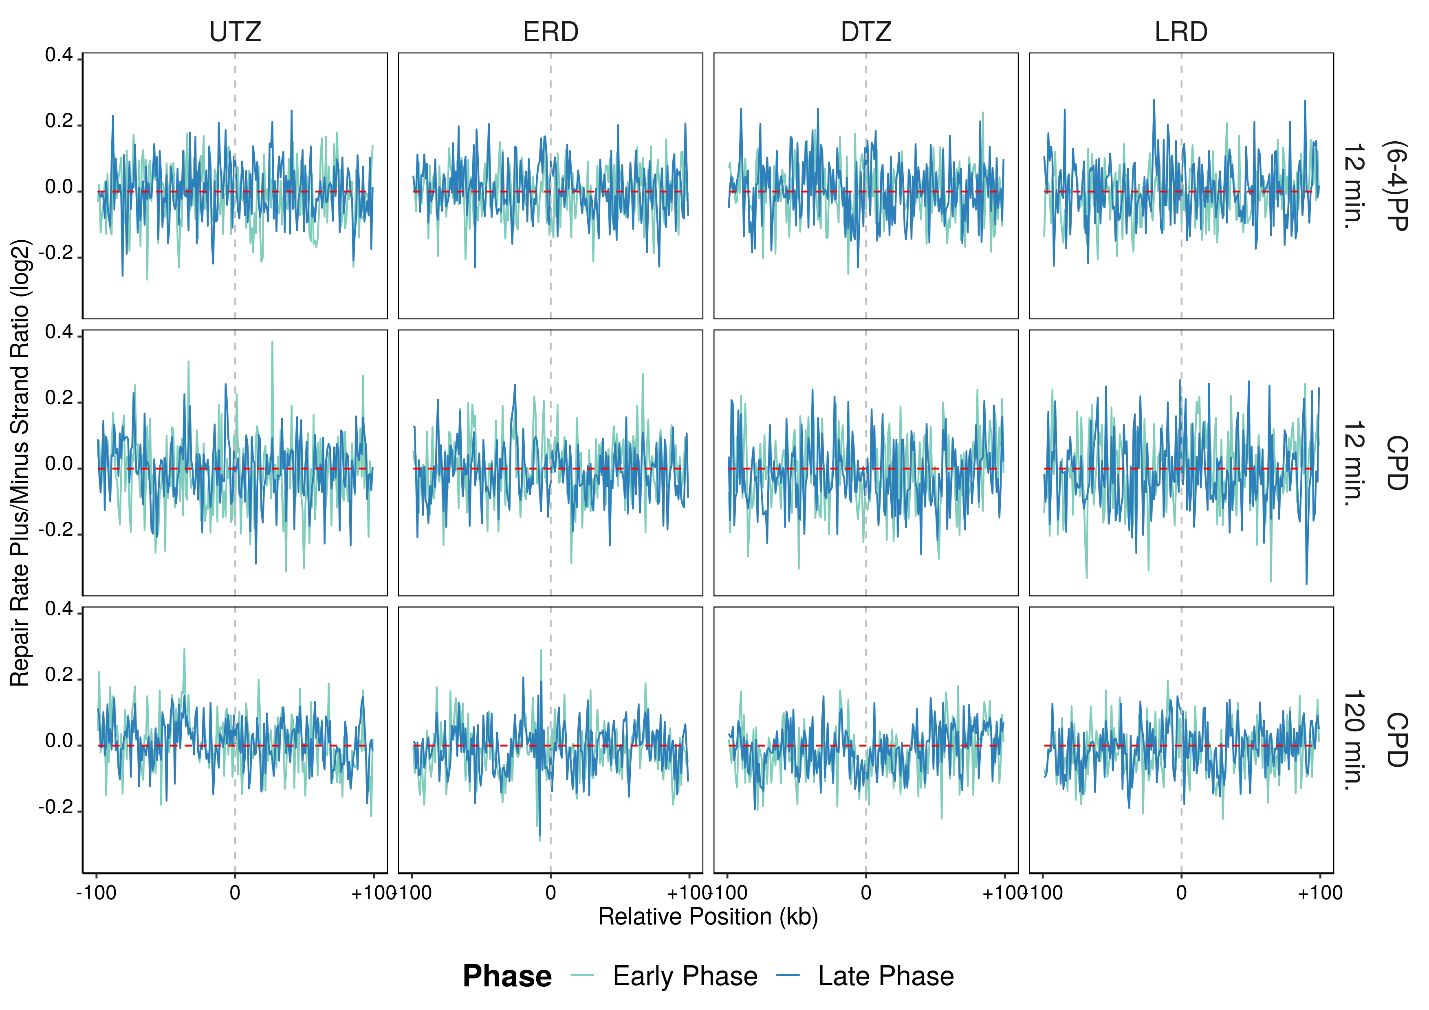
\includegraphics[width=\textwidth]{Chapters/7_appendix/figures/supfig33}
\caption[Repair rate plus/minus phase ratio of replication domains in 200 kb (replicate B).]{After log2 transformed repair rates (XR-seq/Damage-seq) are calculated, plus strands of the samples are further divided to minus strands (plus/minus) in 200 kb windows with 1 kb intervals, which replication domains are positioned at the center of the region. Light blue lines are the early phase samples and dark blue lines are the late phase samples. Analysis is performed on replicate B.}
\label{supfig:rrpm200repdomainB}
\end{center}
\end{figure}

\begin{figure}[H]
\begin{center}
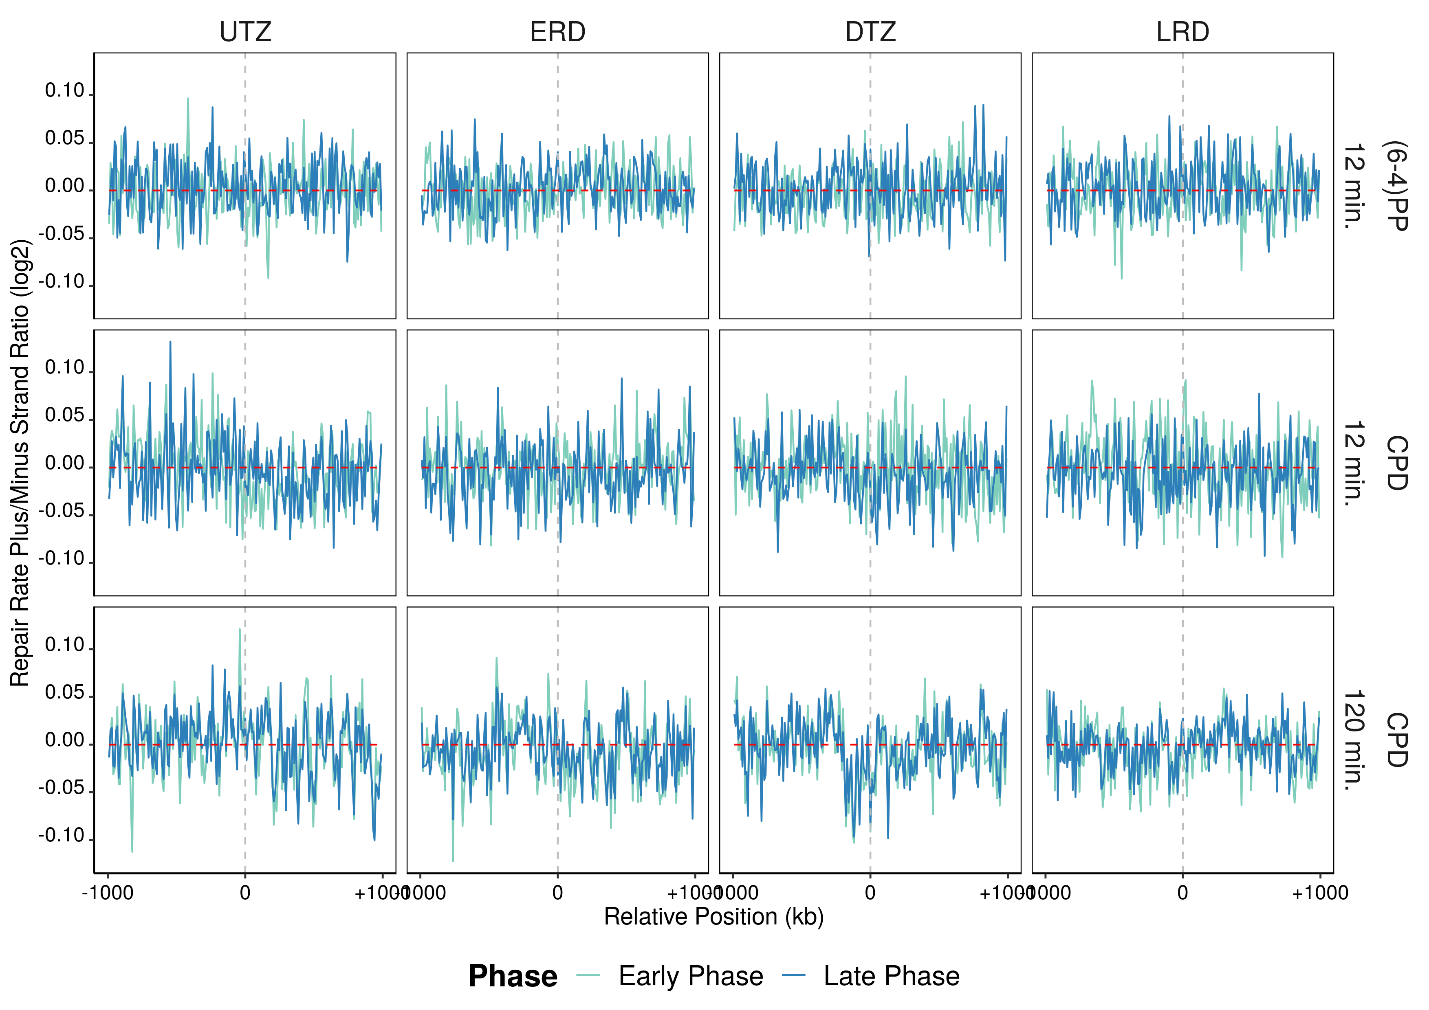
\includegraphics[width=\textwidth]{Chapters/7_appendix/figures/supfig34}
\caption[Repair rate plus/minus phase ratio of replication domains in 2 Mbp (replicate A).]{After log2 transformed repair rates (XR-seq/Damage-seq) are calculated, plus strands of the samples are further divided to minus strands (plus/minus) in 2 Mbp windows with 10 kb intervals, which replication domains are positioned at the center of the region. Light blue lines are the early phase samples and dark blue lines are the late phase samples. Analysis is performed on replicate A.}
\label{supfig:rrpm2000repdomainA}
\end{center}
\end{figure}

\begin{figure}[H]
\begin{center}
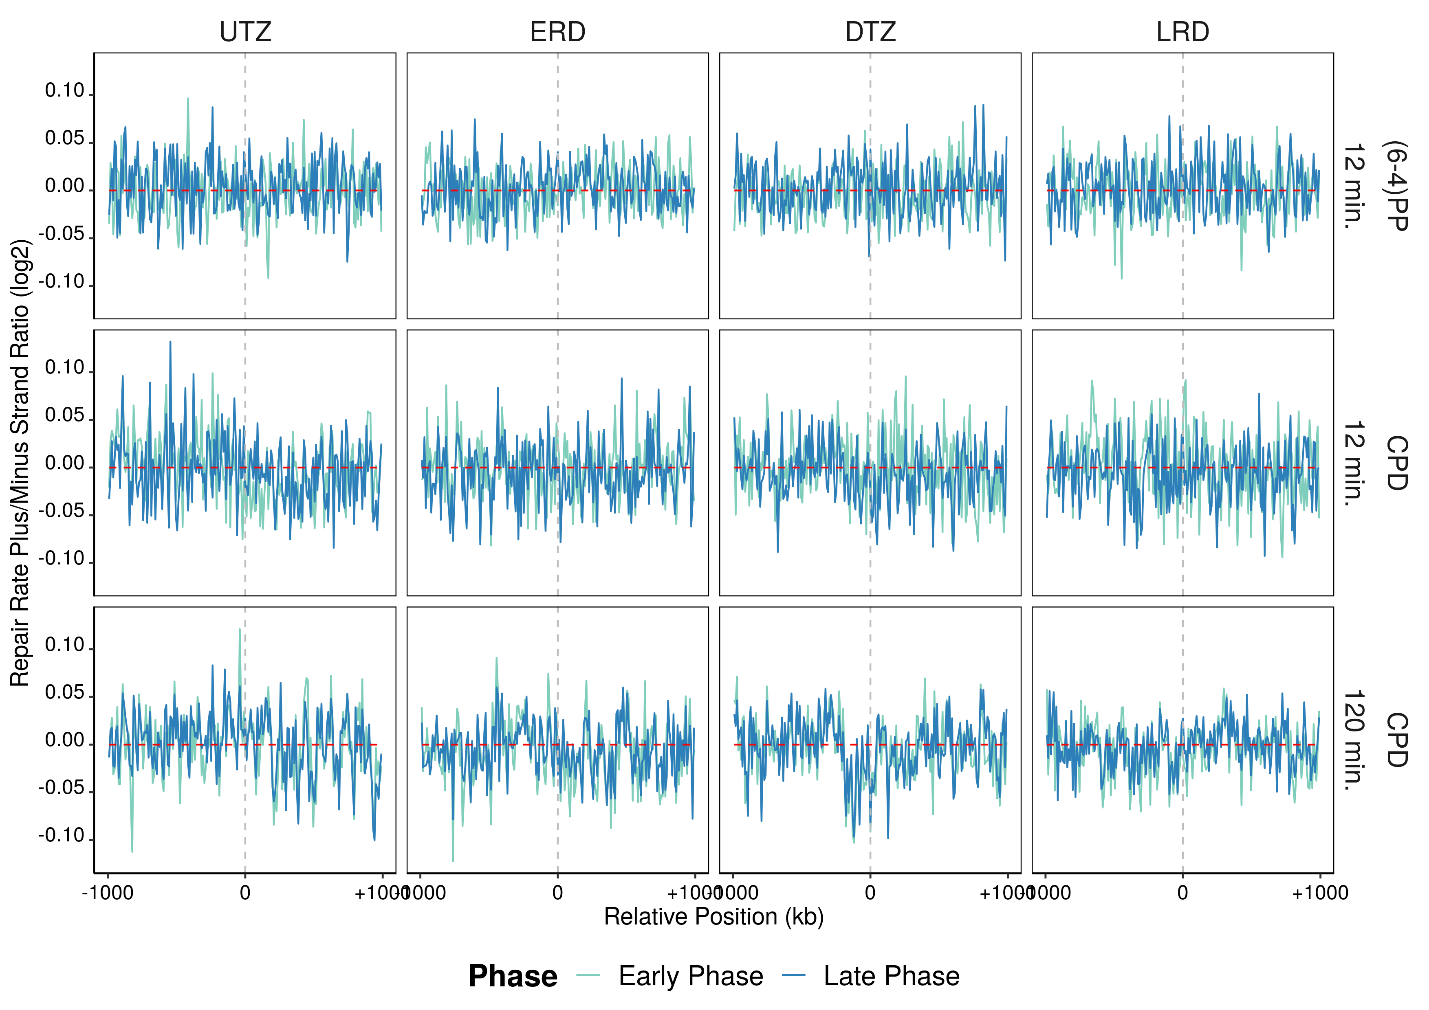
\includegraphics[width=\textwidth]{Chapters/7_appendix/figures/supfig35}
\caption[Repair rate plus/minus phase ratio of replication domains in 2 Mbp (replicate B).]{After log2 transformed repair rates (XR-seq/Damage-seq) are calculated, plus strands of the samples are further divided to minus strands (plus/minus) in 2 Mbp windows with 10 kb intervals, which replication domains are positioned at the center of the region. Light blue lines are the early phase samples and dark blue lines are the late phase samples. Analysis is performed on replicate B.}
\label{supfig:rrpm2000repdomainB}
\end{center}
\end{figure}

\begin{figure}[H]
\begin{center}
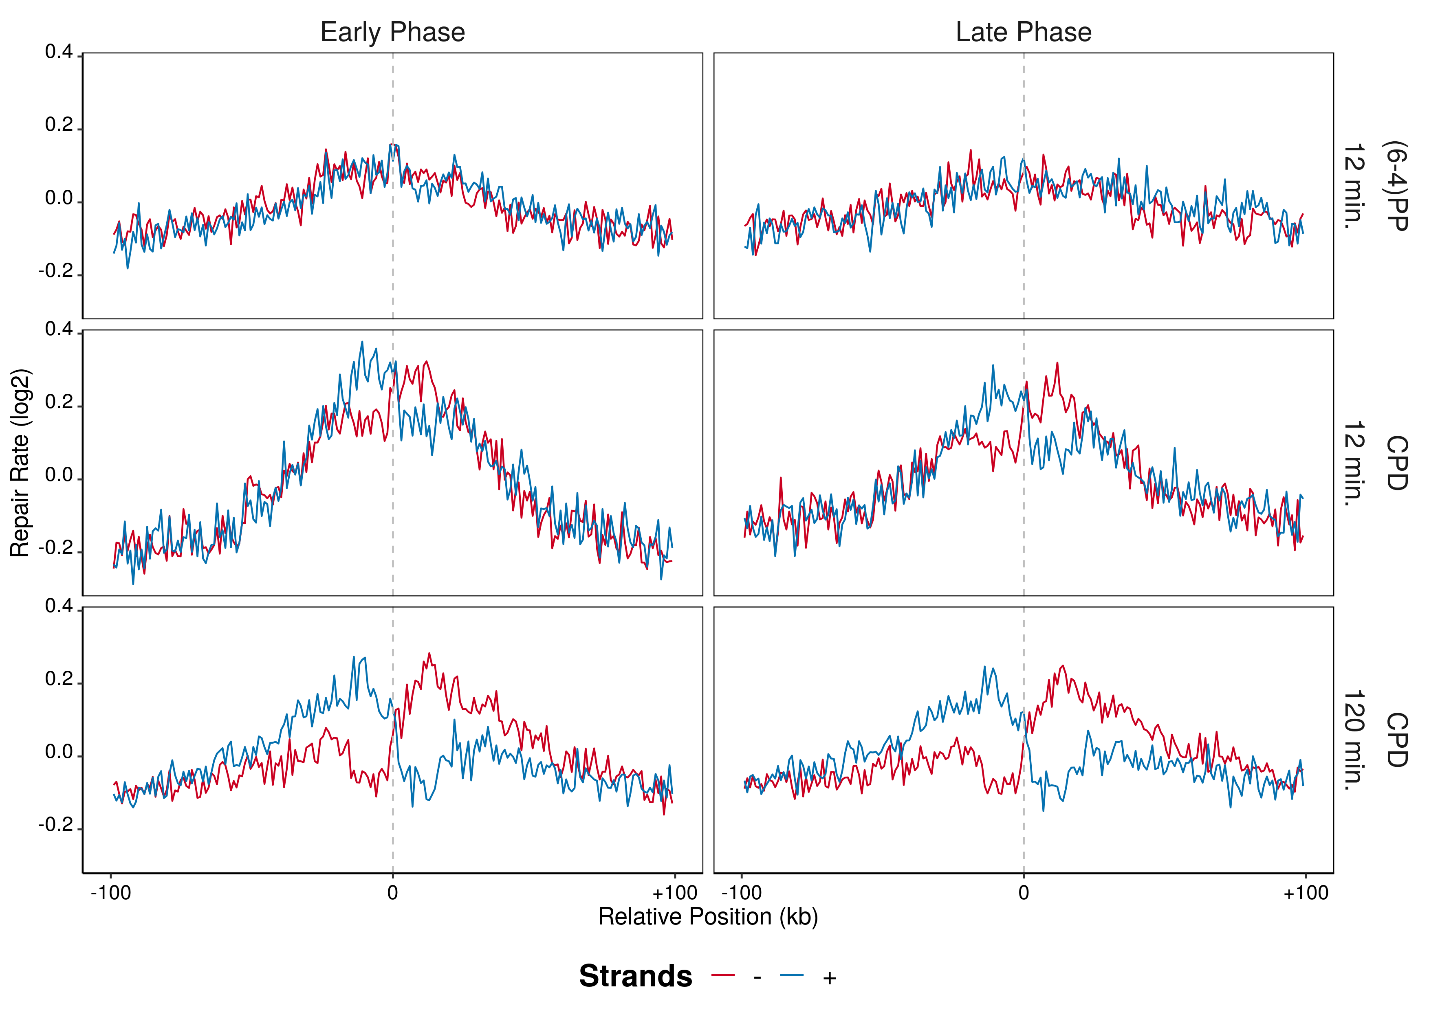
\includegraphics[width=\textwidth]{Chapters/7_appendix/figures/supfig36}
\caption[Repair rate of initiation zones in 200 kb (replicate A).]{Repair rates (XR-seq/Damage-seq) are calculated and log2 transformed in 200 kb windows with 1 kb intervals, which initiation zones are positioned at the center of the region. The blue lines are the plus strands and red lines are the minus strands. Analysis is performed on replicate A.}
\label{supfig:rr200inzonesA}
\end{center}
\end{figure}

\begin{figure}[H]
\begin{center}
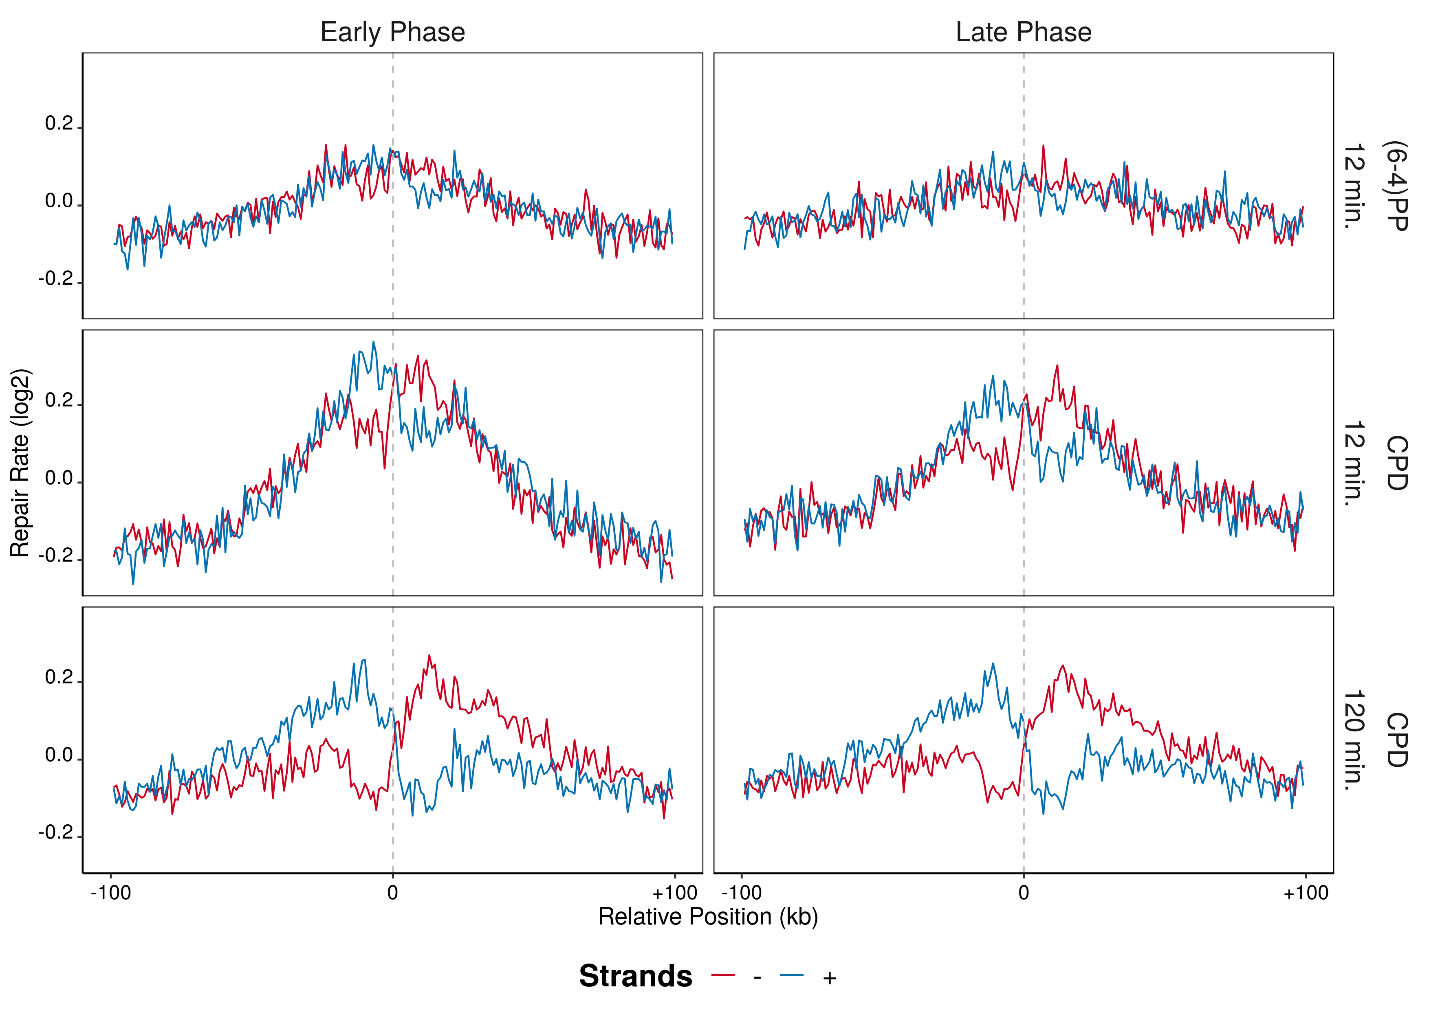
\includegraphics[width=\textwidth]{Chapters/7_appendix/figures/supfig37}
\caption[Repair rate of initiation zones in 200 kb (replicate B).]{Repair rates (XR-seq/Damage-seq) are calculated and log2 transformed in 200 kb windows with 1 kb intervals, which initiation zones are positioned at the center of the region. The blue lines are the plus strands and red lines are the minus strands. Analysis is performed on replicate B.}
\label{supfig:rr200inzonesB}
\end{center}
\end{figure}

\begin{figure}[H]
\begin{center}
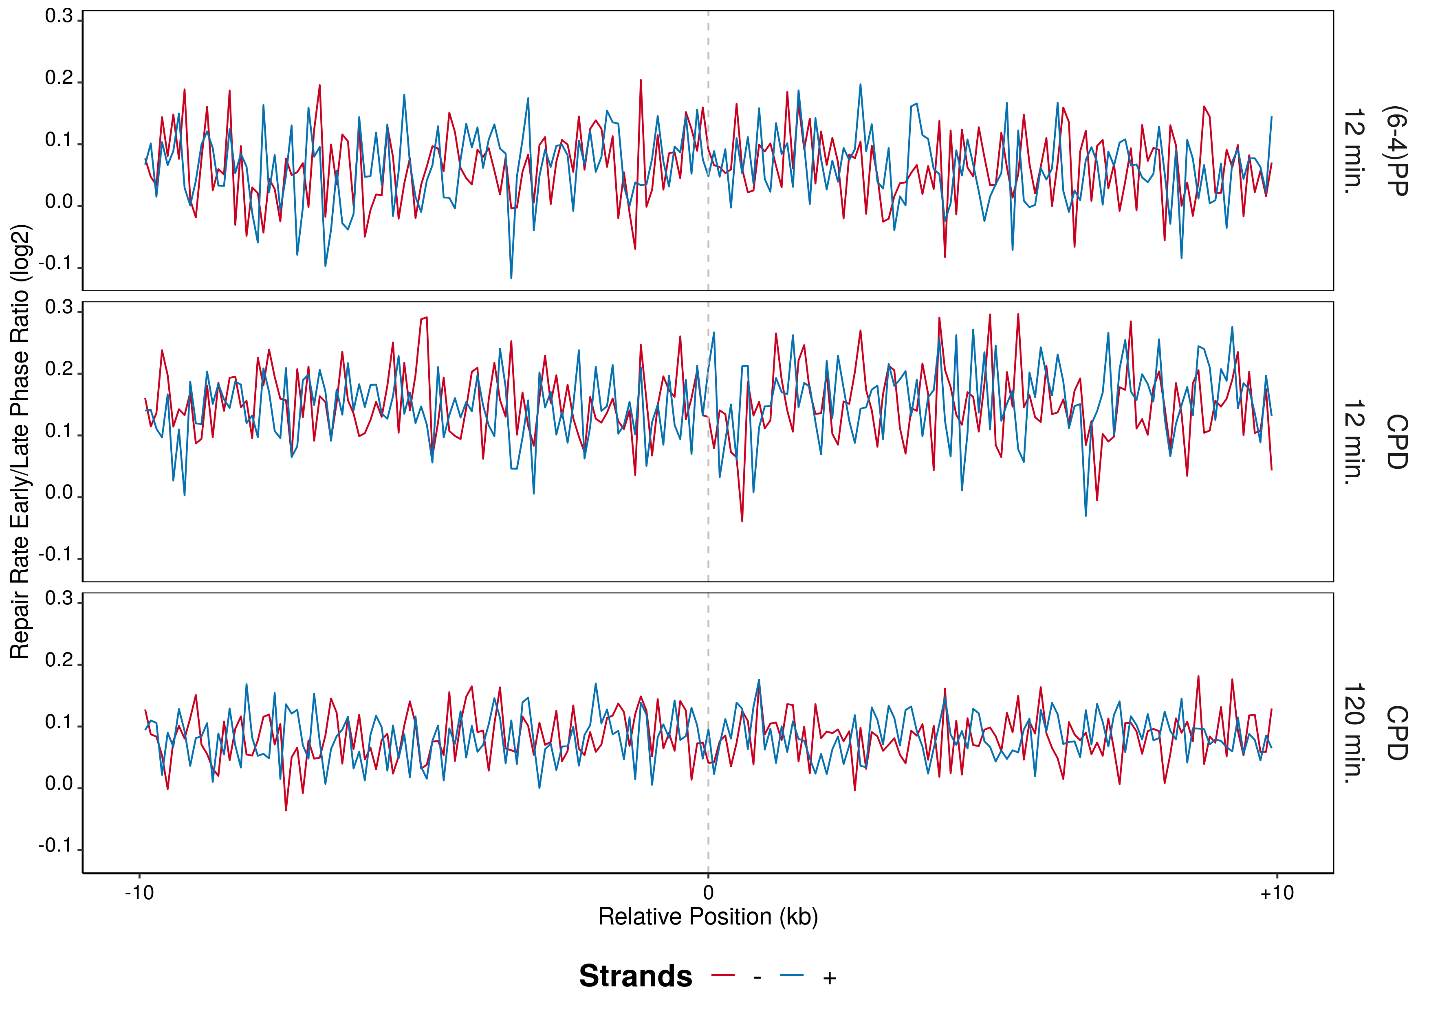
\includegraphics[width=\textwidth]{Chapters/7_appendix/figures/supfig38}
\caption[Repair rate early/late ratio of initiation zones in 20 kb (replicate A).]{After log2 transformed repair rates (XR-seq/Damage-seq) are calculated, samples that are at early S phase of the cell cycle are further divided by the ones that are at the late S phase (early/late) in 20 kb windows with 100 base pair intervals, which initiation zones are positioned at the center of the region. The blue lines are the plus strands and red lines are the minus strands. Analysis is performed on replicate A.}
\label{supfig:rrel20inzonesA}
\end{center}
\end{figure}

\begin{figure}[H]
\begin{center}
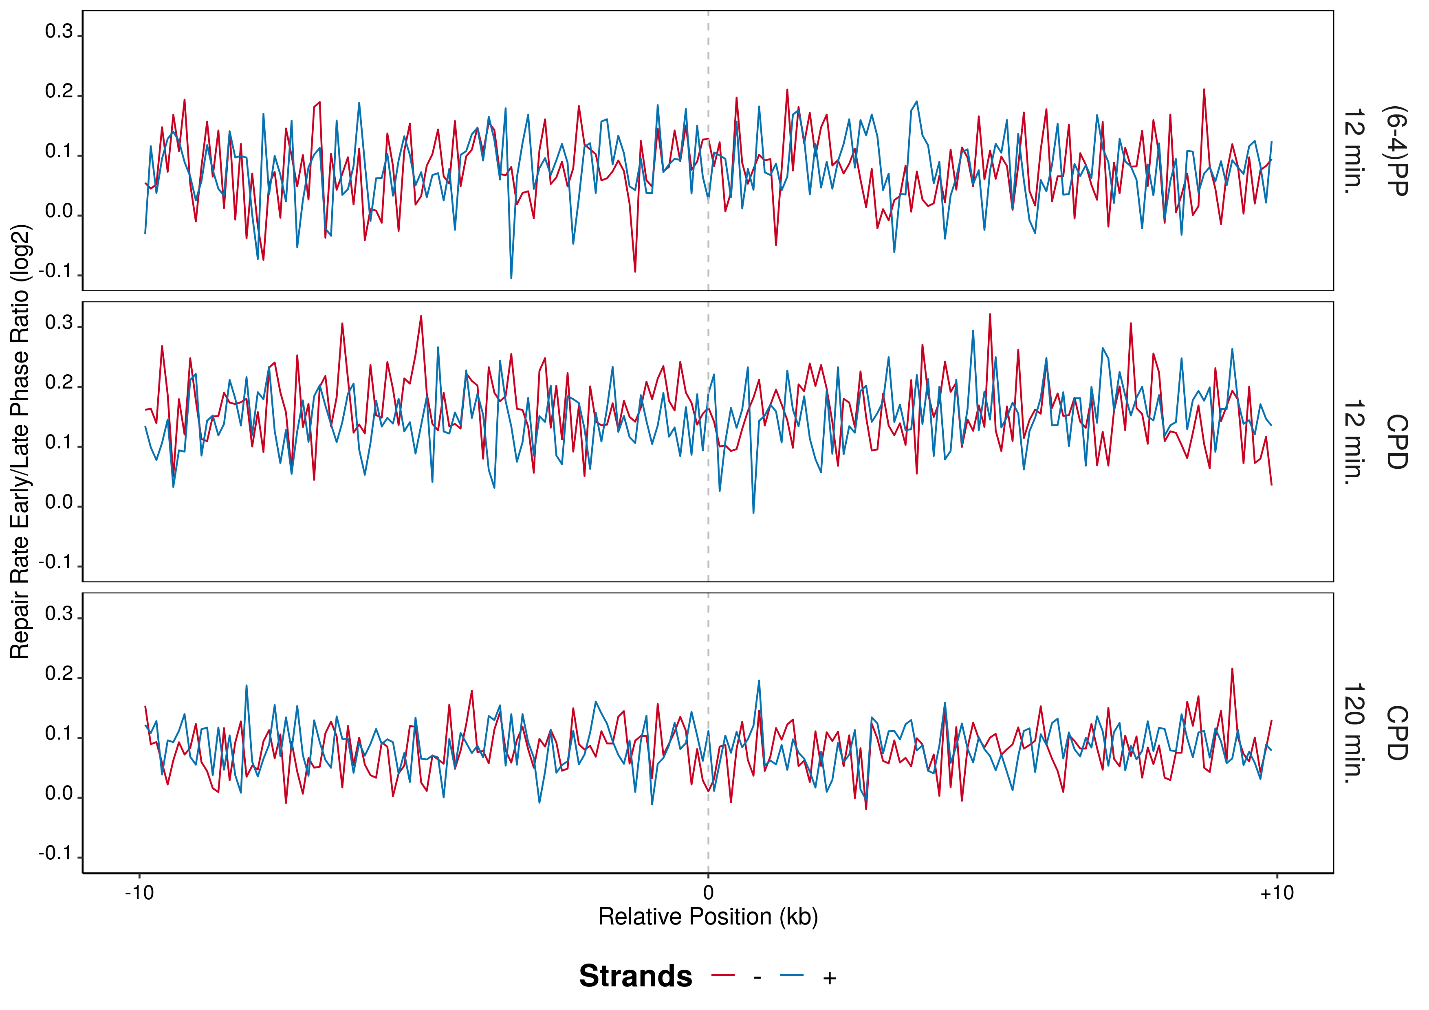
\includegraphics[width=\textwidth]{Chapters/7_appendix/figures/supfig39}
\caption[Repair rate early/late ratio of initiation zones in 20 kb (replicate B).]{After log2 transformed repair rates (XR-seq/Damage-seq) are calculated, samples that are at early S phase of the cell cycle are further divided by the ones that are at the late S phase (early/late) in 20 kb windows with 100 base pair intervals, which initiation zones are positioned at the center of the region. The blue lines are the plus strands and red lines are the minus strands. Analysis is performed on replicate B.}
\label{supfig:rrel20inzonesB}
\end{center}
\end{figure}

\begin{figure}[H]
\begin{center}
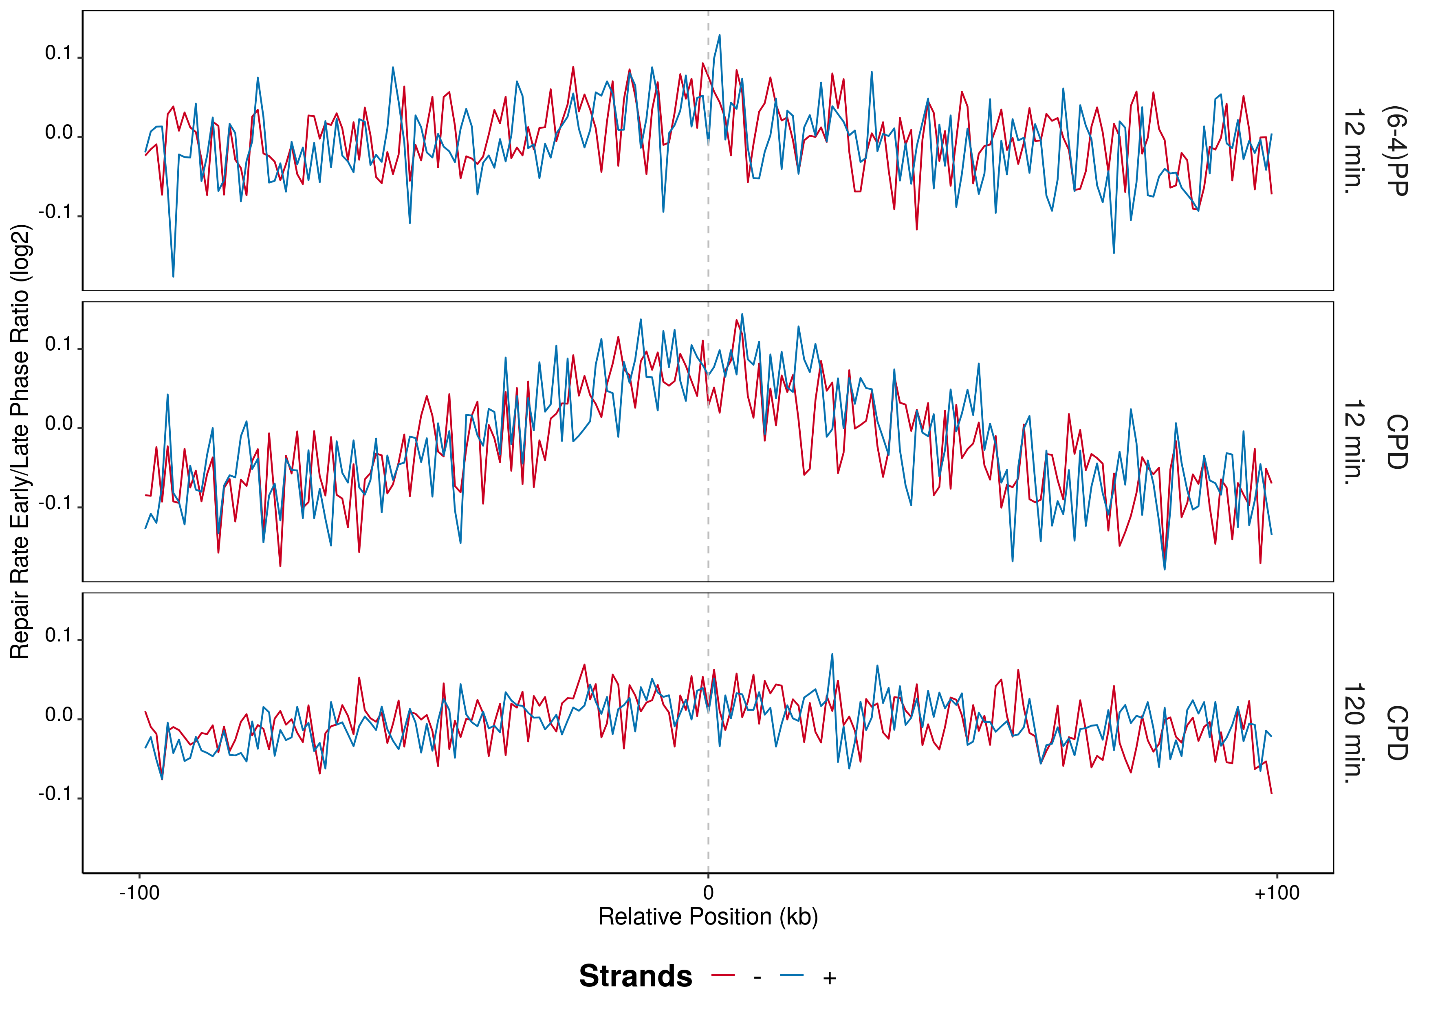
\includegraphics[width=\textwidth]{Chapters/7_appendix/figures/supfig40}
\caption[Repair rate early/late ratio of initiation zones in 200 kb (replicate A).]{After log2 transformed repair rates (XR-seq/Damage-seq) are calculated, samples that are at early S phase of the cell cycle are further divided by the ones that are at the late S phase (early/late) in 200 kb windows with 1 kb intervals, which initiation zones are positioned at the center of the region. The blue lines are the plus strands and red lines are the minus strands. Analysis is performed on replicate A.}
\label{supfig:rrel200inzonesA}
\end{center}
\end{figure}

\begin{figure}[H]
\begin{center}
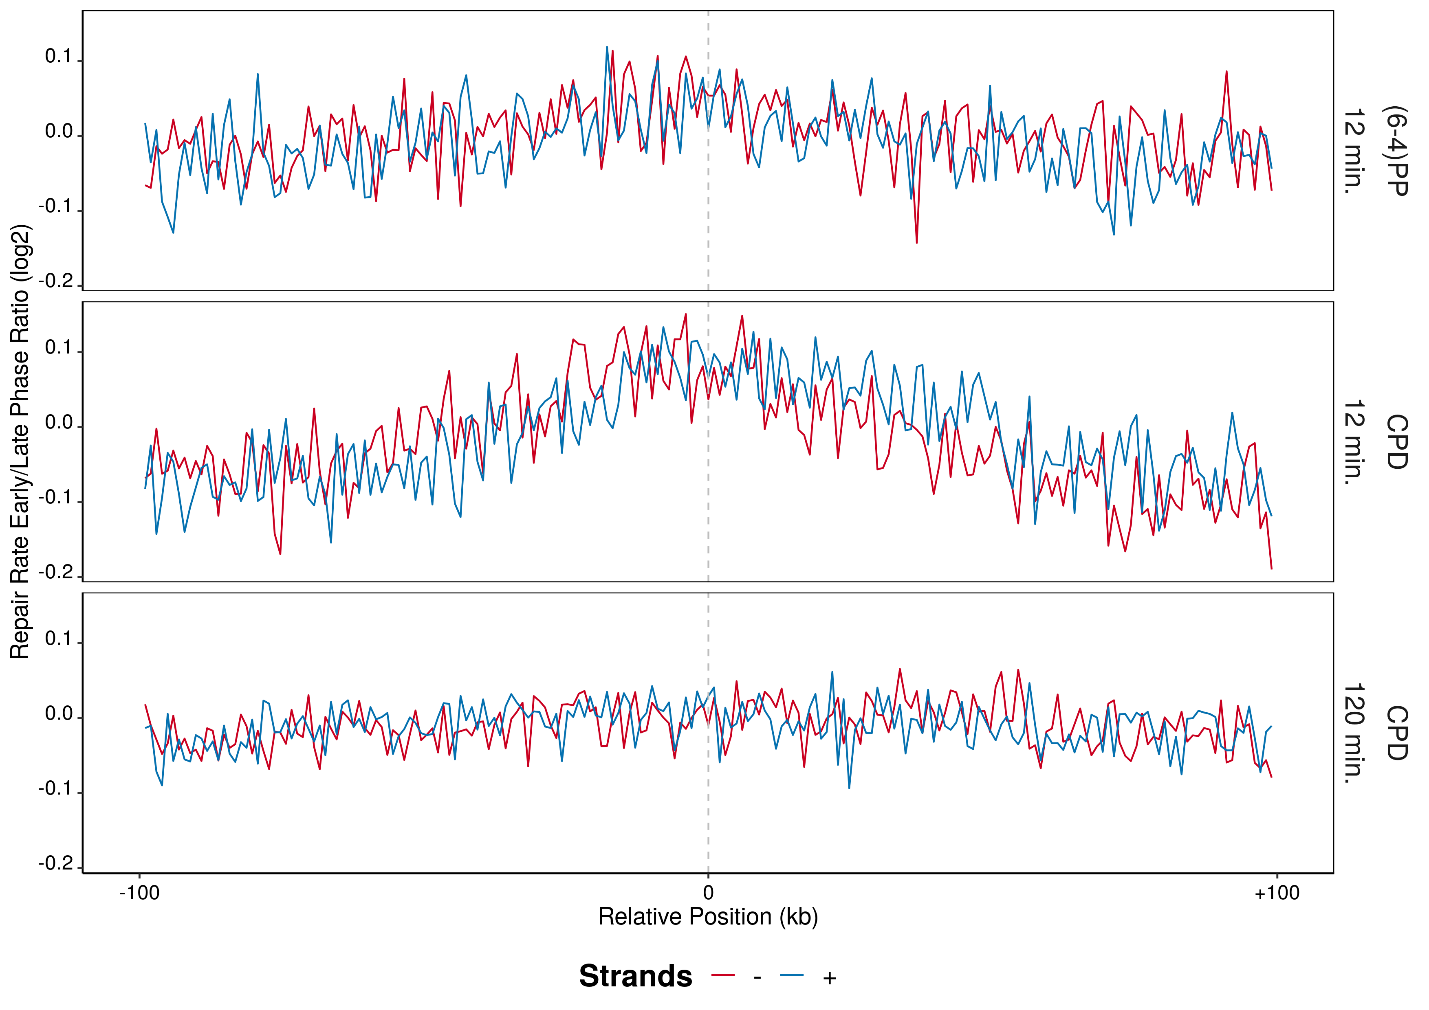
\includegraphics[width=\textwidth]{Chapters/7_appendix/figures/supfig41}
\caption[Repair rate early/late ratio of initiation zones in 200 kb (replicate B).]{After log2 transformed repair rates (XR-seq/Damage-seq) are calculated, samples that are at early S phase of the cell cycle are further divided by the ones that are at the late S phase (early/late) in 200 kb windows with 1 kb intervals, which initiation zones are positioned at the center of the region. The blue lines are the plus strands and red lines are the minus strands. Analysis is performed on replicate B.}
\label{supfig:rrel200inzonesB}
\end{center}
\end{figure}

\begin{figure}[H]
\begin{center}
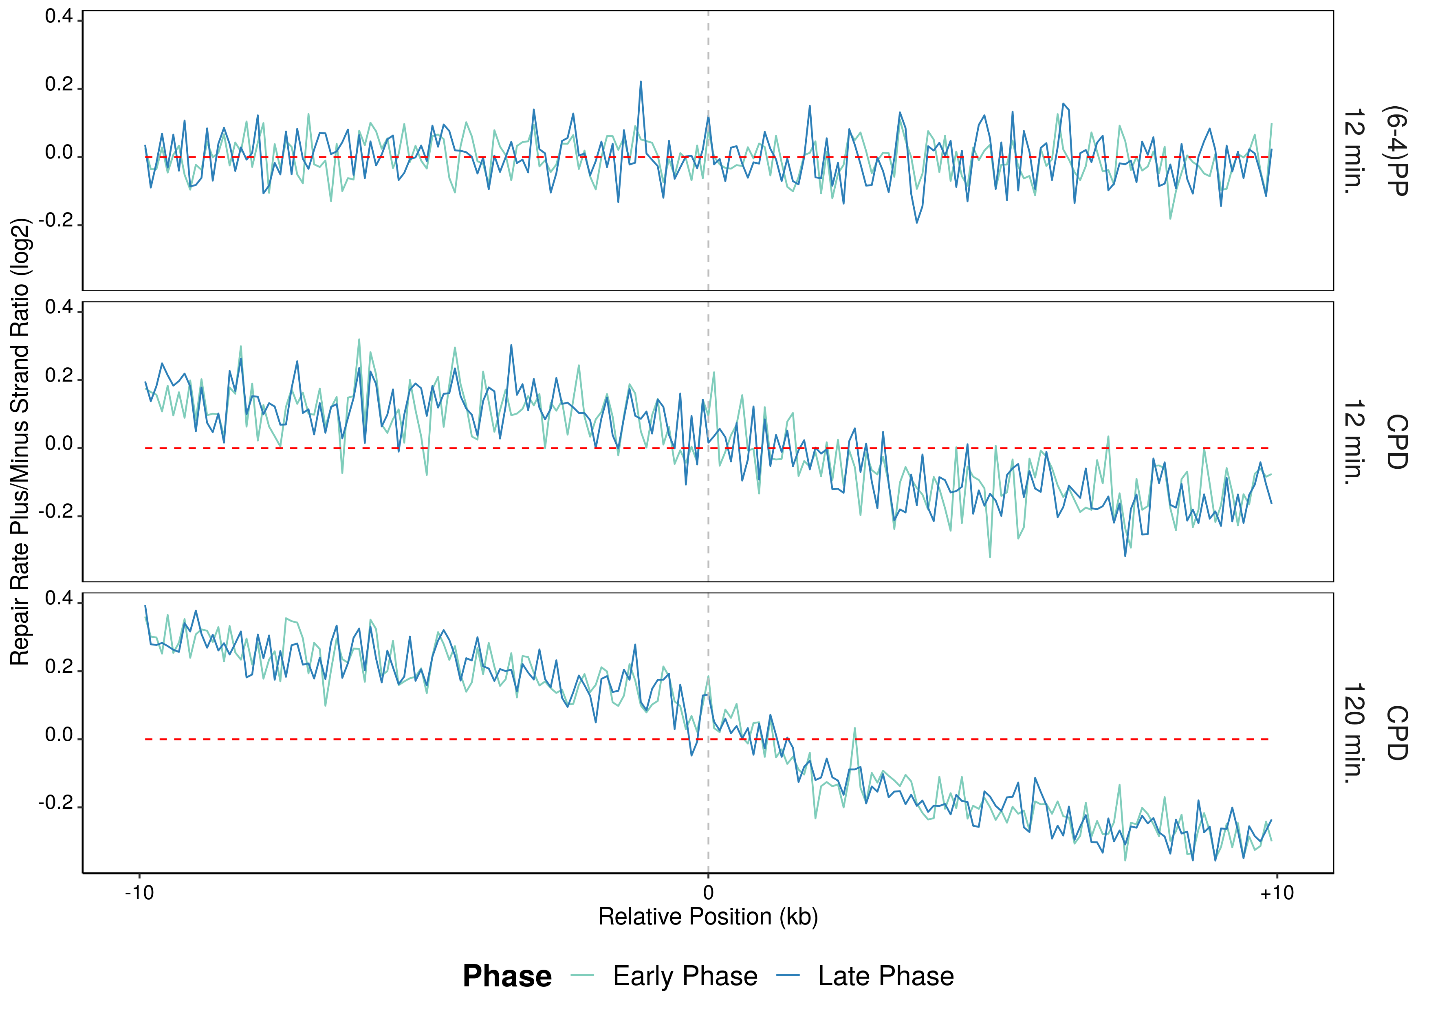
\includegraphics[width=\textwidth]{Chapters/7_appendix/figures/supfig42}
\caption[]{}
\label{supfig:}
\end{center}
\end{figure}

\begin{figure}[H]
\begin{center}
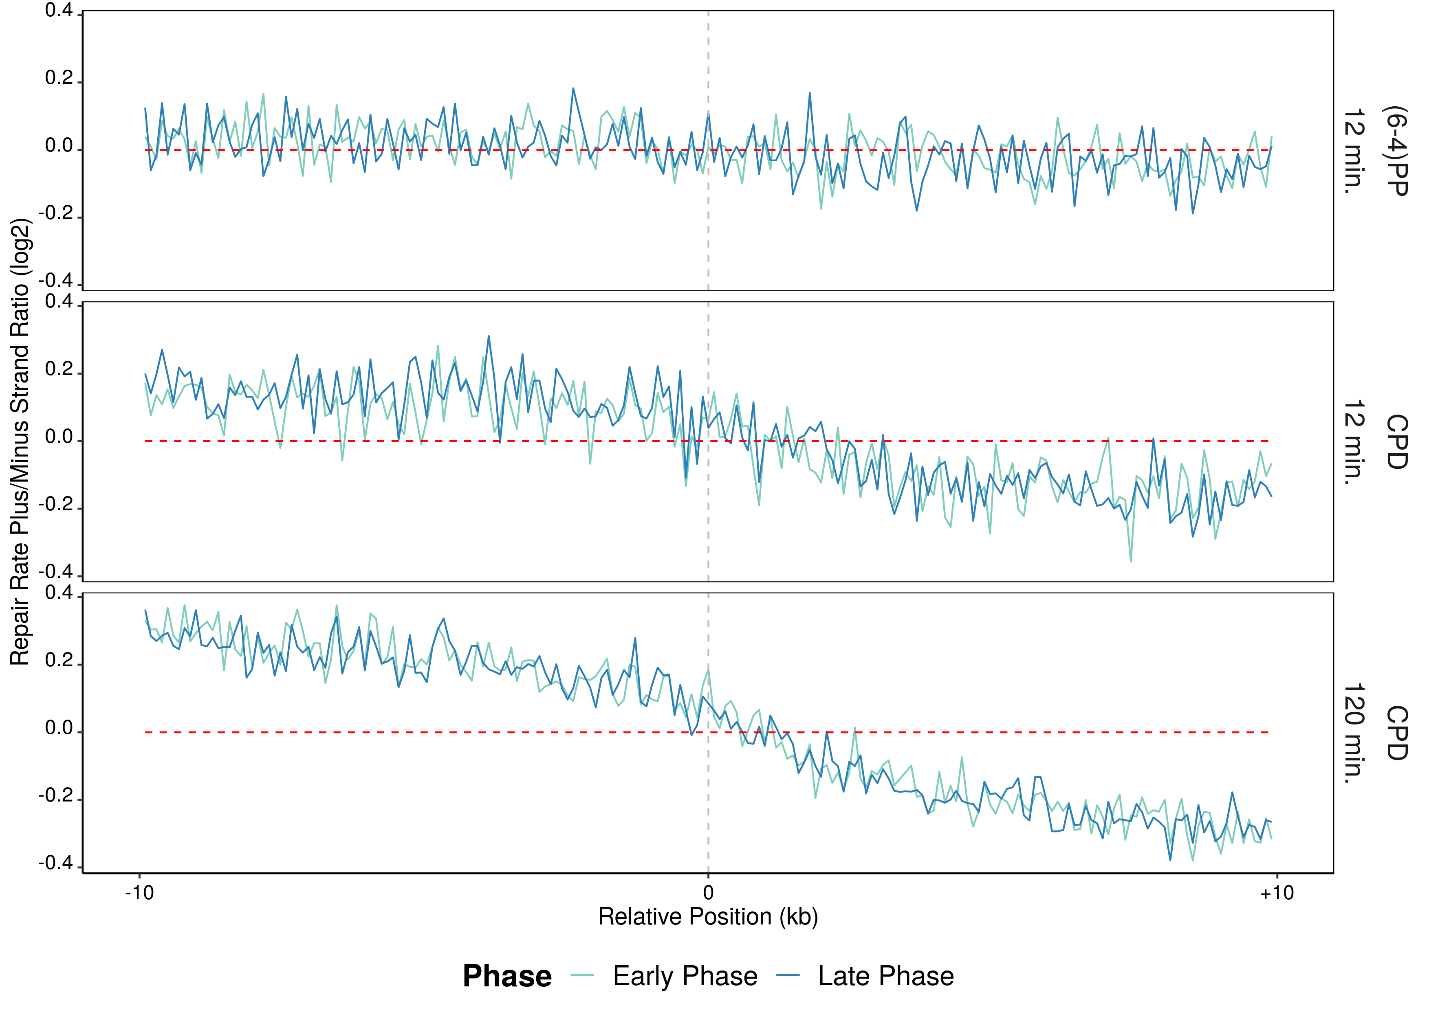
\includegraphics[width=\textwidth]{Chapters/7_appendix/figures/supfig43}
\caption[]{}
\label{supfig:}
\end{center}
\end{figure}

\begin{figure}[H]
\begin{center}
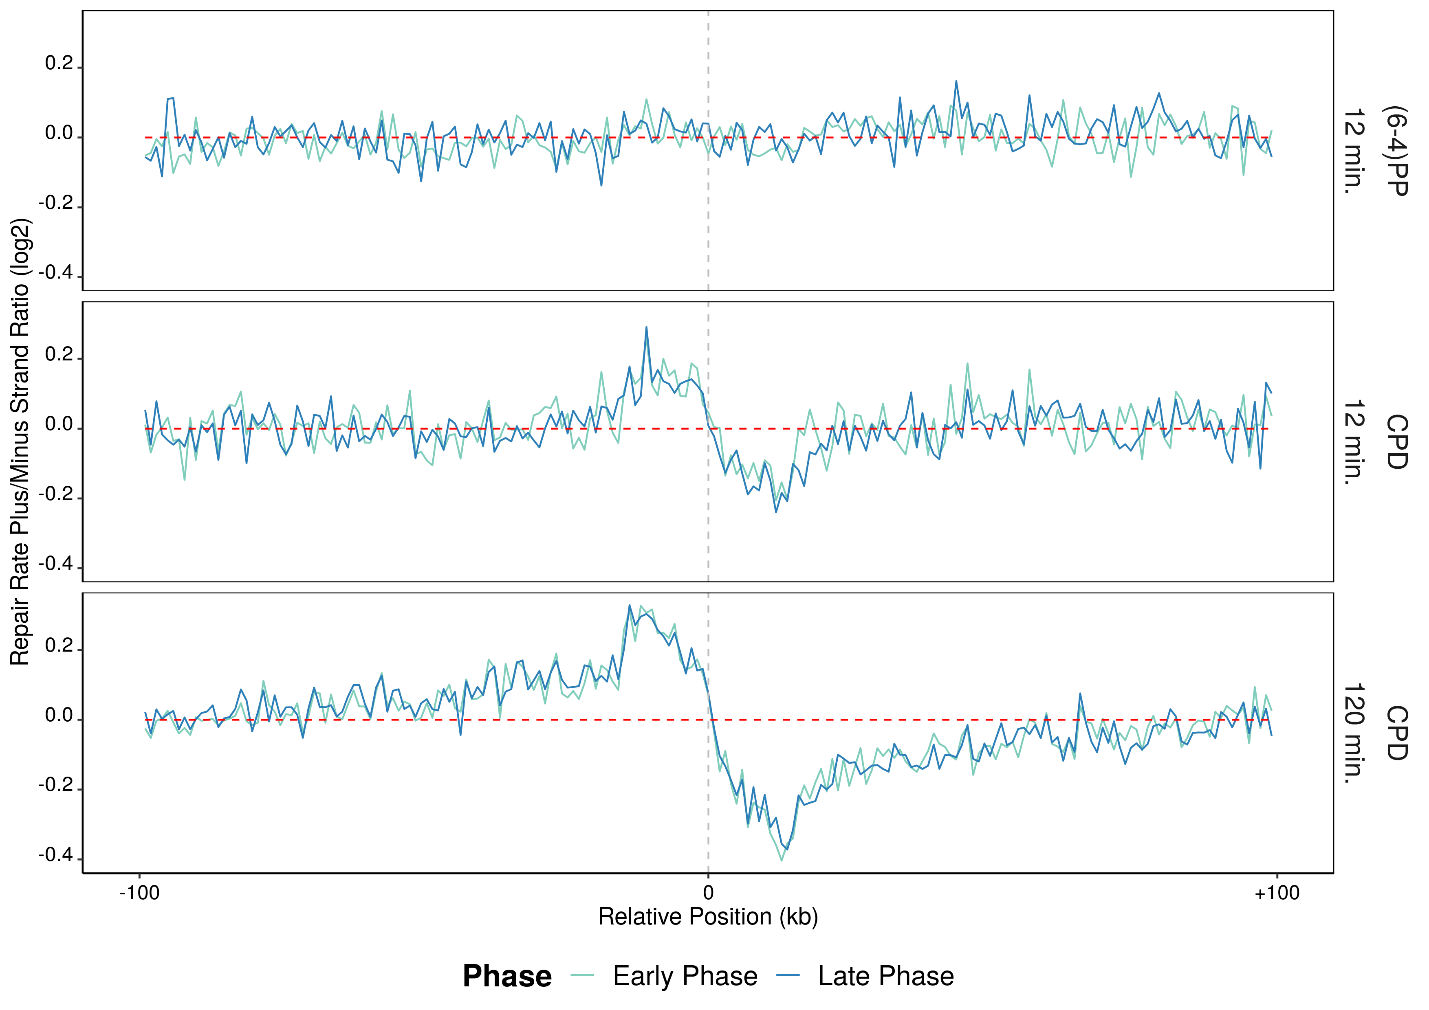
\includegraphics[width=\textwidth]{Chapters/7_appendix/figures/supfig44}
\caption[]{}
\label{supfig:}
\end{center}
\end{figure}

\begin{figure}[H]
\begin{center}
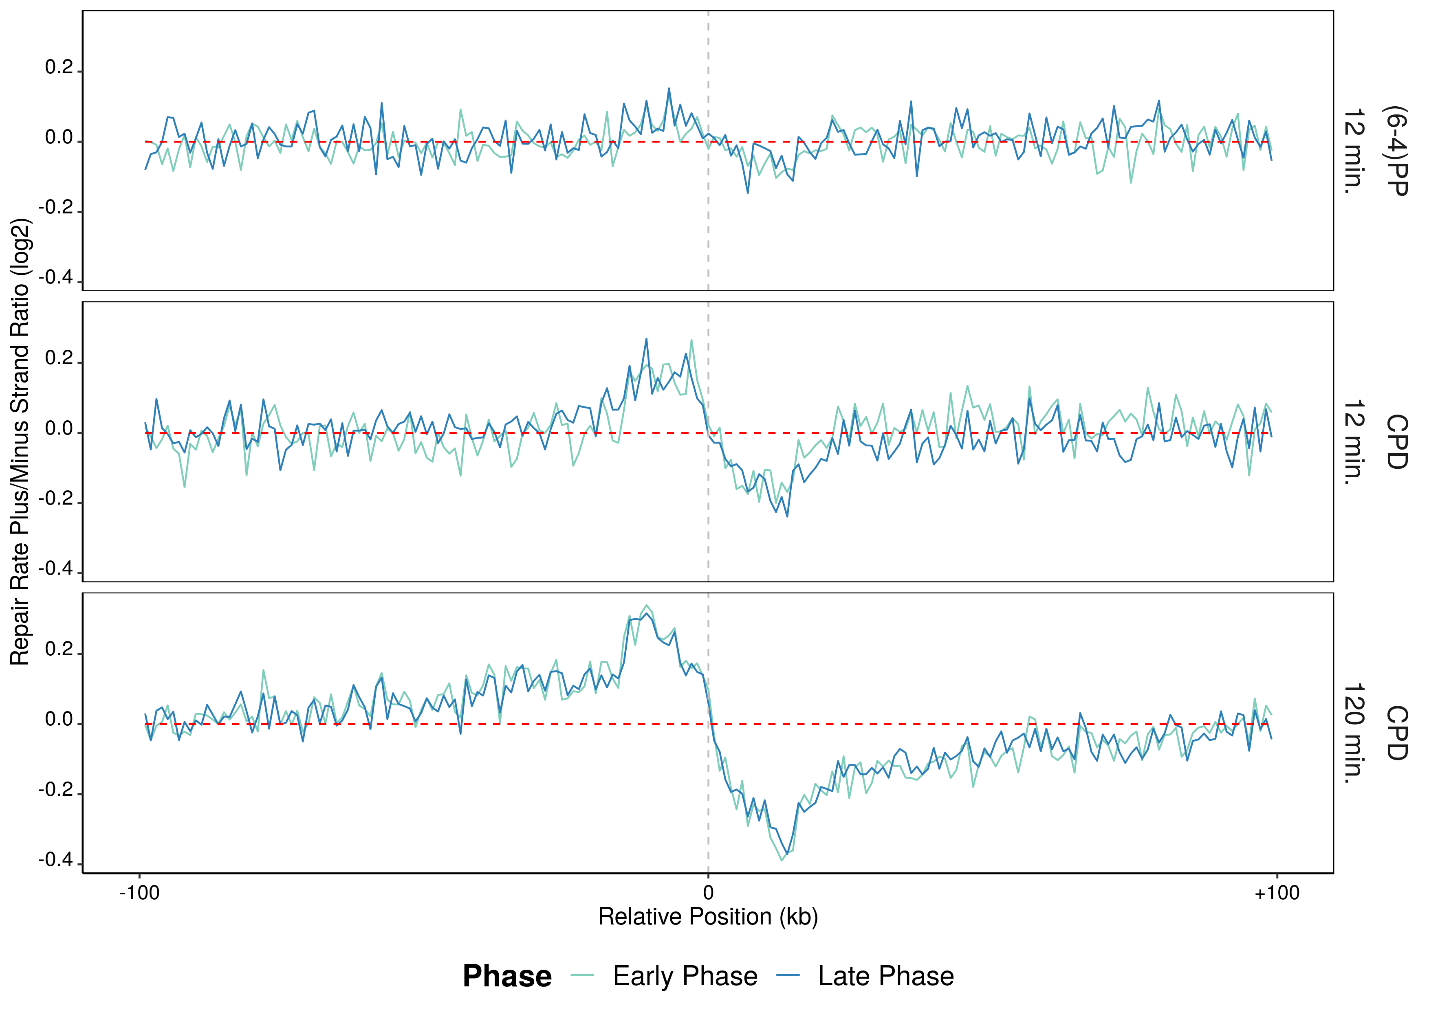
\includegraphics[width=\textwidth]{Chapters/7_appendix/figures/supfig45}
\caption[]{}
\label{supfig:}
\end{center}
\end{figure}

\begin{figure}[H]
\begin{center}
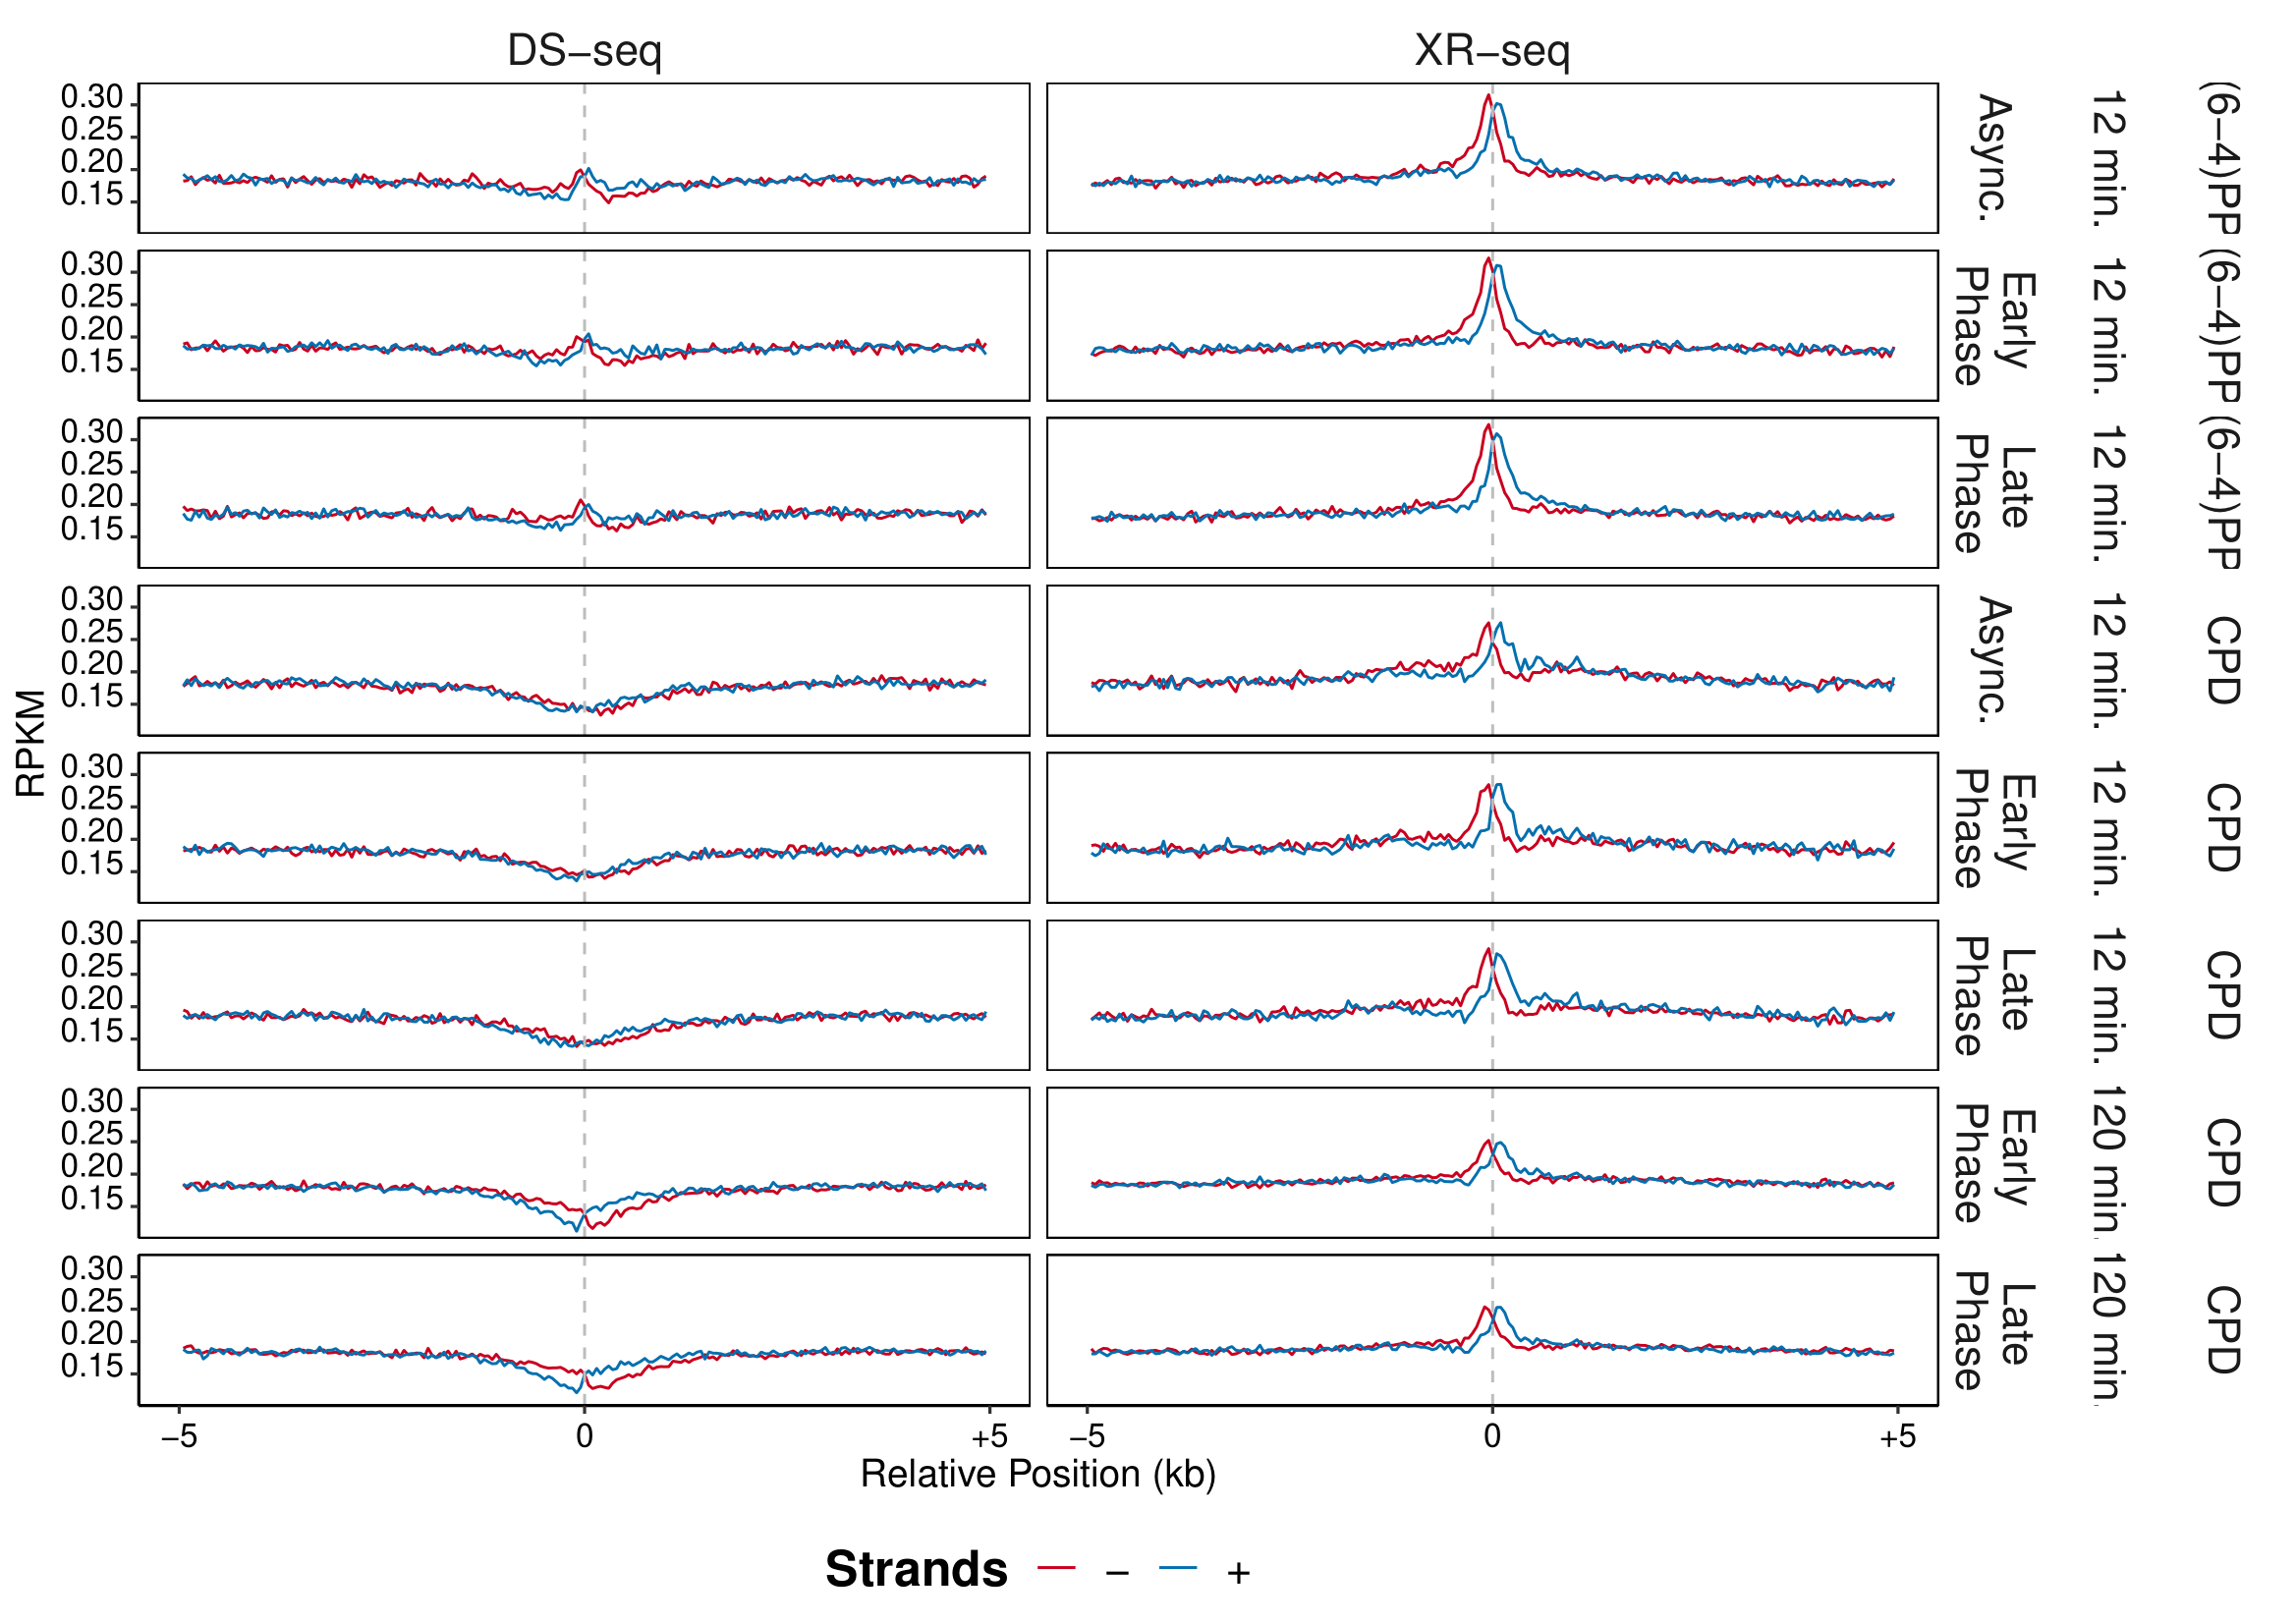
\includegraphics[width=\textwidth]{Chapters/7_appendix/figures/supfig46}
\caption[]{}
\label{supfig:}
\end{center}
\end{figure}

\begin{figure}[H]
\begin{center}
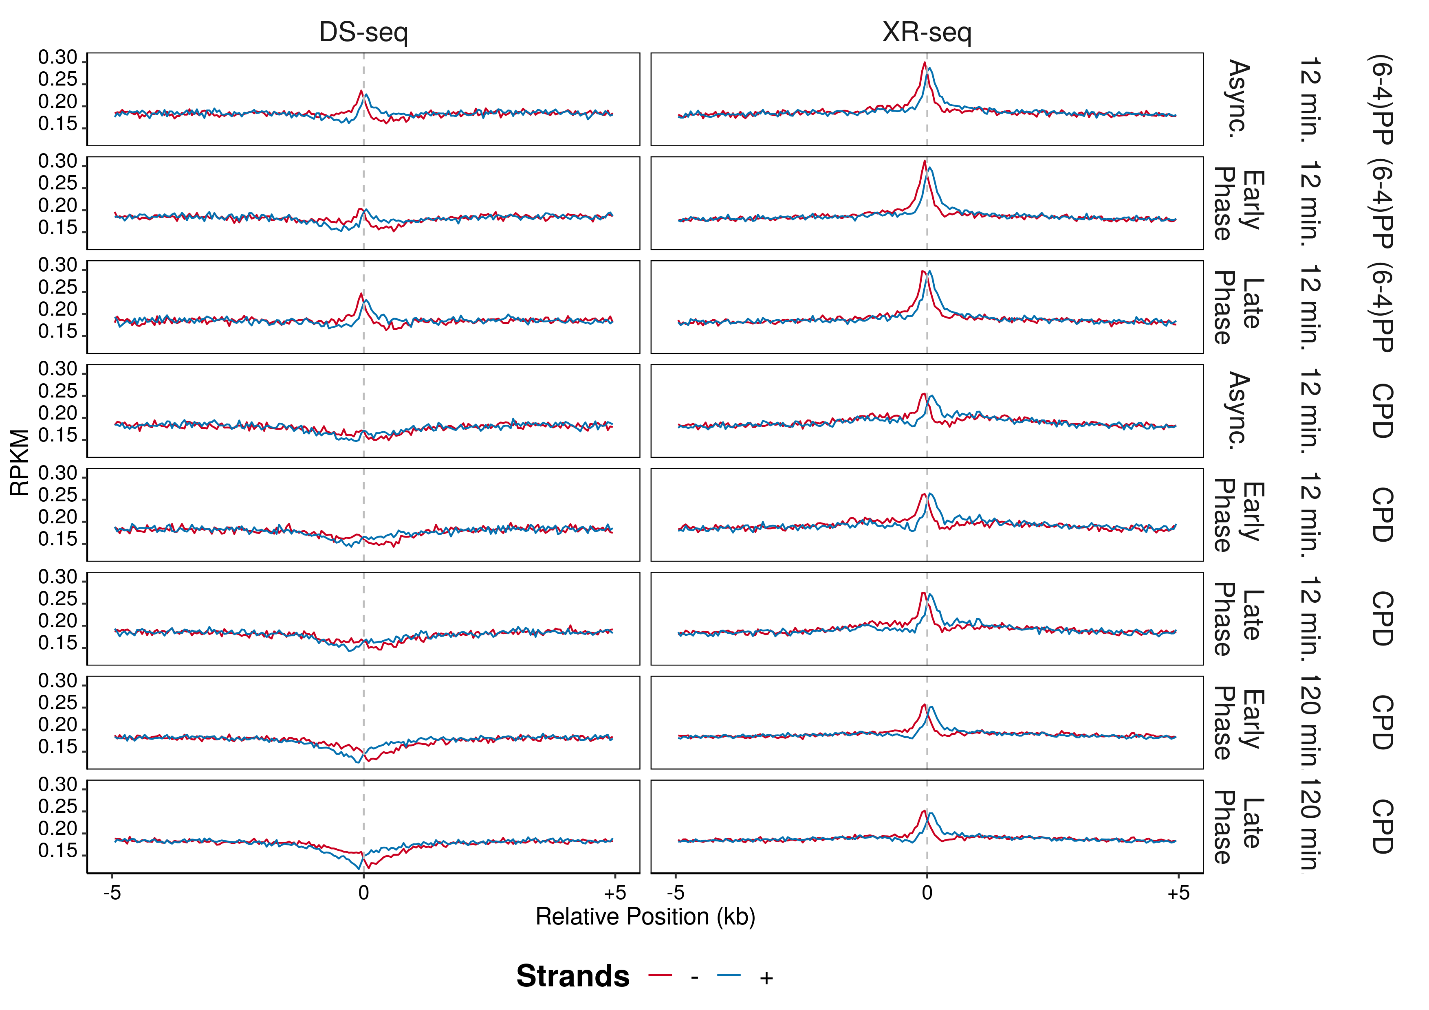
\includegraphics[width=\textwidth]{Chapters/7_appendix/figures/supfig47}
\caption[]{}
\label{supfig:}
\end{center}
\end{figure}

\begin{figure}[H]
\begin{center}
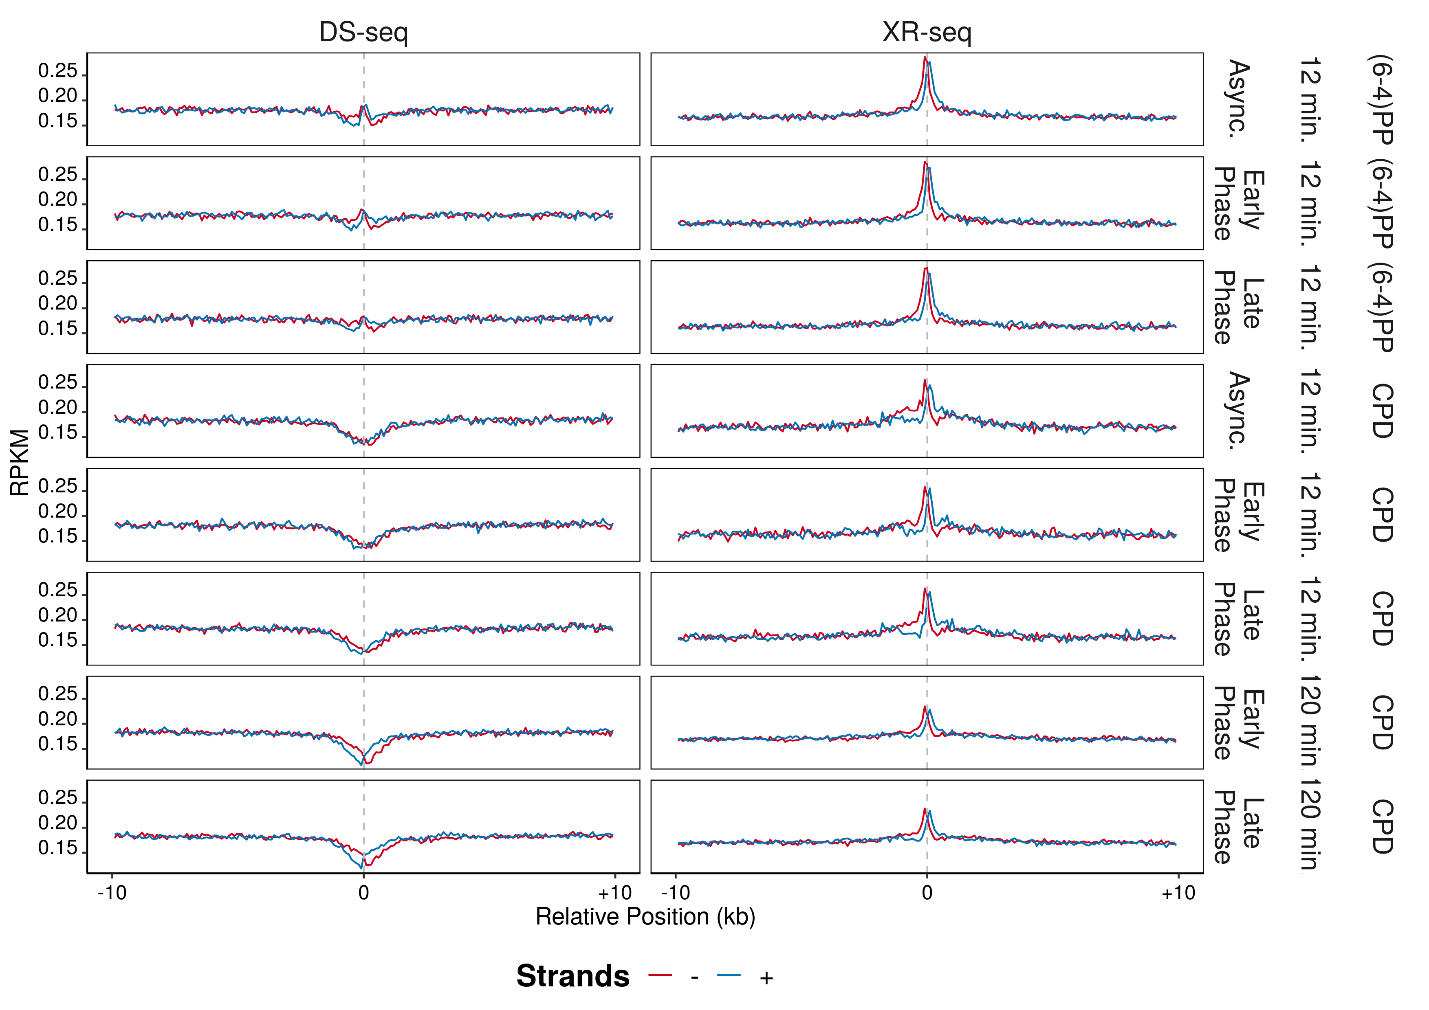
\includegraphics[width=\textwidth]{Chapters/7_appendix/figures/supfig48}
\caption[]{}
\label{supfig:}
\end{center}
\end{figure}

\begin{figure}[H]
\begin{center}
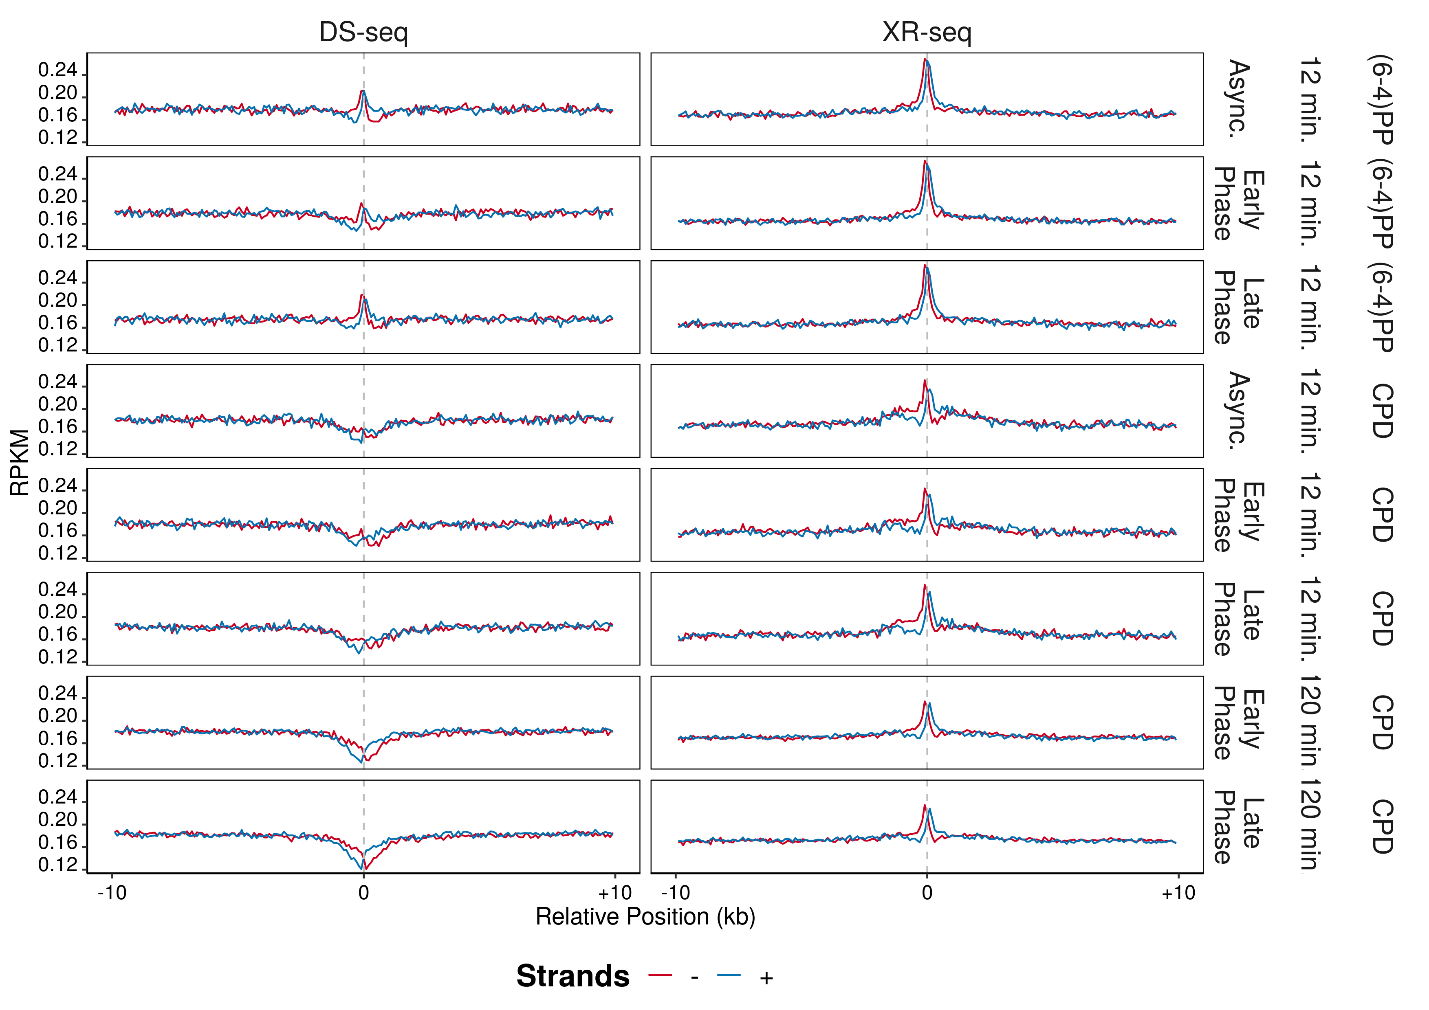
\includegraphics[width=\textwidth]{Chapters/7_appendix/figures/supfig49}
\caption[]{}
\label{supfig:}
\end{center}
\end{figure}

\begin{figure}[H]
\begin{center}
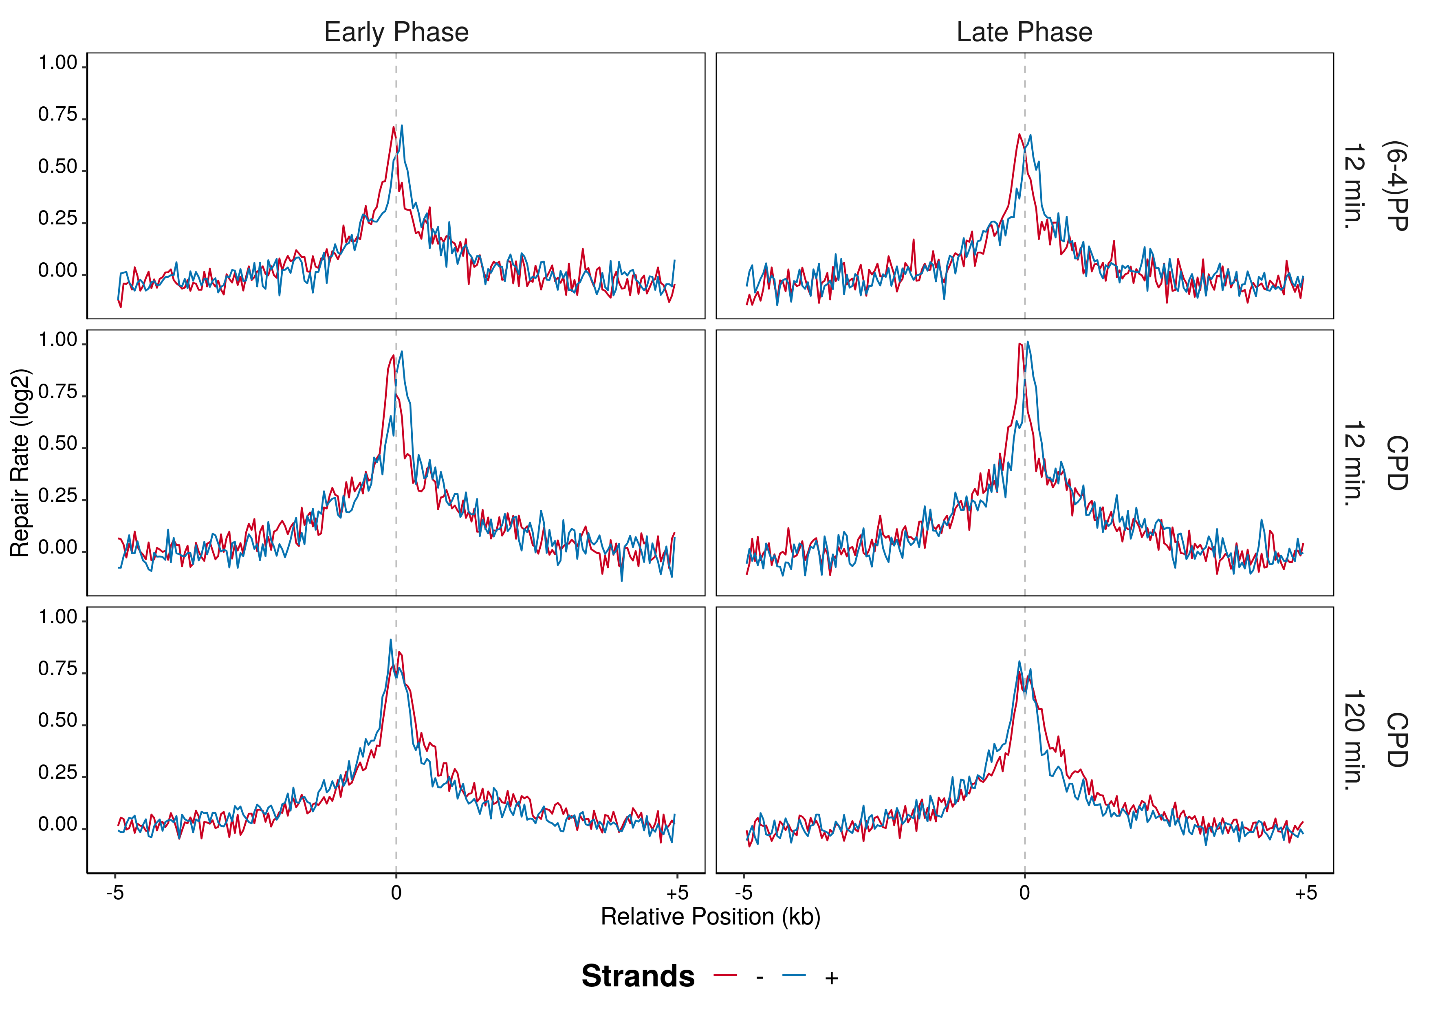
\includegraphics[width=\textwidth]{Chapters/7_appendix/figures/supfig50}
\caption[]{}
\label{supfig:}
\end{center}
\end{figure}

\begin{figure}[H]
\begin{center}
\includegraphics[width=\textwidth]{Chapters/7_appendix/figures/supfig51}
\caption[]{}
\label{supfig:}
\end{center}
\end{figure}

\begin{figure}[H]
\begin{center}
\includegraphics[width=\textwidth]{Chapters/7_appendix/figures/supfig52}
\caption[]{}
\label{supfig:}
\end{center}
\end{figure}

\begin{figure}[H]
\begin{center}
\includegraphics[width=\textwidth]{Chapters/7_appendix/figures/supfig53}
\caption[]{}
\label{supfig:}
\end{center}
\end{figure}

\begin{figure}[H]
\begin{center}
\includegraphics[width=\textwidth]{Chapters/7_appendix/figures/supfig54}
\caption[]{}
\label{supfig:}
\end{center}
\end{figure}

\begin{figure}[H]
\begin{center}
\includegraphics[width=\textwidth]{Chapters/7_appendix/figures/supfig55}
\caption[]{}
\label{supfig:}
\end{center}
\end{figure}

\begin{figure}[H]
\begin{center}
\includegraphics[width=\textwidth]{Chapters/7_appendix/figures/supfig56}
\caption[]{}
\label{supfig:}
\end{center}
\end{figure}

\begin{figure}[H]
\begin{center}
\includegraphics[width=\textwidth]{Chapters/7_appendix/figures/supfig57}
\caption[]{}
\label{supfig:}
\end{center}
\end{figure}

\begin{figure}[H]
\begin{center}
\includegraphics[width=\textwidth]{Chapters/7_appendix/figures/supfig58}
\caption[]{}
\label{supfig:}
\end{center}
\end{figure}

\begin{figure}[H]
\begin{center}
\includegraphics[width=\textwidth]{Chapters/7_appendix/figures/supfig59}
\caption[]{}
\label{supfig:}
\end{center}
\end{figure}

\begin{figure}[H]
\begin{center}
\includegraphics[width=\textwidth]{Chapters/7_appendix/figures/supfig60}
\caption[]{}
\label{supfig:}
\end{center}
\end{figure}

\begin{figure}[H]
\begin{center}
\includegraphics[width=\textwidth]{Chapters/7_appendix/figures/supfig61}
\caption[]{}
\label{supfig:}
\end{center}
\end{figure}

\begin{figure}[H]
\begin{center}
\includegraphics[width=\textwidth]{Chapters/7_appendix/figures/supfig62}
\caption[]{}
\label{supfig:}
\end{center}
\end{figure}

\begin{figure}[H]
\begin{center}
\includegraphics[width=\textwidth]{Chapters/7_appendix/figures/supfig63}
\caption[]{}
\label{supfig:}
\end{center}
\end{figure}

\begin{figure}[H]
\begin{center}
\includegraphics[width=\textwidth]{Chapters/7_appendix/figures/supfig64}
\caption[]{}
\label{supfig:}
\end{center}
\end{figure}

\begin{figure}[H]
\begin{center}
\includegraphics[width=\textwidth]{Chapters/7_appendix/figures/supfig65}
\caption[]{}
\label{supfig:}
\end{center}
\end{figure}

\begin{figure}[H]
\begin{center}
\includegraphics[width=\textwidth]{Chapters/7_appendix/figures/supfig66}
\caption[]{}
\label{supfig:}
\end{center}
\end{figure}

\begin{figure}[H]
\begin{center}
\includegraphics[width=\textwidth]{Chapters/7_appendix/figures/supfig67}
\caption[]{}
\label{supfig:}
\end{center}
\end{figure}

\begin{figure}[H]
\begin{center}
\includegraphics[width=\textwidth]{Chapters/7_appendix/figures/supfig68}
\caption[]{}
\label{supfig:}
\end{center}
\end{figure}

\begin{figure}[H]
\begin{center}
\includegraphics[width=\textwidth]{Chapters/7_appendix/figures/supfig69}
\caption[]{}
\label{supfig:}
\end{center}
\end{figure}

\begin{figure}[H]
\begin{center}
\includegraphics[width=\textwidth]{Chapters/7_appendix/figures/supfig70}
\caption[]{}
\label{supfig:}
\end{center}
\end{figure}

\begin{figure}[H]
\begin{center}
\includegraphics[width=\textwidth]{Chapters/7_appendix/figures/supfig71}
\caption[]{}
\label{supfig:}
\end{center}
\end{figure}

\begin{figure}[H]
\begin{center}
\includegraphics[width=\textwidth]{Chapters/7_appendix/figures/supfig72}
\caption[]{}
\label{supfig:}
\end{center}
\end{figure}

\begin{figure}[H]
\begin{center}
\includegraphics[width=\textwidth]{Chapters/7_appendix/figures/supfig73}
\caption[]{}
\label{supfig:}
\end{center}
\end{figure}

\begin{figure}[H]
\begin{center}
\includegraphics[width=\textwidth]{Chapters/7_appendix/figures/supfig74}
\caption[]{}
\label{supfig:}
\end{center}
\end{figure}

\begin{figure}[H]
\begin{center}
\includegraphics[width=\textwidth]{Chapters/7_appendix/figures/supfig75}
\caption[]{}
\label{supfig:}
\end{center}
\end{figure}

\begin{figure}[H]
\begin{center}
\includegraphics[width=\textwidth]{Chapters/7_appendix/figures/supfig76}
\caption[]{}
\label{supfig:}
\end{center}
\end{figure}

\begin{figure}[H]
\begin{center}
\includegraphics[width=\textwidth]{Chapters/7_appendix/figures/supfig77}
\caption[]{}
\label{supfig:}
\end{center}
\end{figure}

\begin{figure}[H]
\begin{center}
\includegraphics[width=\textwidth]{Chapters/7_appendix/figures/supfig78}
\caption[]{}
\label{supfig:}
\end{center}
\end{figure}

\begin{figure}[H]
\begin{center}
\includegraphics[width=\textwidth]{Chapters/7_appendix/figures/supfig79}
\caption[]{}
\label{supfig:}
\end{center}
\end{figure}
